\documentclass[twoside]{book}

% Packages required by doxygen
\usepackage{fixltx2e}
\usepackage{calc}
\usepackage{doxygen}
\usepackage[export]{adjustbox} % also loads graphicx
\usepackage{graphicx}
\usepackage[utf8]{inputenc}
\usepackage{makeidx}
\usepackage{multicol}
\usepackage{multirow}
\PassOptionsToPackage{warn}{textcomp}
\usepackage{textcomp}
\usepackage[nointegrals]{wasysym}
\usepackage[table]{xcolor}

% Font selection
\usepackage[T1]{fontenc}
\usepackage[scaled=.90]{helvet}
\usepackage{courier}
\usepackage{amssymb}
\usepackage{sectsty}
\renewcommand{\familydefault}{\sfdefault}
\allsectionsfont{%
  \fontseries{bc}\selectfont%
  \color{darkgray}%
}
\renewcommand{\DoxyLabelFont}{%
  \fontseries{bc}\selectfont%
  \color{darkgray}%
}
\newcommand{\+}{\discretionary{\mbox{\scriptsize$\hookleftarrow$}}{}{}}

% Page & text layout
\usepackage{geometry}
\geometry{%
  a4paper,%
  top=2.5cm,%
  bottom=2.5cm,%
  left=2.5cm,%
  right=2.5cm%
}
\tolerance=750
\hfuzz=15pt
\hbadness=750
\setlength{\emergencystretch}{15pt}
\setlength{\parindent}{0cm}
\setlength{\parskip}{3ex plus 2ex minus 2ex}
\makeatletter
\renewcommand{\paragraph}{%
  \@startsection{paragraph}{4}{0ex}{-1.0ex}{1.0ex}{%
    \normalfont\normalsize\bfseries\SS@parafont%
  }%
}
\renewcommand{\subparagraph}{%
  \@startsection{subparagraph}{5}{0ex}{-1.0ex}{1.0ex}{%
    \normalfont\normalsize\bfseries\SS@subparafont%
  }%
}
\makeatother

% Headers & footers
\usepackage{fancyhdr}
\pagestyle{fancyplain}
\fancyhead[LE]{\fancyplain{}{\bfseries\thepage}}
\fancyhead[CE]{\fancyplain{}{}}
\fancyhead[RE]{\fancyplain{}{\bfseries\leftmark}}
\fancyhead[LO]{\fancyplain{}{\bfseries\rightmark}}
\fancyhead[CO]{\fancyplain{}{}}
\fancyhead[RO]{\fancyplain{}{\bfseries\thepage}}
\fancyfoot[LE]{\fancyplain{}{}}
\fancyfoot[CE]{\fancyplain{}{}}
\fancyfoot[RE]{\fancyplain{}{\bfseries\scriptsize Generated by Doxygen }}
\fancyfoot[LO]{\fancyplain{}{\bfseries\scriptsize Generated by Doxygen }}
\fancyfoot[CO]{\fancyplain{}{}}
\fancyfoot[RO]{\fancyplain{}{}}
\renewcommand{\footrulewidth}{0.4pt}
\renewcommand{\chaptermark}[1]{%
  \markboth{#1}{}%
}
\renewcommand{\sectionmark}[1]{%
  \markright{\thesection\ #1}%
}

% Indices & bibliography
\usepackage{natbib}
\usepackage[titles]{tocloft}
\setcounter{tocdepth}{3}
\setcounter{secnumdepth}{5}
\makeindex

% Hyperlinks (required, but should be loaded last)
\usepackage{ifpdf}
\ifpdf
  \usepackage[pdftex,pagebackref=true]{hyperref}
\else
  \usepackage[ps2pdf,pagebackref=true]{hyperref}
\fi
\hypersetup{%
  colorlinks=true,%
  linkcolor=blue,%
  citecolor=blue,%
  unicode%
}

% Custom commands
\newcommand{\clearemptydoublepage}{%
  \newpage{\pagestyle{empty}\cleardoublepage}%
}

\usepackage{caption}
\captionsetup{labelsep=space,justification=centering,font={bf},singlelinecheck=off,skip=4pt,position=top}

%===== C O N T E N T S =====

\begin{document}

% Titlepage & ToC
\hypersetup{pageanchor=false,
             bookmarksnumbered=true,
             pdfencoding=unicode
            }
\pagenumbering{roman}
\begin{titlepage}
\vspace*{7cm}
\begin{center}%
{\Large My Project }\\
\vspace*{1cm}
{\large Generated by Doxygen 1.8.11}\\
\end{center}
\end{titlepage}
\clearemptydoublepage
\tableofcontents
\clearemptydoublepage
\pagenumbering{arabic}
\hypersetup{pageanchor=true}

%--- Begin generated contents ---
\chapter{Namespace Index}
\section{Packages}
Here are the packages with brief descriptions (if available)\+:\begin{DoxyCompactList}
\item\contentsline{section}{\hyperlink{namespace_editor_u_i}{Editor\+UI} }{\pageref{namespace_editor_u_i}}{}
\item\contentsline{section}{\hyperlink{namespace_v_m_e}{V\+ME} }{\pageref{namespace_v_m_e}}{}
\item\contentsline{section}{\hyperlink{namespace_v_m_e_1_1_settings}{V\+M\+E.\+Settings} }{\pageref{namespace_v_m_e_1_1_settings}}{}
\item\contentsline{section}{\hyperlink{namespace_v_s_e}{V\+SE} }{\pageref{namespace_v_s_e}}{}
\end{DoxyCompactList}

\chapter{Hierarchical Index}
\section{Class Hierarchy}
This inheritance list is sorted roughly, but not completely, alphabetically\+:\begin{DoxyCompactList}
\item \contentsline{section}{Asset\+Creation}{\pageref{class_asset_creation}}{}
\item \contentsline{section}{Base\+Editor\+Group}{\pageref{class_base_editor_group}}{}
\begin{DoxyCompactList}
\item \contentsline{section}{V\+S\+E\+Header}{\pageref{class_v_s_e_header}}{}
\end{DoxyCompactList}
\item \contentsline{section}{Base\+Editor\+Panel}{\pageref{class_base_editor_panel}}{}
\begin{DoxyCompactList}
\item \contentsline{section}{Editor\+Search\+Window}{\pageref{class_editor_search_window}}{}
\item \contentsline{section}{V\+M\+E.\+Editor\+Panel\+Template}{\pageref{class_v_m_e_1_1_editor_panel_template}}{}
\item \contentsline{section}{V\+M\+E.\+Settings.\+V\+M\+E\+Settings\+Key\+Panel}{\pageref{class_v_m_e_1_1_settings_1_1_v_m_e_settings_key_panel}}{}
\item \contentsline{section}{V\+M\+E.\+V\+M\+E\+Chunk\+Panel}{\pageref{class_v_m_e_1_1_v_m_e_chunk_panel}}{}
\item \contentsline{section}{V\+M\+E.\+V\+M\+E\+File\+Manager\+Panel}{\pageref{class_v_m_e_1_1_v_m_e_file_manager_panel}}{}
\item \contentsline{section}{V\+M\+E.\+V\+M\+E\+Main\+Panel}{\pageref{class_v_m_e_1_1_v_m_e_main_panel}}{}
\item \contentsline{section}{V\+M\+E.\+V\+M\+E\+Mode\+Panel}{\pageref{class_v_m_e_1_1_v_m_e_mode_panel}}{}
\item \contentsline{section}{V\+M\+E.\+V\+M\+E\+Voxel\+Swatch\+Panel}{\pageref{class_v_m_e_1_1_v_m_e_voxel_swatch_panel}}{}
\end{DoxyCompactList}
\item \contentsline{section}{Editor\+U\+I.\+Draw}{\pageref{class_editor_u_i_1_1_draw}}{}
\item Editor\+Window\begin{DoxyCompactList}
\item \contentsline{section}{V\+M\+E.\+Settings.\+V\+M\+E\+Settings\+Window}{\pageref{class_v_m_e_1_1_settings_1_1_v_m_e_settings_window}}{}
\item \contentsline{section}{V\+M\+E.\+V\+M\+E\+Main\+Window}{\pageref{class_v_m_e_1_1_v_m_e_main_window}}{}
\item \contentsline{section}{V\+S\+E.\+V\+S\+E\+Window}{\pageref{class_v_s_e_1_1_v_s_e_window}}{}
\end{DoxyCompactList}
\item Mono\+Behaviour\begin{DoxyCompactList}
\item \contentsline{section}{Chunk}{\pageref{class_chunk}}{}
\item \contentsline{section}{Chunk\+Object\+Data}{\pageref{class_chunk_object_data}}{}
\item \contentsline{section}{Chunk\+Spawner}{\pageref{class_chunk_spawner}}{}
\item \contentsline{section}{V\+M\+E\+Menu\+Item}{\pageref{class_v_m_e_menu_item}}{}
\item \contentsline{section}{V\+M\+E\+Picker\+Controls}{\pageref{class_v_m_e_picker_controls}}{}
\item \contentsline{section}{Voxel\+Map}{\pageref{class_voxel_map}}{}
\end{DoxyCompactList}
\item \contentsline{section}{Quick\+Reference}{\pageref{class_quick_reference}}{}
\item Scriptable\+Object\begin{DoxyCompactList}
\item \contentsline{section}{V\+M\+E\+Settings\+Object}{\pageref{class_v_m_e_settings_object}}{}
\item \contentsline{section}{Voxel\+Swatch}{\pageref{class_voxel_swatch}}{}
\end{DoxyCompactList}
\item \contentsline{section}{V\+M\+E.\+V\+M\+E\+Edit\+Controls}{\pageref{class_v_m_e_1_1_v_m_e_edit_controls}}{}
\item \contentsline{section}{V\+M\+E.\+V\+M\+E\+Global}{\pageref{class_v_m_e_1_1_v_m_e_global}}{}
\item \contentsline{section}{V\+M\+E.\+V\+M\+E\+Paint\+Controls}{\pageref{class_v_m_e_1_1_v_m_e_paint_controls}}{}
\item \contentsline{section}{V\+M\+E.\+V\+M\+E\+Selection\+Controls}{\pageref{class_v_m_e_1_1_v_m_e_selection_controls}}{}
\item \contentsline{section}{V\+M\+E.\+V\+M\+E\+Selection\+Panel}{\pageref{class_v_m_e_1_1_v_m_e_selection_panel}}{}
\item \contentsline{section}{V\+M\+E.\+V\+M\+E\+Snap\+Panel}{\pageref{class_v_m_e_1_1_v_m_e_snap_panel}}{}
\item \contentsline{section}{V\+M\+E\+Tile\+Add\+Controls}{\pageref{class_v_m_e_tile_add_controls}}{}
\item \contentsline{section}{V\+S\+Category}{\pageref{class_v_s_category}}{}
\item \contentsline{section}{V\+S\+Item\+Group}{\pageref{class_v_s_item_group}}{}
\end{DoxyCompactList}

\chapter{Class Index}
\section{Class List}
Here are the classes, structs, unions and interfaces with brief descriptions\+:\begin{DoxyCompactList}
\item\contentsline{section}{\hyperlink{class_asset_creation}{Asset\+Creation} }{\pageref{class_asset_creation}}{}
\item\contentsline{section}{\hyperlink{class_base_editor_group}{Base\+Editor\+Group} \\*Base\+Class for a Editor Group. same as Panel but without a toggle state }{\pageref{class_base_editor_group}}{}
\item\contentsline{section}{\hyperlink{class_base_editor_panel}{Base\+Editor\+Panel} \\*Base\+Class for a Editor Panel }{\pageref{class_base_editor_panel}}{}
\item\contentsline{section}{\hyperlink{class_chunk}{Chunk} }{\pageref{class_chunk}}{}
\item\contentsline{section}{\hyperlink{class_chunk_object_data}{Chunk\+Object\+Data} }{\pageref{class_chunk_object_data}}{}
\item\contentsline{section}{\hyperlink{class_chunk_spawner}{Chunk\+Spawner} \\*Spawn chunk inside the editor, and save it. }{\pageref{class_chunk_spawner}}{}
\item\contentsline{section}{\hyperlink{class_editor_u_i_1_1_draw}{Editor\+U\+I.\+Draw} \\*Fancier UI functions. }{\pageref{class_editor_u_i_1_1_draw}}{}
\item\contentsline{section}{\hyperlink{class_v_m_e_1_1_editor_panel_template}{V\+M\+E.\+Editor\+Panel\+Template} }{\pageref{class_v_m_e_1_1_editor_panel_template}}{}
\item\contentsline{section}{\hyperlink{class_editor_search_window}{Editor\+Search\+Window} }{\pageref{class_editor_search_window}}{}
\item\contentsline{section}{\hyperlink{class_quick_reference}{Quick\+Reference} }{\pageref{class_quick_reference}}{}
\item\contentsline{section}{\hyperlink{class_v_m_e_1_1_v_m_e_chunk_panel}{V\+M\+E.\+V\+M\+E\+Chunk\+Panel} \\*Panel used for the Chunks in the \hyperlink{namespace_v_m_e}{V\+ME} Editor. }{\pageref{class_v_m_e_1_1_v_m_e_chunk_panel}}{}
\item\contentsline{section}{\hyperlink{class_v_m_e_1_1_v_m_e_edit_controls}{V\+M\+E.\+V\+M\+E\+Edit\+Controls} \\*Handles all related actions of editing a tile. actions like\+: }{\pageref{class_v_m_e_1_1_v_m_e_edit_controls}}{}
\item\contentsline{section}{\hyperlink{class_v_m_e_1_1_v_m_e_file_manager_panel}{V\+M\+E.\+V\+M\+E\+File\+Manager\+Panel} }{\pageref{class_v_m_e_1_1_v_m_e_file_manager_panel}}{}
\item\contentsline{section}{\hyperlink{class_v_m_e_1_1_v_m_e_global}{V\+M\+E.\+V\+M\+E\+Global} \\*Global functions used on multiple locations thereby easier to reference as a global function. }{\pageref{class_v_m_e_1_1_v_m_e_global}}{}
\item\contentsline{section}{\hyperlink{class_v_m_e_1_1_v_m_e_main_panel}{V\+M\+E.\+V\+M\+E\+Main\+Panel} \\*Voxel Map Main Panel }{\pageref{class_v_m_e_1_1_v_m_e_main_panel}}{}
\item\contentsline{section}{\hyperlink{class_v_m_e_1_1_v_m_e_main_window}{V\+M\+E.\+V\+M\+E\+Main\+Window} \\*Voxel Map Main Editor window }{\pageref{class_v_m_e_1_1_v_m_e_main_window}}{}
\item\contentsline{section}{\hyperlink{class_v_m_e_menu_item}{V\+M\+E\+Menu\+Item} \\*Used for adding \hyperlink{namespace_v_m_e}{V\+ME} related Menu Items. }{\pageref{class_v_m_e_menu_item}}{}
\item\contentsline{section}{\hyperlink{class_v_m_e_1_1_v_m_e_mode_panel}{V\+M\+E.\+V\+M\+E\+Mode\+Panel} }{\pageref{class_v_m_e_1_1_v_m_e_mode_panel}}{}
\item\contentsline{section}{\hyperlink{class_v_m_e_1_1_v_m_e_paint_controls}{V\+M\+E.\+V\+M\+E\+Paint\+Controls} \\*Controls for painting a tile. }{\pageref{class_v_m_e_1_1_v_m_e_paint_controls}}{}
\item\contentsline{section}{\hyperlink{class_v_m_e_picker_controls}{V\+M\+E\+Picker\+Controls} }{\pageref{class_v_m_e_picker_controls}}{}
\item\contentsline{section}{\hyperlink{class_v_m_e_1_1_v_m_e_selection_controls}{V\+M\+E.\+V\+M\+E\+Selection\+Controls} \\*Handles the controls for selecting tiles. }{\pageref{class_v_m_e_1_1_v_m_e_selection_controls}}{}
\item\contentsline{section}{\hyperlink{class_v_m_e_1_1_v_m_e_selection_panel}{V\+M\+E.\+V\+M\+E\+Selection\+Panel} \\*Shows info of current selection }{\pageref{class_v_m_e_1_1_v_m_e_selection_panel}}{}
\item\contentsline{section}{\hyperlink{class_v_m_e_1_1_settings_1_1_v_m_e_settings_key_panel}{V\+M\+E.\+Settings.\+V\+M\+E\+Settings\+Key\+Panel} }{\pageref{class_v_m_e_1_1_settings_1_1_v_m_e_settings_key_panel}}{}
\item\contentsline{section}{\hyperlink{class_v_m_e_settings_object}{V\+M\+E\+Settings\+Object} \\*Holds all personal settings for the editor in a object inside the editor project. }{\pageref{class_v_m_e_settings_object}}{}
\item\contentsline{section}{\hyperlink{class_v_m_e_1_1_settings_1_1_v_m_e_settings_window}{V\+M\+E.\+Settings.\+V\+M\+E\+Settings\+Window} }{\pageref{class_v_m_e_1_1_settings_1_1_v_m_e_settings_window}}{}
\item\contentsline{section}{\hyperlink{class_v_m_e_1_1_v_m_e_snap_panel}{V\+M\+E.\+V\+M\+E\+Snap\+Panel} \\*Voxel Map Snap Panel }{\pageref{class_v_m_e_1_1_v_m_e_snap_panel}}{}
\item\contentsline{section}{\hyperlink{class_v_m_e_tile_add_controls}{V\+M\+E\+Tile\+Add\+Controls} }{\pageref{class_v_m_e_tile_add_controls}}{}
\item\contentsline{section}{\hyperlink{class_v_m_e_1_1_v_m_e_voxel_swatch_panel}{V\+M\+E.\+V\+M\+E\+Voxel\+Swatch\+Panel} }{\pageref{class_v_m_e_1_1_v_m_e_voxel_swatch_panel}}{}
\item\contentsline{section}{\hyperlink{class_voxel_map}{Voxel\+Map} }{\pageref{class_voxel_map}}{}
\item\contentsline{section}{\hyperlink{class_voxel_swatch}{Voxel\+Swatch} }{\pageref{class_voxel_swatch}}{}
\item\contentsline{section}{\hyperlink{class_v_s_category}{V\+S\+Category} }{\pageref{class_v_s_category}}{}
\item\contentsline{section}{\hyperlink{class_v_s_e_header}{V\+S\+E\+Header} \\*Contains the Swatch input field and category selection buttons }{\pageref{class_v_s_e_header}}{}
\item\contentsline{section}{\hyperlink{class_v_s_e_1_1_v_s_e_window}{V\+S\+E.\+V\+S\+E\+Window} }{\pageref{class_v_s_e_1_1_v_s_e_window}}{}
\item\contentsline{section}{\hyperlink{class_v_s_item_group}{V\+S\+Item\+Group} }{\pageref{class_v_s_item_group}}{}
\end{DoxyCompactList}

\chapter{Namespace Documentation}
\hypertarget{namespace_editor_u_i}{}\section{Editor\+UI Namespace Reference}
\label{namespace_editor_u_i}\index{Editor\+UI@{Editor\+UI}}
\subsection*{Classes}
\begin{DoxyCompactItemize}
\item 
class \hyperlink{class_editor_u_i_1_1_draw}{Draw}
\begin{DoxyCompactList}\small\item\em Fancier UI functions. \end{DoxyCompactList}\end{DoxyCompactItemize}

\hypertarget{namespace_v_m_e}{}\section{V\+ME Namespace Reference}
\label{namespace_v_m_e}\index{V\+ME@{V\+ME}}
\subsection*{Namespaces}
\begin{DoxyCompactItemize}
\end{DoxyCompactItemize}
\subsection*{Classes}
\begin{DoxyCompactItemize}
\item 
class \hyperlink{class_v_m_e_1_1_editor_panel_template}{Editor\+Panel\+Template}
\item 
class \hyperlink{class_v_m_e_1_1_v_m_e_chunk_panel}{V\+M\+E\+Chunk\+Panel}
\begin{DoxyCompactList}\small\item\em Panel used for the Chunks in the \hyperlink{namespace_v_m_e}{V\+ME} Editor. \end{DoxyCompactList}\item 
class \hyperlink{class_v_m_e_1_1_v_m_e_edit_controls}{V\+M\+E\+Edit\+Controls}
\begin{DoxyCompactList}\small\item\em Handles all related actions of editing a tile. actions like\+: \end{DoxyCompactList}\item 
class \hyperlink{class_v_m_e_1_1_v_m_e_file_manager_panel}{V\+M\+E\+File\+Manager\+Panel}
\item 
class \hyperlink{class_v_m_e_1_1_v_m_e_global}{V\+M\+E\+Global}
\begin{DoxyCompactList}\small\item\em Global functions used on multiple locations thereby easier to reference as a global function. \end{DoxyCompactList}\item 
class \hyperlink{class_v_m_e_1_1_v_m_e_main_panel}{V\+M\+E\+Main\+Panel}
\begin{DoxyCompactList}\small\item\em Voxel Map Main Panel. \end{DoxyCompactList}\item 
class \hyperlink{class_v_m_e_1_1_v_m_e_main_window}{V\+M\+E\+Main\+Window}
\begin{DoxyCompactList}\small\item\em Voxel Map Main Editor window. \end{DoxyCompactList}\item 
class \hyperlink{class_v_m_e_1_1_v_m_e_mode_panel}{V\+M\+E\+Mode\+Panel}
\item 
class \hyperlink{class_v_m_e_1_1_v_m_e_paint_controls}{V\+M\+E\+Paint\+Controls}
\begin{DoxyCompactList}\small\item\em Controls for painting a tile. \end{DoxyCompactList}\item 
class \hyperlink{class_v_m_e_1_1_v_m_e_selection_controls}{V\+M\+E\+Selection\+Controls}
\begin{DoxyCompactList}\small\item\em Handles the controls for selecting tiles. \end{DoxyCompactList}\item 
class \hyperlink{class_v_m_e_1_1_v_m_e_selection_panel}{V\+M\+E\+Selection\+Panel}
\begin{DoxyCompactList}\small\item\em Shows info of current selection \end{DoxyCompactList}\item 
class \hyperlink{class_v_m_e_1_1_v_m_e_snap_panel}{V\+M\+E\+Snap\+Panel}
\begin{DoxyCompactList}\small\item\em Voxel Map Snap Panel \end{DoxyCompactList}\item 
class \hyperlink{class_v_m_e_1_1_v_m_e_voxel_swatch_panel}{V\+M\+E\+Voxel\+Swatch\+Panel}
\end{DoxyCompactItemize}

\hypertarget{namespace_v_m_e_1_1_settings}{}\section{V\+M\+E.\+Settings Namespace Reference}
\label{namespace_v_m_e_1_1_settings}\index{V\+M\+E.\+Settings@{V\+M\+E.\+Settings}}
\subsection*{Classes}
\begin{DoxyCompactItemize}
\item 
class \hyperlink{class_v_m_e_1_1_settings_1_1_v_m_e_settings_key_panel}{V\+M\+E\+Settings\+Key\+Panel}
\item 
class \hyperlink{class_v_m_e_1_1_settings_1_1_v_m_e_settings_window}{V\+M\+E\+Settings\+Window}
\end{DoxyCompactItemize}

\hypertarget{namespace_v_s_e}{}\section{V\+SE Namespace Reference}
\label{namespace_v_s_e}\index{V\+SE@{V\+SE}}
\subsection*{Classes}
\begin{DoxyCompactItemize}
\item 
class \hyperlink{class_v_s_e_1_1_v_s_e_window}{V\+S\+E\+Window}
\end{DoxyCompactItemize}

\chapter{Class Documentation}
\hypertarget{class_asset_creation}{}\section{Asset\+Creation Class Reference}
\label{class_asset_creation}\index{Asset\+Creation@{Asset\+Creation}}
\subsection*{Static Public Member Functions}
\begin{DoxyCompactItemize}
\item 
static void {\bfseries Create\+Tower\+Data\+Asset} ()\hypertarget{class_asset_creation_a140ac6290587e885f573568e416e0761}{}\label{class_asset_creation_a140ac6290587e885f573568e416e0761}

\item 
static void {\bfseries Create\+Settings\+Asset} ()\hypertarget{class_asset_creation_a772f20ebcf583460a8a1d5e76f531d17}{}\label{class_asset_creation_a772f20ebcf583460a8a1d5e76f531d17}

\end{DoxyCompactItemize}


The documentation for this class was generated from the following file\+:\begin{DoxyCompactItemize}
\item 
C\+:/\+Users/\+Kevin Breurken/\+Documents/\+Projects/\+V\+M\+E/\+Assets/\+V\+M\+E/\+Editor/\+Other/Asset\+Creation.\+cs\end{DoxyCompactItemize}

\hypertarget{class_base_editor_group}{}\section{Base\+Editor\+Group Class Reference}
\label{class_base_editor_group}\index{Base\+Editor\+Group@{Base\+Editor\+Group}}


Base\+Class for a Editor Group. same as Panel but without a toggle state  


Inheritance diagram for Base\+Editor\+Group\+:\begin{figure}[H]
\begin{center}
\leavevmode
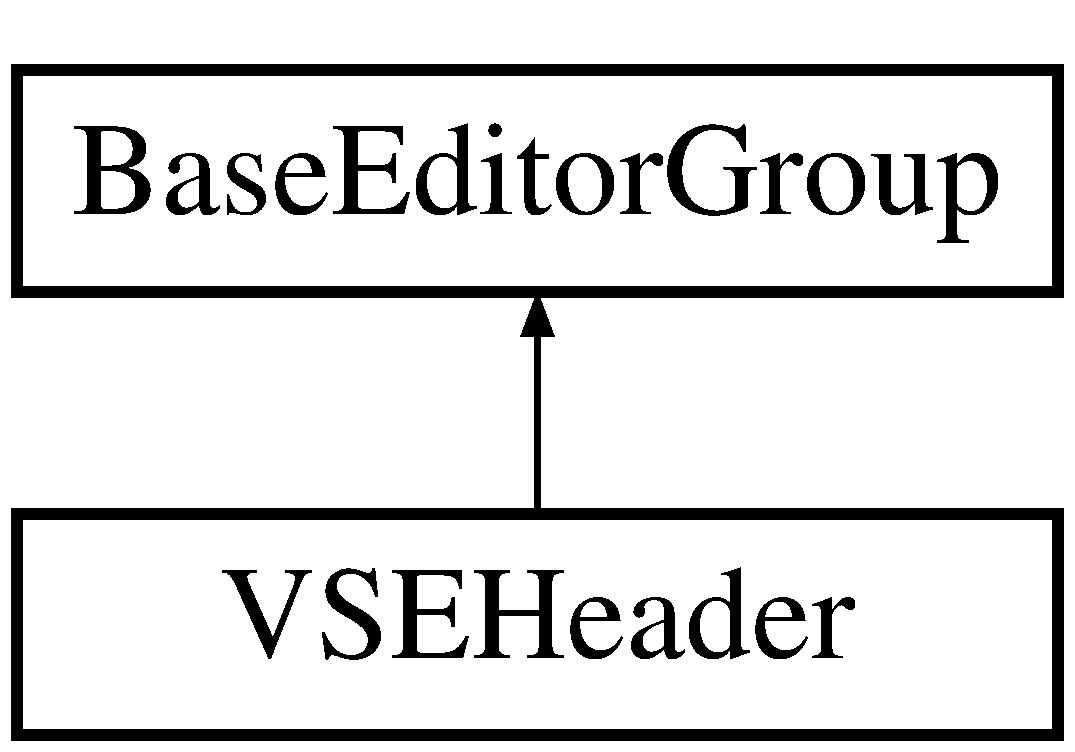
\includegraphics[height=2.000000cm]{class_base_editor_group}
\end{center}
\end{figure}
\subsection*{Public Member Functions}
\begin{DoxyCompactItemize}
\item 
void \hyperlink{class_base_editor_group_a53cc4ec2f041f1d72b0d6468bb930658}{Draw} ()
\begin{DoxyCompactList}\small\item\em Draws the panel itself, not it\textquotesingle{}s content. \end{DoxyCompactList}\item 
virtual void \hyperlink{class_base_editor_group_a8a41e2753ba3c316a1c7fe35ef21897c}{Draw\+Content} ()
\begin{DoxyCompactList}\small\item\em Draws the content of the panel. \end{DoxyCompactList}\item 
virtual void \hyperlink{class_base_editor_group_a2c80ae4df91e93e3d9a1e8e5ea134d7b}{On\+Scene\+UI} (Scene\+View \+\_\+scene\+View)
\begin{DoxyCompactList}\small\item\em Used for drawing in the scene view. \end{DoxyCompactList}\item 
virtual void \hyperlink{class_base_editor_group_a3cd9cee8a3c93fa0c59ad2dac854f367}{Input} (Scene\+View \+\_\+scene\+View)
\begin{DoxyCompactList}\small\item\em Used for handling keyboard input. \end{DoxyCompactList}\item 
virtual void \hyperlink{class_base_editor_group_adaf80fa090e685d7dcd1804f3eac10ca}{Add\+Event\+Listeners} (Scene\+View \+\_\+sceneview)
\begin{DoxyCompactList}\small\item\em Adds the events used in this editor panel. \end{DoxyCompactList}\item 
virtual void \hyperlink{class_base_editor_group_ad584907c5813f11cf979fd9fc80c70c8}{Remove\+Eventlisteners} (Scene\+View \+\_\+sceneview)
\begin{DoxyCompactList}\small\item\em Removes the events used in this editor panel. \end{DoxyCompactList}\end{DoxyCompactItemize}
\subsection*{Public Attributes}
\begin{DoxyCompactItemize}
\item 
Editor\+Window \hyperlink{class_base_editor_group_ac811d2797fc68b5c51f34605228f0672}{parent\+Window}
\begin{DoxyCompactList}\small\item\em The Editor Window this panel is in. \end{DoxyCompactList}\item 
\hyperlink{class_v_m_e_settings_object}{V\+M\+E\+Settings\+Object} \hyperlink{class_base_editor_group_a8915a3a49694f1cfea5a17f9e6bccd16}{settings\+Object}
\begin{DoxyCompactList}\small\item\em Reference to the Object that holds the editor settings. \end{DoxyCompactList}\end{DoxyCompactItemize}


\subsection{Detailed Description}
Base\+Class for a Editor Group. same as Panel but without a toggle state 



\subsection{Member Function Documentation}
\index{Base\+Editor\+Group@{Base\+Editor\+Group}!Add\+Event\+Listeners@{Add\+Event\+Listeners}}
\index{Add\+Event\+Listeners@{Add\+Event\+Listeners}!Base\+Editor\+Group@{Base\+Editor\+Group}}
\subsubsection[{\texorpdfstring{Add\+Event\+Listeners(\+Scene\+View \+\_\+sceneview)}{AddEventListeners(SceneView _sceneview)}}]{\setlength{\rightskip}{0pt plus 5cm}virtual void Base\+Editor\+Group.\+Add\+Event\+Listeners (
\begin{DoxyParamCaption}
\item[{Scene\+View}]{\+\_\+sceneview}
\end{DoxyParamCaption}
)\hspace{0.3cm}{\ttfamily [virtual]}}\hypertarget{class_base_editor_group_adaf80fa090e685d7dcd1804f3eac10ca}{}\label{class_base_editor_group_adaf80fa090e685d7dcd1804f3eac10ca}


Adds the events used in this editor panel. 

\index{Base\+Editor\+Group@{Base\+Editor\+Group}!Draw@{Draw}}
\index{Draw@{Draw}!Base\+Editor\+Group@{Base\+Editor\+Group}}
\subsubsection[{\texorpdfstring{Draw()}{Draw()}}]{\setlength{\rightskip}{0pt plus 5cm}void Base\+Editor\+Group.\+Draw (
\begin{DoxyParamCaption}
{}
\end{DoxyParamCaption}
)}\hypertarget{class_base_editor_group_a53cc4ec2f041f1d72b0d6468bb930658}{}\label{class_base_editor_group_a53cc4ec2f041f1d72b0d6468bb930658}


Draws the panel itself, not it\textquotesingle{}s content. 

\index{Base\+Editor\+Group@{Base\+Editor\+Group}!Draw\+Content@{Draw\+Content}}
\index{Draw\+Content@{Draw\+Content}!Base\+Editor\+Group@{Base\+Editor\+Group}}
\subsubsection[{\texorpdfstring{Draw\+Content()}{DrawContent()}}]{\setlength{\rightskip}{0pt plus 5cm}virtual void Base\+Editor\+Group.\+Draw\+Content (
\begin{DoxyParamCaption}
{}
\end{DoxyParamCaption}
)\hspace{0.3cm}{\ttfamily [virtual]}}\hypertarget{class_base_editor_group_a8a41e2753ba3c316a1c7fe35ef21897c}{}\label{class_base_editor_group_a8a41e2753ba3c316a1c7fe35ef21897c}


Draws the content of the panel. 



Reimplemented in \hyperlink{class_v_s_e_header_ac866415e77168e78f59965f3a61a0e64}{V\+S\+E\+Header}.

\index{Base\+Editor\+Group@{Base\+Editor\+Group}!Input@{Input}}
\index{Input@{Input}!Base\+Editor\+Group@{Base\+Editor\+Group}}
\subsubsection[{\texorpdfstring{Input(\+Scene\+View \+\_\+scene\+View)}{Input(SceneView _sceneView)}}]{\setlength{\rightskip}{0pt plus 5cm}virtual void Base\+Editor\+Group.\+Input (
\begin{DoxyParamCaption}
\item[{Scene\+View}]{\+\_\+scene\+View}
\end{DoxyParamCaption}
)\hspace{0.3cm}{\ttfamily [virtual]}}\hypertarget{class_base_editor_group_a3cd9cee8a3c93fa0c59ad2dac854f367}{}\label{class_base_editor_group_a3cd9cee8a3c93fa0c59ad2dac854f367}


Used for handling keyboard input. 

\index{Base\+Editor\+Group@{Base\+Editor\+Group}!On\+Scene\+UI@{On\+Scene\+UI}}
\index{On\+Scene\+UI@{On\+Scene\+UI}!Base\+Editor\+Group@{Base\+Editor\+Group}}
\subsubsection[{\texorpdfstring{On\+Scene\+U\+I(\+Scene\+View \+\_\+scene\+View)}{OnSceneUI(SceneView _sceneView)}}]{\setlength{\rightskip}{0pt plus 5cm}virtual void Base\+Editor\+Group.\+On\+Scene\+UI (
\begin{DoxyParamCaption}
\item[{Scene\+View}]{\+\_\+scene\+View}
\end{DoxyParamCaption}
)\hspace{0.3cm}{\ttfamily [virtual]}}\hypertarget{class_base_editor_group_a2c80ae4df91e93e3d9a1e8e5ea134d7b}{}\label{class_base_editor_group_a2c80ae4df91e93e3d9a1e8e5ea134d7b}


Used for drawing in the scene view. 

\index{Base\+Editor\+Group@{Base\+Editor\+Group}!Remove\+Eventlisteners@{Remove\+Eventlisteners}}
\index{Remove\+Eventlisteners@{Remove\+Eventlisteners}!Base\+Editor\+Group@{Base\+Editor\+Group}}
\subsubsection[{\texorpdfstring{Remove\+Eventlisteners(\+Scene\+View \+\_\+sceneview)}{RemoveEventlisteners(SceneView _sceneview)}}]{\setlength{\rightskip}{0pt plus 5cm}virtual void Base\+Editor\+Group.\+Remove\+Eventlisteners (
\begin{DoxyParamCaption}
\item[{Scene\+View}]{\+\_\+sceneview}
\end{DoxyParamCaption}
)\hspace{0.3cm}{\ttfamily [virtual]}}\hypertarget{class_base_editor_group_ad584907c5813f11cf979fd9fc80c70c8}{}\label{class_base_editor_group_ad584907c5813f11cf979fd9fc80c70c8}


Removes the events used in this editor panel. 



\subsection{Member Data Documentation}
\index{Base\+Editor\+Group@{Base\+Editor\+Group}!parent\+Window@{parent\+Window}}
\index{parent\+Window@{parent\+Window}!Base\+Editor\+Group@{Base\+Editor\+Group}}
\subsubsection[{\texorpdfstring{parent\+Window}{parentWindow}}]{\setlength{\rightskip}{0pt plus 5cm}Editor\+Window Base\+Editor\+Group.\+parent\+Window}\hypertarget{class_base_editor_group_ac811d2797fc68b5c51f34605228f0672}{}\label{class_base_editor_group_ac811d2797fc68b5c51f34605228f0672}


The Editor Window this panel is in. 

\index{Base\+Editor\+Group@{Base\+Editor\+Group}!settings\+Object@{settings\+Object}}
\index{settings\+Object@{settings\+Object}!Base\+Editor\+Group@{Base\+Editor\+Group}}
\subsubsection[{\texorpdfstring{settings\+Object}{settingsObject}}]{\setlength{\rightskip}{0pt plus 5cm}{\bf V\+M\+E\+Settings\+Object} Base\+Editor\+Group.\+settings\+Object}\hypertarget{class_base_editor_group_a8915a3a49694f1cfea5a17f9e6bccd16}{}\label{class_base_editor_group_a8915a3a49694f1cfea5a17f9e6bccd16}


Reference to the Object that holds the editor settings. 



The documentation for this class was generated from the following file\+:\begin{DoxyCompactItemize}
\item 
C\+:/\+Users/\+Kevin Breurken/\+Documents/\+Projects/\+V\+M\+E/\+Assets/\+V\+M\+E/\+Editor/Base\+Editor\+Group.\+cs\end{DoxyCompactItemize}

\hypertarget{class_base_editor_panel}{}\section{Base\+Editor\+Panel Class Reference}
\label{class_base_editor_panel}\index{Base\+Editor\+Panel@{Base\+Editor\+Panel}}


Base\+Class for a Editor Panel  


Inheritance diagram for Base\+Editor\+Panel\+:\begin{figure}[H]
\begin{center}
\leavevmode
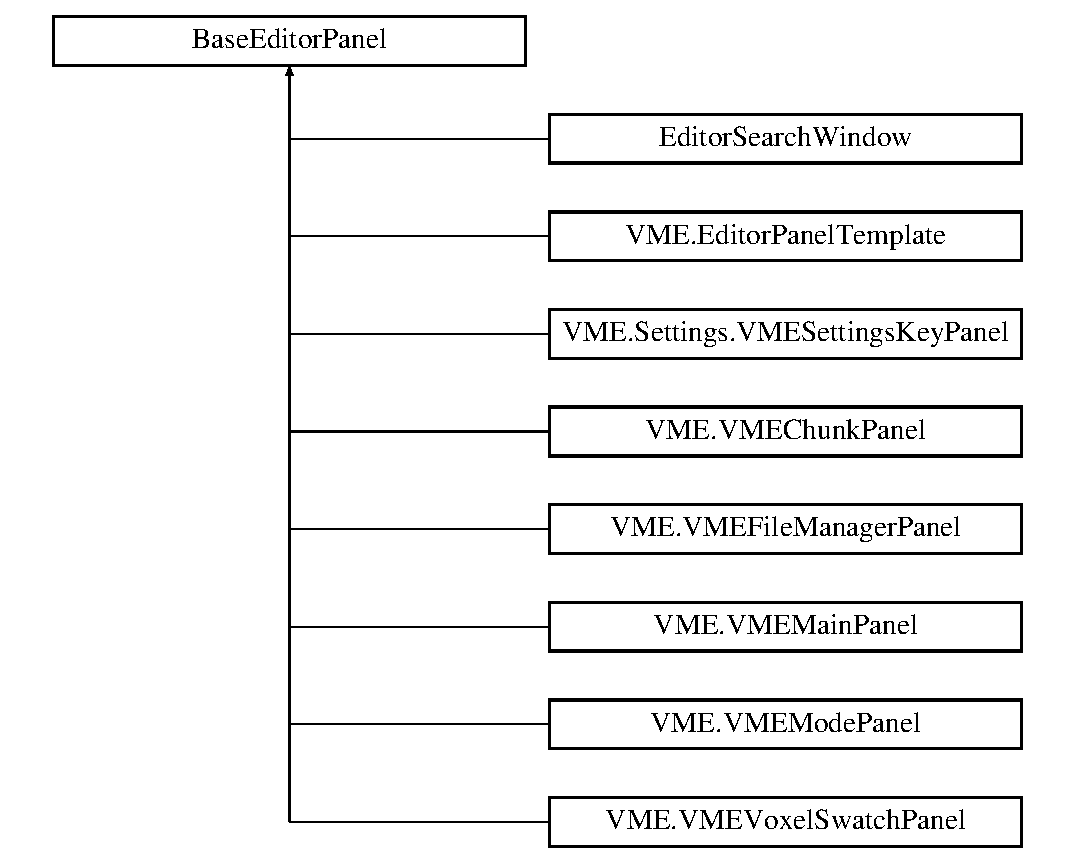
\includegraphics[height=9.000000cm]{class_base_editor_panel}
\end{center}
\end{figure}
\subsection*{Public Member Functions}
\begin{DoxyCompactItemize}
\item 
void \hyperlink{class_base_editor_panel_aa06d39bfb1337b3275d76bf6bc098bbe}{Draw} (string \+\_\+name)
\begin{DoxyCompactList}\small\item\em Draws the panel itself, not it\textquotesingle{}s content. \end{DoxyCompactList}\item 
virtual void \hyperlink{class_base_editor_panel_a96ea35bdda7a8e955baa1fd21635bffa}{Draw\+Content} ()
\begin{DoxyCompactList}\small\item\em Draws the content of the panel. \end{DoxyCompactList}\item 
virtual void \hyperlink{class_base_editor_panel_a3a8ccb88e5e34920880e9000a48fb862}{On\+Opened} ()
\begin{DoxyCompactList}\small\item\em Called when the panel is opened. \end{DoxyCompactList}\item 
virtual void \hyperlink{class_base_editor_panel_a88a1951ff16bc1aa4534fb768c0a7c59}{On\+Closed} ()
\begin{DoxyCompactList}\small\item\em Called when the panel is closed. \end{DoxyCompactList}\item 
virtual void \hyperlink{class_base_editor_panel_a720cd4b21ce5c74b52ba310d9978e6e3}{On\+Scene\+UI} (Scene\+View \+\_\+scene\+View)
\begin{DoxyCompactList}\small\item\em Used for drawing in the scene view. \end{DoxyCompactList}\item 
virtual void \hyperlink{class_base_editor_panel_a9bd01437be0e246418dc89209ef2125b}{Input} (Scene\+View \+\_\+scene\+View)
\begin{DoxyCompactList}\small\item\em Used for handling keyboard input. \end{DoxyCompactList}\item 
void \hyperlink{class_base_editor_panel_ae58c401d801f1b987c5314a9195d8f2c}{Check\+Panel\+State} ()
\begin{DoxyCompactList}\small\item\em Checks if the window state is changed. \end{DoxyCompactList}\item 
virtual void \hyperlink{class_base_editor_panel_ac35cb29ff5d4e06dde071f7e1b16629d}{Add\+Event\+Listeners} (Scene\+View \+\_\+sceneview)
\begin{DoxyCompactList}\small\item\em Adds the events used in this editor panel. \end{DoxyCompactList}\item 
virtual void \hyperlink{class_base_editor_panel_a18cb314bcfdc5b56bfc0dcd316023bb6}{Remove\+Eventlisteners} (Scene\+View \+\_\+sceneview)
\begin{DoxyCompactList}\small\item\em Removes the events used in this editor panel. \end{DoxyCompactList}\item 
void \hyperlink{class_base_editor_panel_a6aa206595fa39c904d248dc6bd9fb8b9}{Set\+State} (bool \+\_\+state)
\begin{DoxyCompactList}\small\item\em Sets the current state of the panel. \end{DoxyCompactList}\end{DoxyCompactItemize}
\subsection*{Public Attributes}
\begin{DoxyCompactItemize}
\item 
bool \hyperlink{class_base_editor_panel_ab42b67df97ab6bb60248f925668e4716}{is\+Open} = false
\begin{DoxyCompactList}\small\item\em if the panel is currently opened. \end{DoxyCompactList}\item 
Key\+Code \hyperlink{class_base_editor_panel_af34e3c07554a0c56901e6c9c6fe4d33c}{toggle\+Key}
\begin{DoxyCompactList}\small\item\em Key used for activating this panel. \end{DoxyCompactList}\item 
Editor\+Window \hyperlink{class_base_editor_panel_a9b10134d16fca13b5c9b400ccbd06543}{parent\+Window}
\begin{DoxyCompactList}\small\item\em The Editor Window this panel is in. \end{DoxyCompactList}\item 
\hyperlink{class_v_m_e_settings_object}{V\+M\+E\+Settings\+Object} \hyperlink{class_base_editor_panel_a4b4881caa31e3604aaaa5f6914405e8a}{settings\+Object}
\begin{DoxyCompactList}\small\item\em Reference to the Object that holds the editor settings. \end{DoxyCompactList}\end{DoxyCompactItemize}


\subsection{Detailed Description}
Base\+Class for a Editor Panel 



\subsection{Member Function Documentation}
\index{Base\+Editor\+Panel@{Base\+Editor\+Panel}!Add\+Event\+Listeners@{Add\+Event\+Listeners}}
\index{Add\+Event\+Listeners@{Add\+Event\+Listeners}!Base\+Editor\+Panel@{Base\+Editor\+Panel}}
\subsubsection[{\texorpdfstring{Add\+Event\+Listeners(\+Scene\+View \+\_\+sceneview)}{AddEventListeners(SceneView _sceneview)}}]{\setlength{\rightskip}{0pt plus 5cm}virtual void Base\+Editor\+Panel.\+Add\+Event\+Listeners (
\begin{DoxyParamCaption}
\item[{Scene\+View}]{\+\_\+sceneview}
\end{DoxyParamCaption}
)\hspace{0.3cm}{\ttfamily [virtual]}}\hypertarget{class_base_editor_panel_ac35cb29ff5d4e06dde071f7e1b16629d}{}\label{class_base_editor_panel_ac35cb29ff5d4e06dde071f7e1b16629d}


Adds the events used in this editor panel. 

\index{Base\+Editor\+Panel@{Base\+Editor\+Panel}!Check\+Panel\+State@{Check\+Panel\+State}}
\index{Check\+Panel\+State@{Check\+Panel\+State}!Base\+Editor\+Panel@{Base\+Editor\+Panel}}
\subsubsection[{\texorpdfstring{Check\+Panel\+State()}{CheckPanelState()}}]{\setlength{\rightskip}{0pt plus 5cm}void Base\+Editor\+Panel.\+Check\+Panel\+State (
\begin{DoxyParamCaption}
{}
\end{DoxyParamCaption}
)}\hypertarget{class_base_editor_panel_ae58c401d801f1b987c5314a9195d8f2c}{}\label{class_base_editor_panel_ae58c401d801f1b987c5314a9195d8f2c}


Checks if the window state is changed. 

\index{Base\+Editor\+Panel@{Base\+Editor\+Panel}!Draw@{Draw}}
\index{Draw@{Draw}!Base\+Editor\+Panel@{Base\+Editor\+Panel}}
\subsubsection[{\texorpdfstring{Draw(string \+\_\+name)}{Draw(string _name)}}]{\setlength{\rightskip}{0pt plus 5cm}void Base\+Editor\+Panel.\+Draw (
\begin{DoxyParamCaption}
\item[{string}]{\+\_\+name}
\end{DoxyParamCaption}
)}\hypertarget{class_base_editor_panel_aa06d39bfb1337b3275d76bf6bc098bbe}{}\label{class_base_editor_panel_aa06d39bfb1337b3275d76bf6bc098bbe}


Draws the panel itself, not it\textquotesingle{}s content. 

\index{Base\+Editor\+Panel@{Base\+Editor\+Panel}!Draw\+Content@{Draw\+Content}}
\index{Draw\+Content@{Draw\+Content}!Base\+Editor\+Panel@{Base\+Editor\+Panel}}
\subsubsection[{\texorpdfstring{Draw\+Content()}{DrawContent()}}]{\setlength{\rightskip}{0pt plus 5cm}virtual void Base\+Editor\+Panel.\+Draw\+Content (
\begin{DoxyParamCaption}
{}
\end{DoxyParamCaption}
)\hspace{0.3cm}{\ttfamily [virtual]}}\hypertarget{class_base_editor_panel_a96ea35bdda7a8e955baa1fd21635bffa}{}\label{class_base_editor_panel_a96ea35bdda7a8e955baa1fd21635bffa}


Draws the content of the panel. 



Reimplemented in \hyperlink{class_v_m_e_1_1_v_m_e_chunk_panel_a40223de4b7a04a2dc23a65fc57bfa387}{V\+M\+E.\+V\+M\+E\+Chunk\+Panel}, \hyperlink{class_v_m_e_1_1_v_m_e_mode_panel_ab60ed5d8ad208884843eb77a0633986d}{V\+M\+E.\+V\+M\+E\+Mode\+Panel}, \hyperlink{class_v_m_e_1_1_v_m_e_voxel_swatch_panel_a663cd8478cdcb41c20fc9078f893c3a0}{V\+M\+E.\+V\+M\+E\+Voxel\+Swatch\+Panel}, \hyperlink{class_editor_search_window_a31b2db7b66d3e97910ec8ad403b55a6a}{Editor\+Search\+Window}, \hyperlink{class_v_m_e_1_1_v_m_e_main_panel_a31c00f8725239c4e1758f32bb0d29cf9}{V\+M\+E.\+V\+M\+E\+Main\+Panel}, \hyperlink{class_v_m_e_1_1_v_m_e_file_manager_panel_a328194babcf088ee2e1a4ab89deeb916}{V\+M\+E.\+V\+M\+E\+File\+Manager\+Panel}, \hyperlink{class_v_m_e_1_1_editor_panel_template_ad7ea6c92ea74e7482000cb1cfe4617a3}{V\+M\+E.\+Editor\+Panel\+Template}, and \hyperlink{class_v_m_e_1_1_settings_1_1_v_m_e_settings_key_panel_a37a1629cea9d0dedcc887d52d54b036c}{V\+M\+E.\+Settings.\+V\+M\+E\+Settings\+Key\+Panel}.

\index{Base\+Editor\+Panel@{Base\+Editor\+Panel}!Input@{Input}}
\index{Input@{Input}!Base\+Editor\+Panel@{Base\+Editor\+Panel}}
\subsubsection[{\texorpdfstring{Input(\+Scene\+View \+\_\+scene\+View)}{Input(SceneView _sceneView)}}]{\setlength{\rightskip}{0pt plus 5cm}virtual void Base\+Editor\+Panel.\+Input (
\begin{DoxyParamCaption}
\item[{Scene\+View}]{\+\_\+scene\+View}
\end{DoxyParamCaption}
)\hspace{0.3cm}{\ttfamily [virtual]}}\hypertarget{class_base_editor_panel_a9bd01437be0e246418dc89209ef2125b}{}\label{class_base_editor_panel_a9bd01437be0e246418dc89209ef2125b}


Used for handling keyboard input. 



Reimplemented in \hyperlink{class_editor_search_window_a7eae97a116499dd637254664c1cf3b81}{Editor\+Search\+Window}, \hyperlink{class_v_m_e_1_1_v_m_e_voxel_swatch_panel_a4c94c74221d96e48ed17ecb6b2a98ffb}{V\+M\+E.\+V\+M\+E\+Voxel\+Swatch\+Panel}, \hyperlink{class_v_m_e_1_1_v_m_e_mode_panel_adef41bb2208966390ef8557311fd576f}{V\+M\+E.\+V\+M\+E\+Mode\+Panel}, \hyperlink{class_v_m_e_1_1_v_m_e_file_manager_panel_ac39bb43df82776379e2f31c67b0ced93}{V\+M\+E.\+V\+M\+E\+File\+Manager\+Panel}, \hyperlink{class_v_m_e_1_1_v_m_e_main_panel_a3ee8bf67ac932165d48986d3dbba1fb4}{V\+M\+E.\+V\+M\+E\+Main\+Panel}, and \hyperlink{class_v_m_e_1_1_editor_panel_template_a816b7994b28d7ac4ae3ccd1ebbccf675}{V\+M\+E.\+Editor\+Panel\+Template}.

\index{Base\+Editor\+Panel@{Base\+Editor\+Panel}!On\+Closed@{On\+Closed}}
\index{On\+Closed@{On\+Closed}!Base\+Editor\+Panel@{Base\+Editor\+Panel}}
\subsubsection[{\texorpdfstring{On\+Closed()}{OnClosed()}}]{\setlength{\rightskip}{0pt plus 5cm}virtual void Base\+Editor\+Panel.\+On\+Closed (
\begin{DoxyParamCaption}
{}
\end{DoxyParamCaption}
)\hspace{0.3cm}{\ttfamily [virtual]}}\hypertarget{class_base_editor_panel_a88a1951ff16bc1aa4534fb768c0a7c59}{}\label{class_base_editor_panel_a88a1951ff16bc1aa4534fb768c0a7c59}


Called when the panel is closed. 

\index{Base\+Editor\+Panel@{Base\+Editor\+Panel}!On\+Opened@{On\+Opened}}
\index{On\+Opened@{On\+Opened}!Base\+Editor\+Panel@{Base\+Editor\+Panel}}
\subsubsection[{\texorpdfstring{On\+Opened()}{OnOpened()}}]{\setlength{\rightskip}{0pt plus 5cm}virtual void Base\+Editor\+Panel.\+On\+Opened (
\begin{DoxyParamCaption}
{}
\end{DoxyParamCaption}
)\hspace{0.3cm}{\ttfamily [virtual]}}\hypertarget{class_base_editor_panel_a3a8ccb88e5e34920880e9000a48fb862}{}\label{class_base_editor_panel_a3a8ccb88e5e34920880e9000a48fb862}


Called when the panel is opened. 



Reimplemented in \hyperlink{class_v_m_e_1_1_v_m_e_chunk_panel_a61ffdb0c341b6571f8193a2c4caefb0e}{V\+M\+E.\+V\+M\+E\+Chunk\+Panel}, and \hyperlink{class_v_m_e_1_1_v_m_e_voxel_swatch_panel_a1756e7e5d376e59d966b26d21c9e9d3c}{V\+M\+E.\+V\+M\+E\+Voxel\+Swatch\+Panel}.

\index{Base\+Editor\+Panel@{Base\+Editor\+Panel}!On\+Scene\+UI@{On\+Scene\+UI}}
\index{On\+Scene\+UI@{On\+Scene\+UI}!Base\+Editor\+Panel@{Base\+Editor\+Panel}}
\subsubsection[{\texorpdfstring{On\+Scene\+U\+I(\+Scene\+View \+\_\+scene\+View)}{OnSceneUI(SceneView _sceneView)}}]{\setlength{\rightskip}{0pt plus 5cm}virtual void Base\+Editor\+Panel.\+On\+Scene\+UI (
\begin{DoxyParamCaption}
\item[{Scene\+View}]{\+\_\+scene\+View}
\end{DoxyParamCaption}
)\hspace{0.3cm}{\ttfamily [virtual]}}\hypertarget{class_base_editor_panel_a720cd4b21ce5c74b52ba310d9978e6e3}{}\label{class_base_editor_panel_a720cd4b21ce5c74b52ba310d9978e6e3}


Used for drawing in the scene view. 



Reimplemented in \hyperlink{class_v_m_e_1_1_v_m_e_mode_panel_a20fc99c3b9d0dc77b0b8bd72ed070177}{V\+M\+E.\+V\+M\+E\+Mode\+Panel}.

\index{Base\+Editor\+Panel@{Base\+Editor\+Panel}!Remove\+Eventlisteners@{Remove\+Eventlisteners}}
\index{Remove\+Eventlisteners@{Remove\+Eventlisteners}!Base\+Editor\+Panel@{Base\+Editor\+Panel}}
\subsubsection[{\texorpdfstring{Remove\+Eventlisteners(\+Scene\+View \+\_\+sceneview)}{RemoveEventlisteners(SceneView _sceneview)}}]{\setlength{\rightskip}{0pt plus 5cm}virtual void Base\+Editor\+Panel.\+Remove\+Eventlisteners (
\begin{DoxyParamCaption}
\item[{Scene\+View}]{\+\_\+sceneview}
\end{DoxyParamCaption}
)\hspace{0.3cm}{\ttfamily [virtual]}}\hypertarget{class_base_editor_panel_a18cb314bcfdc5b56bfc0dcd316023bb6}{}\label{class_base_editor_panel_a18cb314bcfdc5b56bfc0dcd316023bb6}


Removes the events used in this editor panel. 

\index{Base\+Editor\+Panel@{Base\+Editor\+Panel}!Set\+State@{Set\+State}}
\index{Set\+State@{Set\+State}!Base\+Editor\+Panel@{Base\+Editor\+Panel}}
\subsubsection[{\texorpdfstring{Set\+State(bool \+\_\+state)}{SetState(bool _state)}}]{\setlength{\rightskip}{0pt plus 5cm}void Base\+Editor\+Panel.\+Set\+State (
\begin{DoxyParamCaption}
\item[{bool}]{\+\_\+state}
\end{DoxyParamCaption}
)}\hypertarget{class_base_editor_panel_a6aa206595fa39c904d248dc6bd9fb8b9}{}\label{class_base_editor_panel_a6aa206595fa39c904d248dc6bd9fb8b9}


Sets the current state of the panel. 



\subsection{Member Data Documentation}
\index{Base\+Editor\+Panel@{Base\+Editor\+Panel}!is\+Open@{is\+Open}}
\index{is\+Open@{is\+Open}!Base\+Editor\+Panel@{Base\+Editor\+Panel}}
\subsubsection[{\texorpdfstring{is\+Open}{isOpen}}]{\setlength{\rightskip}{0pt plus 5cm}bool Base\+Editor\+Panel.\+is\+Open = false}\hypertarget{class_base_editor_panel_ab42b67df97ab6bb60248f925668e4716}{}\label{class_base_editor_panel_ab42b67df97ab6bb60248f925668e4716}


if the panel is currently opened. 

\index{Base\+Editor\+Panel@{Base\+Editor\+Panel}!parent\+Window@{parent\+Window}}
\index{parent\+Window@{parent\+Window}!Base\+Editor\+Panel@{Base\+Editor\+Panel}}
\subsubsection[{\texorpdfstring{parent\+Window}{parentWindow}}]{\setlength{\rightskip}{0pt plus 5cm}Editor\+Window Base\+Editor\+Panel.\+parent\+Window}\hypertarget{class_base_editor_panel_a9b10134d16fca13b5c9b400ccbd06543}{}\label{class_base_editor_panel_a9b10134d16fca13b5c9b400ccbd06543}


The Editor Window this panel is in. 

\index{Base\+Editor\+Panel@{Base\+Editor\+Panel}!settings\+Object@{settings\+Object}}
\index{settings\+Object@{settings\+Object}!Base\+Editor\+Panel@{Base\+Editor\+Panel}}
\subsubsection[{\texorpdfstring{settings\+Object}{settingsObject}}]{\setlength{\rightskip}{0pt plus 5cm}{\bf V\+M\+E\+Settings\+Object} Base\+Editor\+Panel.\+settings\+Object}\hypertarget{class_base_editor_panel_a4b4881caa31e3604aaaa5f6914405e8a}{}\label{class_base_editor_panel_a4b4881caa31e3604aaaa5f6914405e8a}


Reference to the Object that holds the editor settings. 

\index{Base\+Editor\+Panel@{Base\+Editor\+Panel}!toggle\+Key@{toggle\+Key}}
\index{toggle\+Key@{toggle\+Key}!Base\+Editor\+Panel@{Base\+Editor\+Panel}}
\subsubsection[{\texorpdfstring{toggle\+Key}{toggleKey}}]{\setlength{\rightskip}{0pt plus 5cm}Key\+Code Base\+Editor\+Panel.\+toggle\+Key}\hypertarget{class_base_editor_panel_af34e3c07554a0c56901e6c9c6fe4d33c}{}\label{class_base_editor_panel_af34e3c07554a0c56901e6c9c6fe4d33c}


Key used for activating this panel. 



The documentation for this class was generated from the following file\+:\begin{DoxyCompactItemize}
\item 
C\+:/\+Users/\+Kevin Breurken/\+Documents/\+Projects/\+V\+M\+E/\+Assets/\+V\+M\+E/\+Editor/Base\+Editor\+Panel.\+cs\end{DoxyCompactItemize}

\hypertarget{class_chunk}{}\section{Chunk Class Reference}
\label{class_chunk}\index{Chunk@{Chunk}}
Inheritance diagram for Chunk\+:\begin{figure}[H]
\begin{center}
\leavevmode
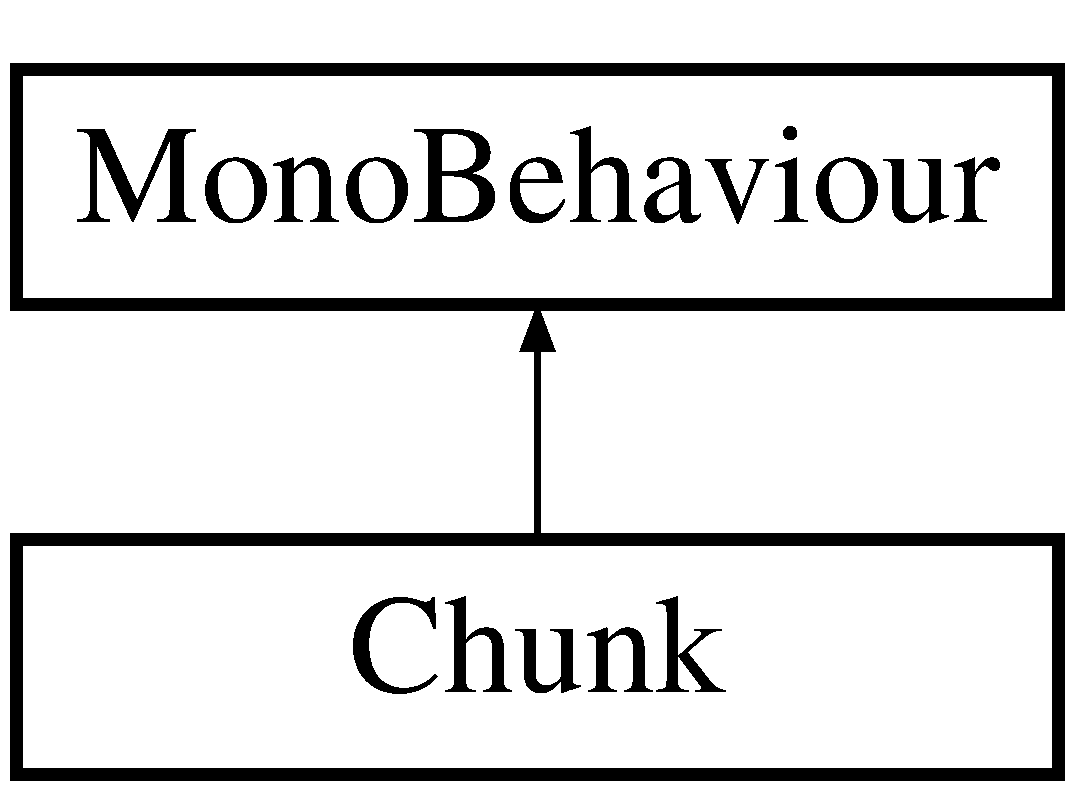
\includegraphics[height=2.000000cm]{class_chunk}
\end{center}
\end{figure}
\subsection*{Public Attributes}
\begin{DoxyCompactItemize}
\item 
bool {\bfseries drawbounds}\hypertarget{class_chunk_aa46dfc546e0e24f2a8a0444baef51bba}{}\label{class_chunk_aa46dfc546e0e24f2a8a0444baef51bba}

\item 
Transform {\bfseries Tile\+Layer}\hypertarget{class_chunk_ab506fb9adf7c1dc3de9421dec3187fa5}{}\label{class_chunk_ab506fb9adf7c1dc3de9421dec3187fa5}

\item 
Transform {\bfseries Props\+Layer}\hypertarget{class_chunk_a40fe7f30cc1a82fcddb772ad528c8f3e}{}\label{class_chunk_a40fe7f30cc1a82fcddb772ad528c8f3e}

\item 
Transform {\bfseries Interactive\+Layer}\hypertarget{class_chunk_af3445842a83849116e7cd9d7484c0e76}{}\label{class_chunk_af3445842a83849116e7cd9d7484c0e76}

\item 
Transform {\bfseries Effect\+Layer}\hypertarget{class_chunk_a6e1204c82272a460e0ad1b9a6a3bb299}{}\label{class_chunk_a6e1204c82272a460e0ad1b9a6a3bb299}

\end{DoxyCompactItemize}


The documentation for this class was generated from the following file\+:\begin{DoxyCompactItemize}
\item 
C\+:/\+Users/\+Kevin Breurken/\+Documents/\+Projects/\+V\+M\+E/\+Assets/\+V\+M\+E/\+Scripts/Chunk.\+cs\end{DoxyCompactItemize}

\hypertarget{class_chunk_object_data}{}\section{Chunk\+Object\+Data Class Reference}
\label{class_chunk_object_data}\index{Chunk\+Object\+Data@{Chunk\+Object\+Data}}
Inheritance diagram for Chunk\+Object\+Data\+:\begin{figure}[H]
\begin{center}
\leavevmode
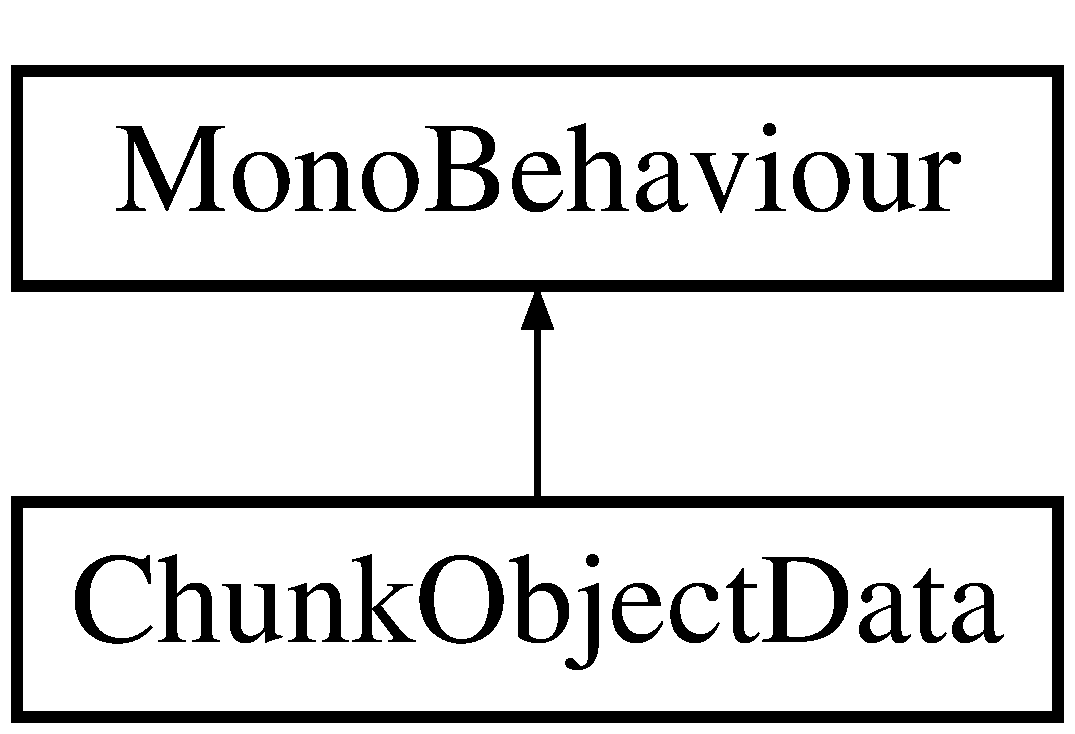
\includegraphics[height=2.000000cm]{class_chunk_object_data}
\end{center}
\end{figure}
\subsection*{Public Attributes}
\begin{DoxyCompactItemize}
\item 
bool {\bfseries has\+Collider}\hypertarget{class_chunk_object_data_a8e898a50778de2f10b16ef1278d0503d}{}\label{class_chunk_object_data_a8e898a50778de2f10b16ef1278d0503d}

\end{DoxyCompactItemize}


The documentation for this class was generated from the following file\+:\begin{DoxyCompactItemize}
\item 
C\+:/\+Users/\+Kevin Breurken/\+Documents/\+Projects/\+V\+M\+E/\+Assets/\+V\+M\+E/\+Scripts/Chunk\+Object\+Data.\+cs\end{DoxyCompactItemize}

\hypertarget{class_chunk_spawner}{}\section{Chunk\+Spawner Class Reference}
\label{class_chunk_spawner}\index{Chunk\+Spawner@{Chunk\+Spawner}}


Spawn chunk inside the editor, and save it.  


Inheritance diagram for Chunk\+Spawner\+:\begin{figure}[H]
\begin{center}
\leavevmode
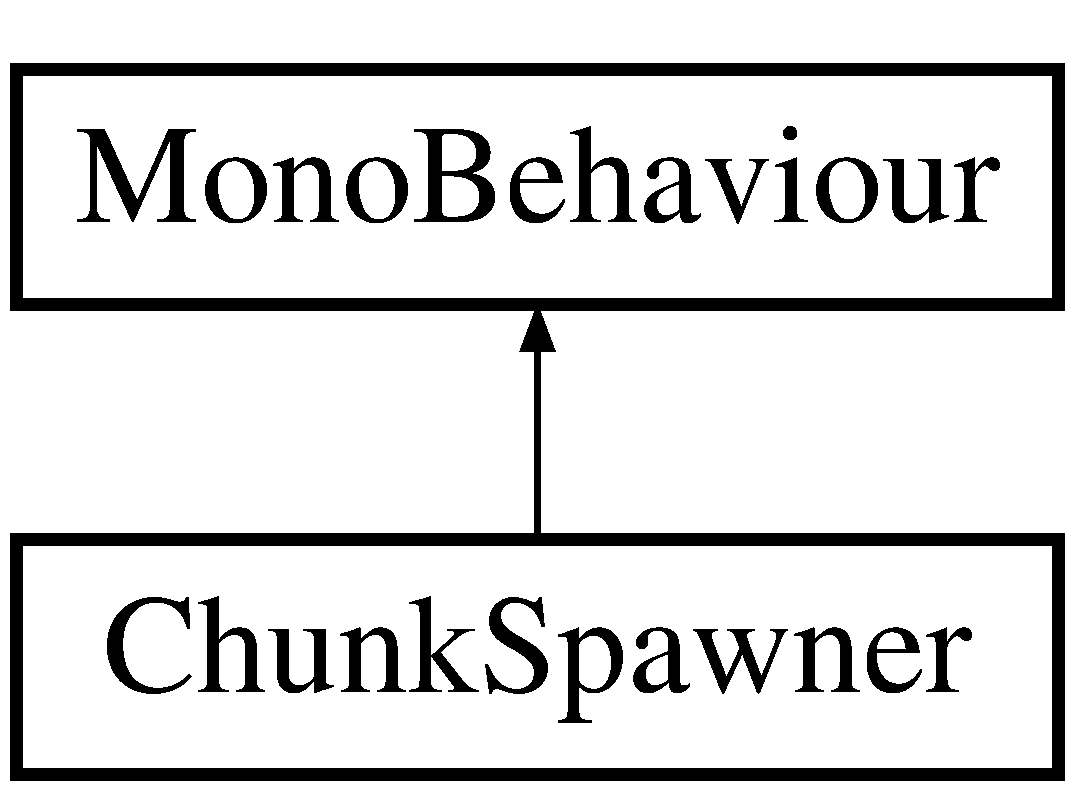
\includegraphics[height=2.000000cm]{class_chunk_spawner}
\end{center}
\end{figure}
\subsection*{Public Member Functions}
\begin{DoxyCompactItemize}
\item 
void {\bfseries Load} ()\hypertarget{class_chunk_spawner_ac03ab97765bb71f200f6e39cdd92a25c}{}\label{class_chunk_spawner_ac03ab97765bb71f200f6e39cdd92a25c}

\item 
void {\bfseries Unload} ()\hypertarget{class_chunk_spawner_a629ab03d88a4479bdf85258cb679eff8}{}\label{class_chunk_spawner_a629ab03d88a4479bdf85258cb679eff8}

\end{DoxyCompactItemize}
\subsection*{Public Attributes}
\begin{DoxyCompactItemize}
\item 
\hyperlink{class_chunk}{Chunk} {\bfseries chunk}\hypertarget{class_chunk_spawner_a3851a334ae9f006109b37513b5211f81}{}\label{class_chunk_spawner_a3851a334ae9f006109b37513b5211f81}

\end{DoxyCompactItemize}


\subsection{Detailed Description}
Spawn chunk inside the editor, and save it. 



The documentation for this class was generated from the following file\+:\begin{DoxyCompactItemize}
\item 
C\+:/\+Users/\+Kevin Breurken/\+Documents/\+Projects/\+V\+M\+E/\+Assets/\+V\+M\+E/\+Scripts/Chunk\+Spawner.\+cs\end{DoxyCompactItemize}

\hypertarget{class_editor_u_i_1_1_draw}{}\section{Editor\+U\+I.\+Draw Class Reference}
\label{class_editor_u_i_1_1_draw}\index{Editor\+U\+I.\+Draw@{Editor\+U\+I.\+Draw}}


Fancier UI functions.  


\subsection*{Static Public Member Functions}
\begin{DoxyCompactItemize}
\item 
static void \hyperlink{class_editor_u_i_1_1_draw_ab4ae9edd7ae1195156451f3691a7c05d}{Title\+Field} (string text)
\begin{DoxyCompactList}\small\item\em Draws a Title \end{DoxyCompactList}\item 
static void \hyperlink{class_editor_u_i_1_1_draw_ad0f352e4d2d341ced1852d44224d46a5}{Pressed\+Button} (string text)
\begin{DoxyCompactList}\small\item\em Draws a Pressed in Button \end{DoxyCompactList}\end{DoxyCompactItemize}


\subsection{Detailed Description}
Fancier UI functions. 



\subsection{Member Function Documentation}
\index{Editor\+U\+I\+::\+Draw@{Editor\+U\+I\+::\+Draw}!Pressed\+Button@{Pressed\+Button}}
\index{Pressed\+Button@{Pressed\+Button}!Editor\+U\+I\+::\+Draw@{Editor\+U\+I\+::\+Draw}}
\subsubsection[{\texorpdfstring{Pressed\+Button(string text)}{PressedButton(string text)}}]{\setlength{\rightskip}{0pt plus 5cm}static void Editor\+U\+I.\+Draw.\+Pressed\+Button (
\begin{DoxyParamCaption}
\item[{string}]{text}
\end{DoxyParamCaption}
)\hspace{0.3cm}{\ttfamily [static]}}\hypertarget{class_editor_u_i_1_1_draw_ad0f352e4d2d341ced1852d44224d46a5}{}\label{class_editor_u_i_1_1_draw_ad0f352e4d2d341ced1852d44224d46a5}


Draws a Pressed in Button 

\index{Editor\+U\+I\+::\+Draw@{Editor\+U\+I\+::\+Draw}!Title\+Field@{Title\+Field}}
\index{Title\+Field@{Title\+Field}!Editor\+U\+I\+::\+Draw@{Editor\+U\+I\+::\+Draw}}
\subsubsection[{\texorpdfstring{Title\+Field(string text)}{TitleField(string text)}}]{\setlength{\rightskip}{0pt plus 5cm}static void Editor\+U\+I.\+Draw.\+Title\+Field (
\begin{DoxyParamCaption}
\item[{string}]{text}
\end{DoxyParamCaption}
)\hspace{0.3cm}{\ttfamily [static]}}\hypertarget{class_editor_u_i_1_1_draw_ab4ae9edd7ae1195156451f3691a7c05d}{}\label{class_editor_u_i_1_1_draw_ab4ae9edd7ae1195156451f3691a7c05d}


Draws a Title 



The documentation for this class was generated from the following file\+:\begin{DoxyCompactItemize}
\item 
C\+:/\+Users/\+Kevin Breurken/\+Documents/\+Projects/\+V\+M\+E/\+Assets/\+V\+M\+E/\+Editor/Editor\+U\+I.\+cs\end{DoxyCompactItemize}

\hypertarget{class_v_m_e_1_1_editor_panel_template}{}\section{V\+M\+E.\+Editor\+Panel\+Template Class Reference}
\label{class_v_m_e_1_1_editor_panel_template}\index{V\+M\+E.\+Editor\+Panel\+Template@{V\+M\+E.\+Editor\+Panel\+Template}}
Inheritance diagram for V\+M\+E.\+Editor\+Panel\+Template\+:\begin{figure}[H]
\begin{center}
\leavevmode
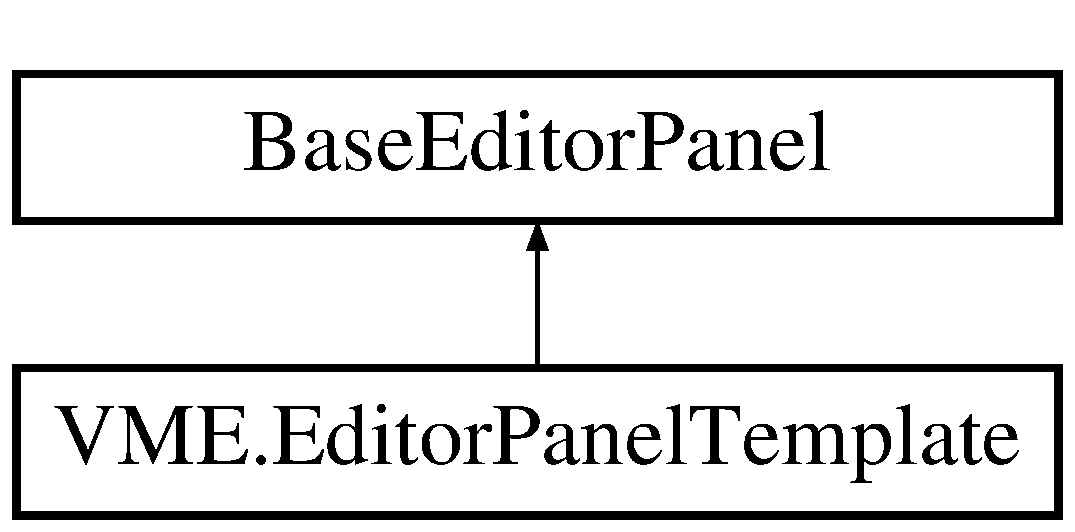
\includegraphics[height=2.000000cm]{class_v_m_e_1_1_editor_panel_template}
\end{center}
\end{figure}
\subsection*{Public Member Functions}
\begin{DoxyCompactItemize}
\item 
{\bfseries Editor\+Panel\+Template} (Editor\+Window \+\_\+window, Key\+Code \+\_\+toggle\+Key)\hypertarget{class_v_m_e_1_1_editor_panel_template_aea32ee297d08364f9a9a8f3a04907ee9}{}\label{class_v_m_e_1_1_editor_panel_template_aea32ee297d08364f9a9a8f3a04907ee9}

\item 
override void \hyperlink{class_v_m_e_1_1_editor_panel_template_ad7ea6c92ea74e7482000cb1cfe4617a3}{Draw\+Content} ()
\begin{DoxyCompactList}\small\item\em Draws the content of the panel. \end{DoxyCompactList}\item 
override void \hyperlink{class_v_m_e_1_1_editor_panel_template_a816b7994b28d7ac4ae3ccd1ebbccf675}{Input} (Scene\+View scene\+View)
\begin{DoxyCompactList}\small\item\em Used for handling keyboard input. \end{DoxyCompactList}\end{DoxyCompactItemize}
\subsection*{Additional Inherited Members}


\subsection{Member Function Documentation}
\index{V\+M\+E\+::\+Editor\+Panel\+Template@{V\+M\+E\+::\+Editor\+Panel\+Template}!Draw\+Content@{Draw\+Content}}
\index{Draw\+Content@{Draw\+Content}!V\+M\+E\+::\+Editor\+Panel\+Template@{V\+M\+E\+::\+Editor\+Panel\+Template}}
\subsubsection[{\texorpdfstring{Draw\+Content()}{DrawContent()}}]{\setlength{\rightskip}{0pt plus 5cm}override void V\+M\+E.\+Editor\+Panel\+Template.\+Draw\+Content (
\begin{DoxyParamCaption}
{}
\end{DoxyParamCaption}
)\hspace{0.3cm}{\ttfamily [virtual]}}\hypertarget{class_v_m_e_1_1_editor_panel_template_ad7ea6c92ea74e7482000cb1cfe4617a3}{}\label{class_v_m_e_1_1_editor_panel_template_ad7ea6c92ea74e7482000cb1cfe4617a3}


Draws the content of the panel. 



Reimplemented from \hyperlink{class_base_editor_panel_a96ea35bdda7a8e955baa1fd21635bffa}{Base\+Editor\+Panel}.

\index{V\+M\+E\+::\+Editor\+Panel\+Template@{V\+M\+E\+::\+Editor\+Panel\+Template}!Input@{Input}}
\index{Input@{Input}!V\+M\+E\+::\+Editor\+Panel\+Template@{V\+M\+E\+::\+Editor\+Panel\+Template}}
\subsubsection[{\texorpdfstring{Input(\+Scene\+View scene\+View)}{Input(SceneView sceneView)}}]{\setlength{\rightskip}{0pt plus 5cm}override void V\+M\+E.\+Editor\+Panel\+Template.\+Input (
\begin{DoxyParamCaption}
\item[{Scene\+View}]{\+\_\+scene\+View}
\end{DoxyParamCaption}
)\hspace{0.3cm}{\ttfamily [virtual]}}\hypertarget{class_v_m_e_1_1_editor_panel_template_a816b7994b28d7ac4ae3ccd1ebbccf675}{}\label{class_v_m_e_1_1_editor_panel_template_a816b7994b28d7ac4ae3ccd1ebbccf675}


Used for handling keyboard input. 



Reimplemented from \hyperlink{class_base_editor_panel_a9bd01437be0e246418dc89209ef2125b}{Base\+Editor\+Panel}.



The documentation for this class was generated from the following file\+:\begin{DoxyCompactItemize}
\item 
C\+:/\+Users/\+Kevin Breurken/\+Documents/\+Projects/\+V\+M\+E/\+Assets/\+V\+M\+E/\+Editor/\+Other/Editor\+Panel\+Template.\+cs\end{DoxyCompactItemize}

\hypertarget{class_editor_search_window}{}\section{Editor\+Search\+Window Class Reference}
\label{class_editor_search_window}\index{Editor\+Search\+Window@{Editor\+Search\+Window}}
Inheritance diagram for Editor\+Search\+Window\+:\begin{figure}[H]
\begin{center}
\leavevmode
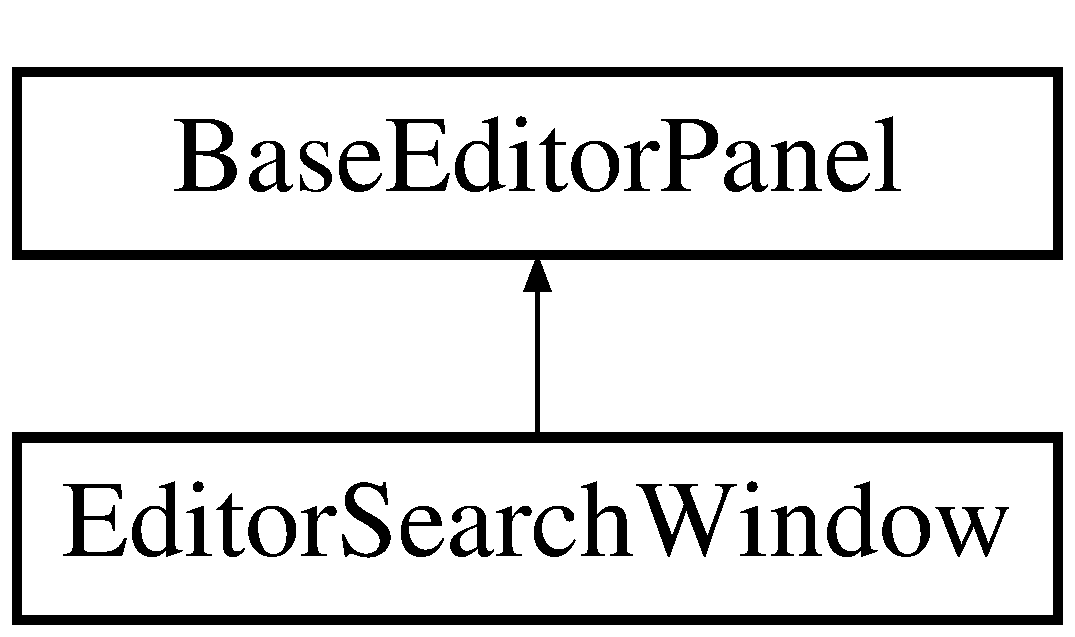
\includegraphics[height=2.000000cm]{class_editor_search_window}
\end{center}
\end{figure}
\subsection*{Public Member Functions}
\begin{DoxyCompactItemize}
\item 
delegate void {\bfseries Item\+Selected\+Action} (int \+\_\+index)\hypertarget{class_editor_search_window_a6559bfb1aef1d34bebb0f0cff5bd5755}{}\label{class_editor_search_window_a6559bfb1aef1d34bebb0f0cff5bd5755}

\item 
{\bfseries Editor\+Search\+Window} (Key\+Code \+\_\+toggle\+Key, Key\+Code \+\_\+increasekey, Key\+Code \+\_\+decreasekey, Editor\+Window \+\_\+window)\hypertarget{class_editor_search_window_a694a526389f090f0a27c352aa86a4e31}{}\label{class_editor_search_window_a694a526389f090f0a27c352aa86a4e31}

\item 
override void \hyperlink{class_editor_search_window_a31b2db7b66d3e97910ec8ad403b55a6a}{Draw\+Content} ()
\begin{DoxyCompactList}\small\item\em Draws the content of the panel. \end{DoxyCompactList}\item 
override void \hyperlink{class_editor_search_window_a7eae97a116499dd637254664c1cf3b81}{Input} (Scene\+View scene\+View)
\begin{DoxyCompactList}\small\item\em Used for handling keyboard input. \end{DoxyCompactList}\item 
List$<$ string $>$ {\bfseries Get\+Current\+List\+Of\+Items} ()\hypertarget{class_editor_search_window_a0f570149223f51b5d5b84b9e6af06528}{}\label{class_editor_search_window_a0f570149223f51b5d5b84b9e6af06528}

\item 
void {\bfseries Change\+Selection\+By\+ID} (int \+\_\+id)\hypertarget{class_editor_search_window_af67fad630c4ac078ddea59c6e0127b91}{}\label{class_editor_search_window_af67fad630c4ac078ddea59c6e0127b91}

\item 
void {\bfseries Set\+Content} (List$<$ string $>$ \+\_\+names)\hypertarget{class_editor_search_window_ac133710678888084f8ac5ef0bd50c988}{}\label{class_editor_search_window_ac133710678888084f8ac5ef0bd50c988}

\item 
int {\bfseries Get\+Selected\+Index} ()\hypertarget{class_editor_search_window_ac61b64824099e66637659c7922e1b05d}{}\label{class_editor_search_window_ac61b64824099e66637659c7922e1b05d}

\end{DoxyCompactItemize}
\subsection*{Events}
\begin{DoxyCompactItemize}
\item 
Item\+Selected\+Action {\bfseries On\+Item\+Selected}\hypertarget{class_editor_search_window_a9122117b5a5bd5cde1ab4608ea0e775c}{}\label{class_editor_search_window_a9122117b5a5bd5cde1ab4608ea0e775c}

\end{DoxyCompactItemize}
\subsection*{Additional Inherited Members}


\subsection{Member Function Documentation}
\index{Editor\+Search\+Window@{Editor\+Search\+Window}!Draw\+Content@{Draw\+Content}}
\index{Draw\+Content@{Draw\+Content}!Editor\+Search\+Window@{Editor\+Search\+Window}}
\subsubsection[{\texorpdfstring{Draw\+Content()}{DrawContent()}}]{\setlength{\rightskip}{0pt plus 5cm}override void Editor\+Search\+Window.\+Draw\+Content (
\begin{DoxyParamCaption}
{}
\end{DoxyParamCaption}
)\hspace{0.3cm}{\ttfamily [virtual]}}\hypertarget{class_editor_search_window_a31b2db7b66d3e97910ec8ad403b55a6a}{}\label{class_editor_search_window_a31b2db7b66d3e97910ec8ad403b55a6a}


Draws the content of the panel. 



Reimplemented from \hyperlink{class_base_editor_panel_a96ea35bdda7a8e955baa1fd21635bffa}{Base\+Editor\+Panel}.

\index{Editor\+Search\+Window@{Editor\+Search\+Window}!Input@{Input}}
\index{Input@{Input}!Editor\+Search\+Window@{Editor\+Search\+Window}}
\subsubsection[{\texorpdfstring{Input(\+Scene\+View scene\+View)}{Input(SceneView sceneView)}}]{\setlength{\rightskip}{0pt plus 5cm}override void Editor\+Search\+Window.\+Input (
\begin{DoxyParamCaption}
\item[{Scene\+View}]{\+\_\+scene\+View}
\end{DoxyParamCaption}
)\hspace{0.3cm}{\ttfamily [virtual]}}\hypertarget{class_editor_search_window_a7eae97a116499dd637254664c1cf3b81}{}\label{class_editor_search_window_a7eae97a116499dd637254664c1cf3b81}


Used for handling keyboard input. 



Reimplemented from \hyperlink{class_base_editor_panel_a9bd01437be0e246418dc89209ef2125b}{Base\+Editor\+Panel}.



The documentation for this class was generated from the following file\+:\begin{DoxyCompactItemize}
\item 
C\+:/\+Users/\+Kevin Breurken/\+Documents/\+Projects/\+V\+M\+E/\+Assets/\+V\+M\+E/\+Editor/\+General/Editor\+Search\+Window.\+cs\end{DoxyCompactItemize}

\hypertarget{class_quick_reference}{}\section{Quick\+Reference Class Reference}
\label{class_quick_reference}\index{Quick\+Reference@{Quick\+Reference}}
\subsection*{Public Member Functions}
\begin{DoxyCompactItemize}
\item 
{\bfseries Quick\+Reference} (string \+\_\+identifier, string \+\_\+name, \hyperlink{class_v_s_item_group}{V\+S\+Item\+Group} \+\_\+group)\hypertarget{class_quick_reference_a3c4d741b6a4aabe08e6dcedd92cb0e8e}{}\label{class_quick_reference_a3c4d741b6a4aabe08e6dcedd92cb0e8e}

\end{DoxyCompactItemize}
\subsection*{Public Attributes}
\begin{DoxyCompactItemize}
\item 
\hyperlink{class_v_s_item_group}{V\+S\+Item\+Group} {\bfseries group}\hypertarget{class_quick_reference_a2577ee7eda4a72093d833ea54233fb4a}{}\label{class_quick_reference_a2577ee7eda4a72093d833ea54233fb4a}

\item 
string {\bfseries category\+Name}\hypertarget{class_quick_reference_af6750014f28775276a70340038c1a37d}{}\label{class_quick_reference_af6750014f28775276a70340038c1a37d}

\item 
string {\bfseries identifier\+Name}\hypertarget{class_quick_reference_a2e50aa42ae676759e2cb0f627ba9fccb}{}\label{class_quick_reference_a2e50aa42ae676759e2cb0f627ba9fccb}

\end{DoxyCompactItemize}


The documentation for this class was generated from the following file\+:\begin{DoxyCompactItemize}
\item 
C\+:/\+Users/\+Kevin Breurken/\+Documents/\+Projects/\+V\+M\+E/\+Assets/\+V\+M\+E/\+Scripts/Voxel\+Swatch.\+cs\end{DoxyCompactItemize}

\hypertarget{class_v_m_e_1_1_v_m_e_chunk_panel}{}\section{V\+M\+E.\+V\+M\+E\+Chunk\+Panel Class Reference}
\label{class_v_m_e_1_1_v_m_e_chunk_panel}\index{V\+M\+E.\+V\+M\+E\+Chunk\+Panel@{V\+M\+E.\+V\+M\+E\+Chunk\+Panel}}


Panel used for the Chunks in the \hyperlink{namespace_v_m_e}{V\+ME} Editor.  


Inheritance diagram for V\+M\+E.\+V\+M\+E\+Chunk\+Panel\+:\begin{figure}[H]
\begin{center}
\leavevmode
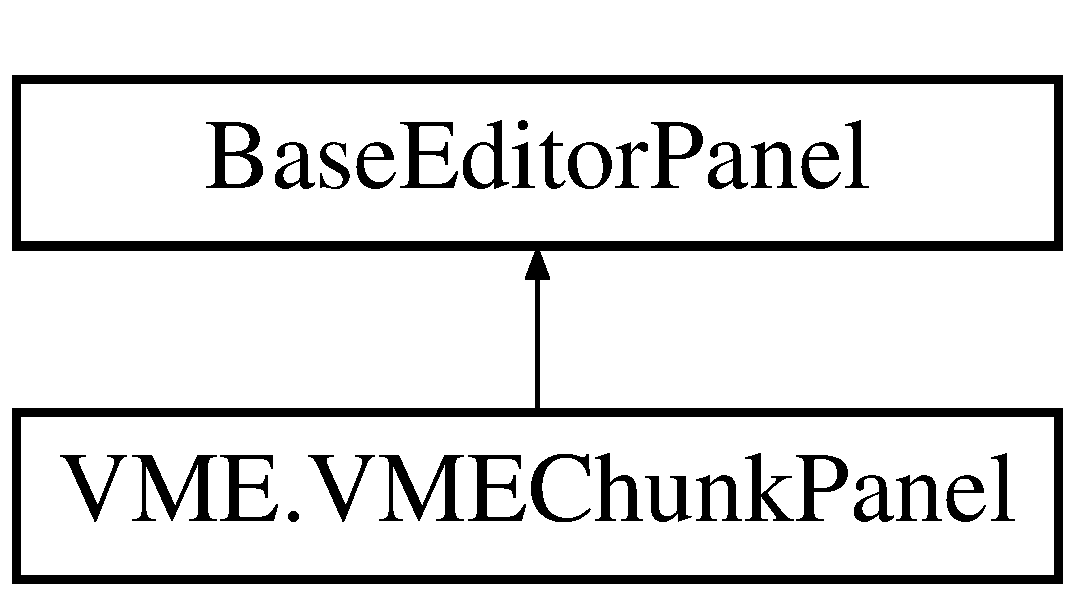
\includegraphics[height=2.000000cm]{class_v_m_e_1_1_v_m_e_chunk_panel}
\end{center}
\end{figure}
\subsection*{Public Member Functions}
\begin{DoxyCompactItemize}
\item 
\hyperlink{class_v_m_e_1_1_v_m_e_chunk_panel_afccc00c06110bf4a94a087d880ecec0c}{V\+M\+E\+Chunk\+Panel} (Editor\+Window \+\_\+window, Key\+Code \+\_\+toggle\+Key)
\begin{DoxyCompactList}\small\item\em Constructor. \end{DoxyCompactList}\item 
override void \hyperlink{class_v_m_e_1_1_v_m_e_chunk_panel_a61ffdb0c341b6571f8193a2c4caefb0e}{On\+Opened} ()
\begin{DoxyCompactList}\small\item\em Called when the panel is opened. \end{DoxyCompactList}\item 
override void \hyperlink{class_v_m_e_1_1_v_m_e_chunk_panel_a40223de4b7a04a2dc23a65fc57bfa387}{Draw\+Content} ()
\begin{DoxyCompactList}\small\item\em Draws the content of the panel. \end{DoxyCompactList}\item 
void \hyperlink{class_v_m_e_1_1_v_m_e_chunk_panel_a04dfe486fbbd8f3e3b9dff22d314ae0f}{Set\+Voxel\+Map} (\hyperlink{class_voxel_map}{Voxel\+Map} \+\_\+map)
\begin{DoxyCompactList}\small\item\em Changes the voxel map reference. \end{DoxyCompactList}\end{DoxyCompactItemize}
\subsection*{Additional Inherited Members}


\subsection{Detailed Description}
Panel used for the Chunks in the \hyperlink{namespace_v_m_e}{V\+ME} Editor. 



\subsection{Constructor \& Destructor Documentation}
\index{V\+M\+E\+::\+V\+M\+E\+Chunk\+Panel@{V\+M\+E\+::\+V\+M\+E\+Chunk\+Panel}!V\+M\+E\+Chunk\+Panel@{V\+M\+E\+Chunk\+Panel}}
\index{V\+M\+E\+Chunk\+Panel@{V\+M\+E\+Chunk\+Panel}!V\+M\+E\+::\+V\+M\+E\+Chunk\+Panel@{V\+M\+E\+::\+V\+M\+E\+Chunk\+Panel}}
\subsubsection[{\texorpdfstring{V\+M\+E\+Chunk\+Panel(\+Editor\+Window \+\_\+window, Key\+Code \+\_\+toggle\+Key)}{VMEChunkPanel(EditorWindow _window, KeyCode _toggleKey)}}]{\setlength{\rightskip}{0pt plus 5cm}V\+M\+E.\+V\+M\+E\+Chunk\+Panel.\+V\+M\+E\+Chunk\+Panel (
\begin{DoxyParamCaption}
\item[{Editor\+Window}]{\+\_\+window, }
\item[{Key\+Code}]{\+\_\+toggle\+Key}
\end{DoxyParamCaption}
)}\hypertarget{class_v_m_e_1_1_v_m_e_chunk_panel_afccc00c06110bf4a94a087d880ecec0c}{}\label{class_v_m_e_1_1_v_m_e_chunk_panel_afccc00c06110bf4a94a087d880ecec0c}


Constructor. 



\subsection{Member Function Documentation}
\index{V\+M\+E\+::\+V\+M\+E\+Chunk\+Panel@{V\+M\+E\+::\+V\+M\+E\+Chunk\+Panel}!Draw\+Content@{Draw\+Content}}
\index{Draw\+Content@{Draw\+Content}!V\+M\+E\+::\+V\+M\+E\+Chunk\+Panel@{V\+M\+E\+::\+V\+M\+E\+Chunk\+Panel}}
\subsubsection[{\texorpdfstring{Draw\+Content()}{DrawContent()}}]{\setlength{\rightskip}{0pt plus 5cm}override void V\+M\+E.\+V\+M\+E\+Chunk\+Panel.\+Draw\+Content (
\begin{DoxyParamCaption}
{}
\end{DoxyParamCaption}
)\hspace{0.3cm}{\ttfamily [virtual]}}\hypertarget{class_v_m_e_1_1_v_m_e_chunk_panel_a40223de4b7a04a2dc23a65fc57bfa387}{}\label{class_v_m_e_1_1_v_m_e_chunk_panel_a40223de4b7a04a2dc23a65fc57bfa387}


Draws the content of the panel. 



Reimplemented from \hyperlink{class_base_editor_panel_a96ea35bdda7a8e955baa1fd21635bffa}{Base\+Editor\+Panel}.

\index{V\+M\+E\+::\+V\+M\+E\+Chunk\+Panel@{V\+M\+E\+::\+V\+M\+E\+Chunk\+Panel}!On\+Opened@{On\+Opened}}
\index{On\+Opened@{On\+Opened}!V\+M\+E\+::\+V\+M\+E\+Chunk\+Panel@{V\+M\+E\+::\+V\+M\+E\+Chunk\+Panel}}
\subsubsection[{\texorpdfstring{On\+Opened()}{OnOpened()}}]{\setlength{\rightskip}{0pt plus 5cm}override void V\+M\+E.\+V\+M\+E\+Chunk\+Panel.\+On\+Opened (
\begin{DoxyParamCaption}
{}
\end{DoxyParamCaption}
)\hspace{0.3cm}{\ttfamily [virtual]}}\hypertarget{class_v_m_e_1_1_v_m_e_chunk_panel_a61ffdb0c341b6571f8193a2c4caefb0e}{}\label{class_v_m_e_1_1_v_m_e_chunk_panel_a61ffdb0c341b6571f8193a2c4caefb0e}


Called when the panel is opened. 



Reimplemented from \hyperlink{class_base_editor_panel_a3a8ccb88e5e34920880e9000a48fb862}{Base\+Editor\+Panel}.

\index{V\+M\+E\+::\+V\+M\+E\+Chunk\+Panel@{V\+M\+E\+::\+V\+M\+E\+Chunk\+Panel}!Set\+Voxel\+Map@{Set\+Voxel\+Map}}
\index{Set\+Voxel\+Map@{Set\+Voxel\+Map}!V\+M\+E\+::\+V\+M\+E\+Chunk\+Panel@{V\+M\+E\+::\+V\+M\+E\+Chunk\+Panel}}
\subsubsection[{\texorpdfstring{Set\+Voxel\+Map(\+Voxel\+Map \+\_\+map)}{SetVoxelMap(VoxelMap _map)}}]{\setlength{\rightskip}{0pt plus 5cm}void V\+M\+E.\+V\+M\+E\+Chunk\+Panel.\+Set\+Voxel\+Map (
\begin{DoxyParamCaption}
\item[{{\bf Voxel\+Map}}]{\+\_\+map}
\end{DoxyParamCaption}
)}\hypertarget{class_v_m_e_1_1_v_m_e_chunk_panel_a04dfe486fbbd8f3e3b9dff22d314ae0f}{}\label{class_v_m_e_1_1_v_m_e_chunk_panel_a04dfe486fbbd8f3e3b9dff22d314ae0f}


Changes the voxel map reference. 


\begin{DoxyParams}{Parameters}
{\em \+\_\+map} & the new reference.\\
\hline
\end{DoxyParams}


The documentation for this class was generated from the following file\+:\begin{DoxyCompactItemize}
\item 
C\+:/\+Users/\+Kevin Breurken/\+Documents/\+Projects/\+V\+M\+E/\+Assets/\+V\+M\+E/\+Editor/\+Voxel\+Map\+Editor/\+Panels/\+Editor/V\+M\+E\+Chunk\+Panel.\+cs\end{DoxyCompactItemize}

\hypertarget{class_v_m_e_1_1_v_m_e_edit_controls}{}\section{V\+M\+E.\+V\+M\+E\+Edit\+Controls Class Reference}
\label{class_v_m_e_1_1_v_m_e_edit_controls}\index{V\+M\+E.\+V\+M\+E\+Edit\+Controls@{V\+M\+E.\+V\+M\+E\+Edit\+Controls}}


Handles all related actions of editing a tile. actions like\+:  


\subsection*{Public Member Functions}
\begin{DoxyCompactItemize}
\item 
{\bfseries V\+M\+E\+Edit\+Controls} (\hyperlink{class_v_m_e_1_1_v_m_e_voxel_swatch_panel}{V\+M\+E\+Voxel\+Swatch\+Panel} \+\_\+voxelswatchpanel)\hypertarget{class_v_m_e_1_1_v_m_e_edit_controls_a216eee214415c409bceab92e31ea1d41}{}\label{class_v_m_e_1_1_v_m_e_edit_controls_a216eee214415c409bceab92e31ea1d41}

\item 
void \hyperlink{class_v_m_e_1_1_v_m_e_edit_controls_a07184e3c3b3dfc1adaac6379ce63bbfc}{Input} (Scene\+View view)
\begin{DoxyCompactList}\small\item\em Handles input for the editor. \end{DoxyCompactList}\end{DoxyCompactItemize}


\subsection{Detailed Description}
Handles all related actions of editing a tile. actions like\+: 

\mbox{[}edit tile to selection in Tile\+Swatch. (single or multiple selection) \mbox{]} \mbox{[}Change style of hovered tile\mbox{]} \mbox{[}Rotate hovered tile\mbox{]} 

\subsection{Member Function Documentation}
\index{V\+M\+E\+::\+V\+M\+E\+Edit\+Controls@{V\+M\+E\+::\+V\+M\+E\+Edit\+Controls}!Input@{Input}}
\index{Input@{Input}!V\+M\+E\+::\+V\+M\+E\+Edit\+Controls@{V\+M\+E\+::\+V\+M\+E\+Edit\+Controls}}
\subsubsection[{\texorpdfstring{Input(\+Scene\+View view)}{Input(SceneView view)}}]{\setlength{\rightskip}{0pt plus 5cm}void V\+M\+E.\+V\+M\+E\+Edit\+Controls.\+Input (
\begin{DoxyParamCaption}
\item[{Scene\+View}]{view}
\end{DoxyParamCaption}
)}\hypertarget{class_v_m_e_1_1_v_m_e_edit_controls_a07184e3c3b3dfc1adaac6379ce63bbfc}{}\label{class_v_m_e_1_1_v_m_e_edit_controls_a07184e3c3b3dfc1adaac6379ce63bbfc}


Handles input for the editor. 



The documentation for this class was generated from the following file\+:\begin{DoxyCompactItemize}
\item 
C\+:/\+Users/\+Kevin Breurken/\+Documents/\+Projects/\+V\+M\+E/\+Assets/\+V\+M\+E/\+Editor/\+Voxel\+Map\+Editor/\+Controls/V\+M\+E\+Edit\+Controls.\+cs\end{DoxyCompactItemize}

\hypertarget{class_v_m_e_1_1_v_m_e_file_manager_panel}{}\section{V\+M\+E.\+V\+M\+E\+File\+Manager\+Panel Class Reference}
\label{class_v_m_e_1_1_v_m_e_file_manager_panel}\index{V\+M\+E.\+V\+M\+E\+File\+Manager\+Panel@{V\+M\+E.\+V\+M\+E\+File\+Manager\+Panel}}
Inheritance diagram for V\+M\+E.\+V\+M\+E\+File\+Manager\+Panel\+:\begin{figure}[H]
\begin{center}
\leavevmode
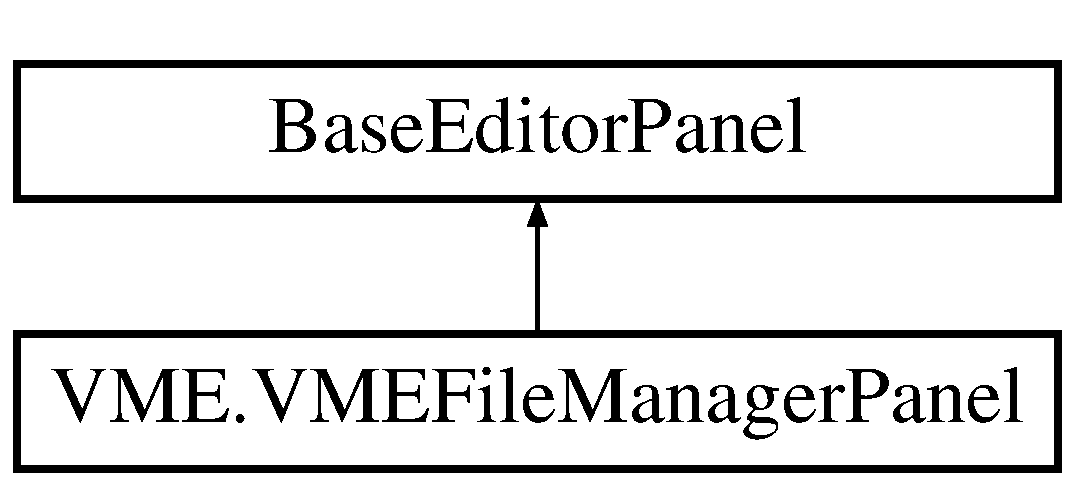
\includegraphics[height=2.000000cm]{class_v_m_e_1_1_v_m_e_file_manager_panel}
\end{center}
\end{figure}
\subsection*{Public Member Functions}
\begin{DoxyCompactItemize}
\item 
delegate void {\bfseries Voxel\+Map\+Action} (\hyperlink{class_voxel_map}{Voxel\+Map} \+\_\+map)\hypertarget{class_v_m_e_1_1_v_m_e_file_manager_panel_ab7337fc7b9361e273e2b708c11f04993}{}\label{class_v_m_e_1_1_v_m_e_file_manager_panel_ab7337fc7b9361e273e2b708c11f04993}

\item 
delegate void {\bfseries Voxel\+Swatch\+Action} (\hyperlink{class_voxel_swatch}{Voxel\+Swatch} \+\_\+swatch)\hypertarget{class_v_m_e_1_1_v_m_e_file_manager_panel_a01f2f73954d5080ff98c87e328495014}{}\label{class_v_m_e_1_1_v_m_e_file_manager_panel_a01f2f73954d5080ff98c87e328495014}

\item 
{\bfseries V\+M\+E\+File\+Manager\+Panel} (Editor\+Window \+\_\+window, Key\+Code \+\_\+toggle\+Key)\hypertarget{class_v_m_e_1_1_v_m_e_file_manager_panel_ad294f448fa6fb637dd8512727326f8d8}{}\label{class_v_m_e_1_1_v_m_e_file_manager_panel_ad294f448fa6fb637dd8512727326f8d8}

\item 
override void \hyperlink{class_v_m_e_1_1_v_m_e_file_manager_panel_a328194babcf088ee2e1a4ab89deeb916}{Draw\+Content} ()
\begin{DoxyCompactList}\small\item\em Draws the content of the panel. \end{DoxyCompactList}\item 
override void \hyperlink{class_v_m_e_1_1_v_m_e_file_manager_panel_ac39bb43df82776379e2f31c67b0ced93}{Input} (Scene\+View scene\+View)
\begin{DoxyCompactList}\small\item\em Used for handling keyboard input. \end{DoxyCompactList}\end{DoxyCompactItemize}
\subsection*{Public Attributes}
\begin{DoxyCompactItemize}
\item 
\hyperlink{class_voxel_map}{Voxel\+Map} {\bfseries voxel\+Map}\hypertarget{class_v_m_e_1_1_v_m_e_file_manager_panel_a4efcef4b19255ac2cd7c2a0d953560e7}{}\label{class_v_m_e_1_1_v_m_e_file_manager_panel_a4efcef4b19255ac2cd7c2a0d953560e7}

\item 
\hyperlink{class_voxel_swatch}{Voxel\+Swatch} {\bfseries voxel\+Swatch}\hypertarget{class_v_m_e_1_1_v_m_e_file_manager_panel_ae2575b94858df4f8e69552a98b1cc800}{}\label{class_v_m_e_1_1_v_m_e_file_manager_panel_ae2575b94858df4f8e69552a98b1cc800}

\end{DoxyCompactItemize}
\subsection*{Events}
\begin{DoxyCompactItemize}
\item 
Voxel\+Map\+Action {\bfseries On\+Voxel\+Map\+Changed\+Event}\hypertarget{class_v_m_e_1_1_v_m_e_file_manager_panel_a65600f51f02d0c0e13aed681620e436e}{}\label{class_v_m_e_1_1_v_m_e_file_manager_panel_a65600f51f02d0c0e13aed681620e436e}

\item 
Voxel\+Swatch\+Action {\bfseries On\+Voxel\+Swatch\+Changed\+Event}\hypertarget{class_v_m_e_1_1_v_m_e_file_manager_panel_ab4818edbfbd3c426eb10769e43ea5dca}{}\label{class_v_m_e_1_1_v_m_e_file_manager_panel_ab4818edbfbd3c426eb10769e43ea5dca}

\end{DoxyCompactItemize}


\subsection{Member Function Documentation}
\index{V\+M\+E\+::\+V\+M\+E\+File\+Manager\+Panel@{V\+M\+E\+::\+V\+M\+E\+File\+Manager\+Panel}!Draw\+Content@{Draw\+Content}}
\index{Draw\+Content@{Draw\+Content}!V\+M\+E\+::\+V\+M\+E\+File\+Manager\+Panel@{V\+M\+E\+::\+V\+M\+E\+File\+Manager\+Panel}}
\subsubsection[{\texorpdfstring{Draw\+Content()}{DrawContent()}}]{\setlength{\rightskip}{0pt plus 5cm}override void V\+M\+E.\+V\+M\+E\+File\+Manager\+Panel.\+Draw\+Content (
\begin{DoxyParamCaption}
{}
\end{DoxyParamCaption}
)\hspace{0.3cm}{\ttfamily [virtual]}}\hypertarget{class_v_m_e_1_1_v_m_e_file_manager_panel_a328194babcf088ee2e1a4ab89deeb916}{}\label{class_v_m_e_1_1_v_m_e_file_manager_panel_a328194babcf088ee2e1a4ab89deeb916}


Draws the content of the panel. 



Reimplemented from \hyperlink{class_base_editor_panel_a96ea35bdda7a8e955baa1fd21635bffa}{Base\+Editor\+Panel}.

\index{V\+M\+E\+::\+V\+M\+E\+File\+Manager\+Panel@{V\+M\+E\+::\+V\+M\+E\+File\+Manager\+Panel}!Input@{Input}}
\index{Input@{Input}!V\+M\+E\+::\+V\+M\+E\+File\+Manager\+Panel@{V\+M\+E\+::\+V\+M\+E\+File\+Manager\+Panel}}
\subsubsection[{\texorpdfstring{Input(\+Scene\+View scene\+View)}{Input(SceneView sceneView)}}]{\setlength{\rightskip}{0pt plus 5cm}override void V\+M\+E.\+V\+M\+E\+File\+Manager\+Panel.\+Input (
\begin{DoxyParamCaption}
\item[{Scene\+View}]{\+\_\+scene\+View}
\end{DoxyParamCaption}
)\hspace{0.3cm}{\ttfamily [virtual]}}\hypertarget{class_v_m_e_1_1_v_m_e_file_manager_panel_ac39bb43df82776379e2f31c67b0ced93}{}\label{class_v_m_e_1_1_v_m_e_file_manager_panel_ac39bb43df82776379e2f31c67b0ced93}


Used for handling keyboard input. 



Reimplemented from \hyperlink{class_base_editor_panel_a9bd01437be0e246418dc89209ef2125b}{Base\+Editor\+Panel}.



The documentation for this class was generated from the following file\+:\begin{DoxyCompactItemize}
\item 
C\+:/\+Users/\+Kevin Breurken/\+Documents/\+Projects/\+V\+M\+E/\+Assets/\+V\+M\+E/\+Editor/\+Voxel\+Map\+Editor/\+Panels/\+Editor/V\+M\+E\+File\+Manager\+Panel.\+cs\end{DoxyCompactItemize}

\hypertarget{class_v_m_e_1_1_v_m_e_global}{}\section{V\+M\+E.\+V\+M\+E\+Global Class Reference}
\label{class_v_m_e_1_1_v_m_e_global}\index{V\+M\+E.\+V\+M\+E\+Global@{V\+M\+E.\+V\+M\+E\+Global}}


Global functions used on multiple locations thereby easier to reference as a global function.  


\subsection*{Static Public Member Functions}
\begin{DoxyCompactItemize}
\item 
static Game\+Object \hyperlink{class_v_m_e_1_1_v_m_e_global_a671e5f258b3eb4bcadf664c167c3e79f}{Get\+Tile\+At\+Mouse\+Position} ()
\begin{DoxyCompactList}\small\item\em Returns the Game object on mouse position. \end{DoxyCompactList}\item 
static Vector3 \hyperlink{class_v_m_e_1_1_v_m_e_global_a69d7a0fa793e299c8abcd21f2cdfe4f5}{Get\+Position\+Next\+To\+Hovered\+Tile} ()
\begin{DoxyCompactList}\small\item\em Returns the position next to the side you pressed on. \end{DoxyCompactList}\end{DoxyCompactItemize}
\subsection*{Properties}
\begin{DoxyCompactItemize}
\item 
static bool \hyperlink{class_v_m_e_1_1_v_m_e_global_ae53c2b25ceae18d5585ced3817c65e20}{Hidden}\hspace{0.3cm}{\ttfamily  \mbox{[}get, set\mbox{]}}
\begin{DoxyCompactList}\small\item\em Hides the default transform controls. \end{DoxyCompactList}\end{DoxyCompactItemize}


\subsection{Detailed Description}
Global functions used on multiple locations thereby easier to reference as a global function. 



\subsection{Member Function Documentation}
\index{V\+M\+E\+::\+V\+M\+E\+Global@{V\+M\+E\+::\+V\+M\+E\+Global}!Get\+Position\+Next\+To\+Hovered\+Tile@{Get\+Position\+Next\+To\+Hovered\+Tile}}
\index{Get\+Position\+Next\+To\+Hovered\+Tile@{Get\+Position\+Next\+To\+Hovered\+Tile}!V\+M\+E\+::\+V\+M\+E\+Global@{V\+M\+E\+::\+V\+M\+E\+Global}}
\subsubsection[{\texorpdfstring{Get\+Position\+Next\+To\+Hovered\+Tile()}{GetPositionNextToHoveredTile()}}]{\setlength{\rightskip}{0pt plus 5cm}static Vector3 V\+M\+E.\+V\+M\+E\+Global.\+Get\+Position\+Next\+To\+Hovered\+Tile (
\begin{DoxyParamCaption}
{}
\end{DoxyParamCaption}
)\hspace{0.3cm}{\ttfamily [static]}}\hypertarget{class_v_m_e_1_1_v_m_e_global_a69d7a0fa793e299c8abcd21f2cdfe4f5}{}\label{class_v_m_e_1_1_v_m_e_global_a69d7a0fa793e299c8abcd21f2cdfe4f5}


Returns the position next to the side you pressed on. 

\index{V\+M\+E\+::\+V\+M\+E\+Global@{V\+M\+E\+::\+V\+M\+E\+Global}!Get\+Tile\+At\+Mouse\+Position@{Get\+Tile\+At\+Mouse\+Position}}
\index{Get\+Tile\+At\+Mouse\+Position@{Get\+Tile\+At\+Mouse\+Position}!V\+M\+E\+::\+V\+M\+E\+Global@{V\+M\+E\+::\+V\+M\+E\+Global}}
\subsubsection[{\texorpdfstring{Get\+Tile\+At\+Mouse\+Position()}{GetTileAtMousePosition()}}]{\setlength{\rightskip}{0pt plus 5cm}static Game\+Object V\+M\+E.\+V\+M\+E\+Global.\+Get\+Tile\+At\+Mouse\+Position (
\begin{DoxyParamCaption}
{}
\end{DoxyParamCaption}
)\hspace{0.3cm}{\ttfamily [static]}}\hypertarget{class_v_m_e_1_1_v_m_e_global_a671e5f258b3eb4bcadf664c167c3e79f}{}\label{class_v_m_e_1_1_v_m_e_global_a671e5f258b3eb4bcadf664c167c3e79f}


Returns the Game object on mouse position. 



\subsection{Property Documentation}
\index{V\+M\+E\+::\+V\+M\+E\+Global@{V\+M\+E\+::\+V\+M\+E\+Global}!Hidden@{Hidden}}
\index{Hidden@{Hidden}!V\+M\+E\+::\+V\+M\+E\+Global@{V\+M\+E\+::\+V\+M\+E\+Global}}
\subsubsection[{\texorpdfstring{Hidden}{Hidden}}]{\setlength{\rightskip}{0pt plus 5cm}bool V\+M\+E.\+V\+M\+E\+Global.\+Hidden\hspace{0.3cm}{\ttfamily [static]}, {\ttfamily [get]}, {\ttfamily [set]}}\hypertarget{class_v_m_e_1_1_v_m_e_global_ae53c2b25ceae18d5585ced3817c65e20}{}\label{class_v_m_e_1_1_v_m_e_global_ae53c2b25ceae18d5585ced3817c65e20}


Hides the default transform controls. 



The documentation for this class was generated from the following file\+:\begin{DoxyCompactItemize}
\item 
C\+:/\+Users/\+Kevin Breurken/\+Documents/\+Projects/\+V\+M\+E/\+Assets/\+V\+M\+E/\+Editor/V\+M\+E\+Global.\+cs\end{DoxyCompactItemize}

\hypertarget{class_v_m_e_1_1_v_m_e_main_panel}{}\section{V\+M\+E.\+V\+M\+E\+Main\+Panel Class Reference}
\label{class_v_m_e_1_1_v_m_e_main_panel}\index{V\+M\+E.\+V\+M\+E\+Main\+Panel@{V\+M\+E.\+V\+M\+E\+Main\+Panel}}


Voxel Map Main Panel.  


Inheritance diagram for V\+M\+E.\+V\+M\+E\+Main\+Panel\+:\begin{figure}[H]
\begin{center}
\leavevmode
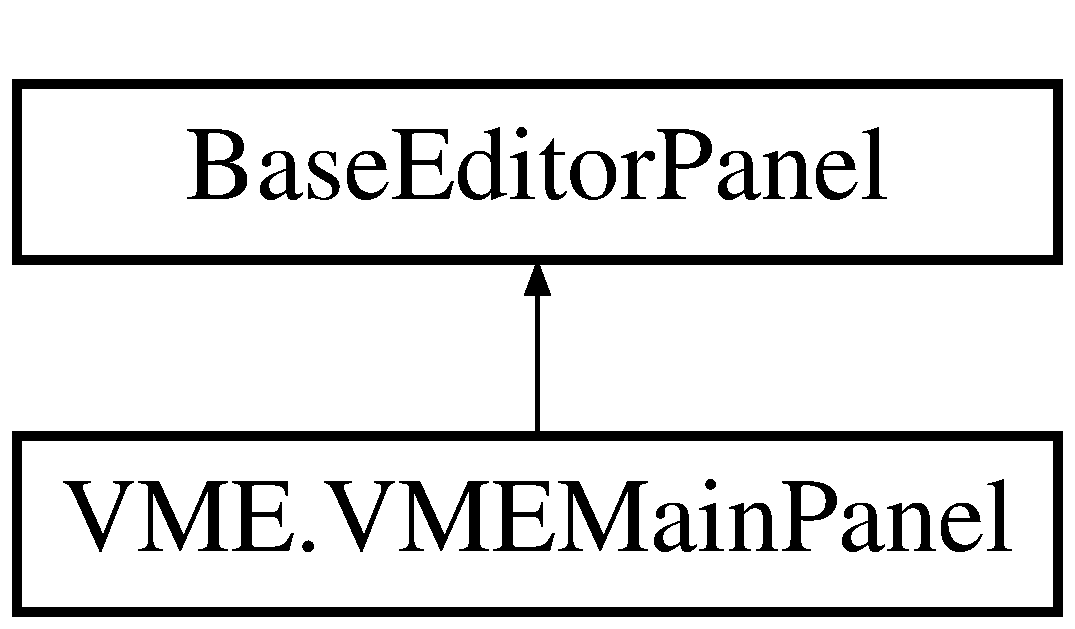
\includegraphics[height=2.000000cm]{class_v_m_e_1_1_v_m_e_main_panel}
\end{center}
\end{figure}
\subsection*{Public Member Functions}
\begin{DoxyCompactItemize}
\item 
{\bfseries V\+M\+E\+Main\+Panel} (Editor\+Window \+\_\+window, Key\+Code \+\_\+toggle\+Key)\hypertarget{class_v_m_e_1_1_v_m_e_main_panel_ab8d64c9d0dc0cdc5763d50cd9c4a40a8}{}\label{class_v_m_e_1_1_v_m_e_main_panel_ab8d64c9d0dc0cdc5763d50cd9c4a40a8}

\item 
override void \hyperlink{class_v_m_e_1_1_v_m_e_main_panel_a31c00f8725239c4e1758f32bb0d29cf9}{Draw\+Content} ()
\begin{DoxyCompactList}\small\item\em See \end{DoxyCompactList}\item 
override void \hyperlink{class_v_m_e_1_1_v_m_e_main_panel_a3ee8bf67ac932165d48986d3dbba1fb4}{Input} (Scene\+View scene\+View)
\begin{DoxyCompactList}\small\item\em See \hyperlink{class_base_editor_panel_a9bd01437be0e246418dc89209ef2125b}{Base\+Editor\+Panel.\+Input}. \end{DoxyCompactList}\end{DoxyCompactItemize}
\subsection*{Public Attributes}
\begin{DoxyCompactItemize}
\item 
\hyperlink{class_v_m_e_1_1_v_m_e_snap_panel}{V\+M\+E\+Snap\+Panel} \hyperlink{class_v_m_e_1_1_v_m_e_main_panel_a697a2743671d166cf175861e1194e840}{snap\+Panel} = new \hyperlink{class_v_m_e_1_1_v_m_e_snap_panel}{V\+M\+E\+Snap\+Panel}()
\begin{DoxyCompactList}\small\item\em Handles snap function and panel drawing. \end{DoxyCompactList}\end{DoxyCompactItemize}


\subsection{Detailed Description}
Voxel Map Main Panel. 

Used for handling and drawing Main related features. 

\subsection{Member Function Documentation}
\index{V\+M\+E\+::\+V\+M\+E\+Main\+Panel@{V\+M\+E\+::\+V\+M\+E\+Main\+Panel}!Draw\+Content@{Draw\+Content}}
\index{Draw\+Content@{Draw\+Content}!V\+M\+E\+::\+V\+M\+E\+Main\+Panel@{V\+M\+E\+::\+V\+M\+E\+Main\+Panel}}
\subsubsection[{\texorpdfstring{Draw\+Content()}{DrawContent()}}]{\setlength{\rightskip}{0pt plus 5cm}override void V\+M\+E.\+V\+M\+E\+Main\+Panel.\+Draw\+Content (
\begin{DoxyParamCaption}
{}
\end{DoxyParamCaption}
)\hspace{0.3cm}{\ttfamily [virtual]}}\hypertarget{class_v_m_e_1_1_v_m_e_main_panel_a31c00f8725239c4e1758f32bb0d29cf9}{}\label{class_v_m_e_1_1_v_m_e_main_panel_a31c00f8725239c4e1758f32bb0d29cf9}


See 



Reimplemented from \hyperlink{class_base_editor_panel_a96ea35bdda7a8e955baa1fd21635bffa}{Base\+Editor\+Panel}.

\index{V\+M\+E\+::\+V\+M\+E\+Main\+Panel@{V\+M\+E\+::\+V\+M\+E\+Main\+Panel}!Input@{Input}}
\index{Input@{Input}!V\+M\+E\+::\+V\+M\+E\+Main\+Panel@{V\+M\+E\+::\+V\+M\+E\+Main\+Panel}}
\subsubsection[{\texorpdfstring{Input(\+Scene\+View scene\+View)}{Input(SceneView sceneView)}}]{\setlength{\rightskip}{0pt plus 5cm}override void V\+M\+E.\+V\+M\+E\+Main\+Panel.\+Input (
\begin{DoxyParamCaption}
\item[{Scene\+View}]{scene\+View}
\end{DoxyParamCaption}
)\hspace{0.3cm}{\ttfamily [virtual]}}\hypertarget{class_v_m_e_1_1_v_m_e_main_panel_a3ee8bf67ac932165d48986d3dbba1fb4}{}\label{class_v_m_e_1_1_v_m_e_main_panel_a3ee8bf67ac932165d48986d3dbba1fb4}


See \hyperlink{class_base_editor_panel_a9bd01437be0e246418dc89209ef2125b}{Base\+Editor\+Panel.\+Input}. 



Reimplemented from \hyperlink{class_base_editor_panel_a9bd01437be0e246418dc89209ef2125b}{Base\+Editor\+Panel}.



\subsection{Member Data Documentation}
\index{V\+M\+E\+::\+V\+M\+E\+Main\+Panel@{V\+M\+E\+::\+V\+M\+E\+Main\+Panel}!snap\+Panel@{snap\+Panel}}
\index{snap\+Panel@{snap\+Panel}!V\+M\+E\+::\+V\+M\+E\+Main\+Panel@{V\+M\+E\+::\+V\+M\+E\+Main\+Panel}}
\subsubsection[{\texorpdfstring{snap\+Panel}{snapPanel}}]{\setlength{\rightskip}{0pt plus 5cm}{\bf V\+M\+E\+Snap\+Panel} V\+M\+E.\+V\+M\+E\+Main\+Panel.\+snap\+Panel = new {\bf V\+M\+E\+Snap\+Panel}()}\hypertarget{class_v_m_e_1_1_v_m_e_main_panel_a697a2743671d166cf175861e1194e840}{}\label{class_v_m_e_1_1_v_m_e_main_panel_a697a2743671d166cf175861e1194e840}


Handles snap function and panel drawing. 



The documentation for this class was generated from the following file\+:\begin{DoxyCompactItemize}
\item 
C\+:/\+Users/\+Kevin Breurken/\+Documents/\+Projects/\+V\+M\+E/\+Assets/\+V\+M\+E/\+Editor/\+Voxel\+Map\+Editor/\+Panels/\+Editor/V\+M\+E\+Main\+Panel.\+cs\end{DoxyCompactItemize}

\hypertarget{class_v_m_e_1_1_v_m_e_main_window}{}\section{V\+M\+E.\+V\+M\+E\+Main\+Window Class Reference}
\label{class_v_m_e_1_1_v_m_e_main_window}\index{V\+M\+E.\+V\+M\+E\+Main\+Window@{V\+M\+E.\+V\+M\+E\+Main\+Window}}


Voxel Map Main Editor window.  


Inheritance diagram for V\+M\+E.\+V\+M\+E\+Main\+Window\+:\begin{figure}[H]
\begin{center}
\leavevmode
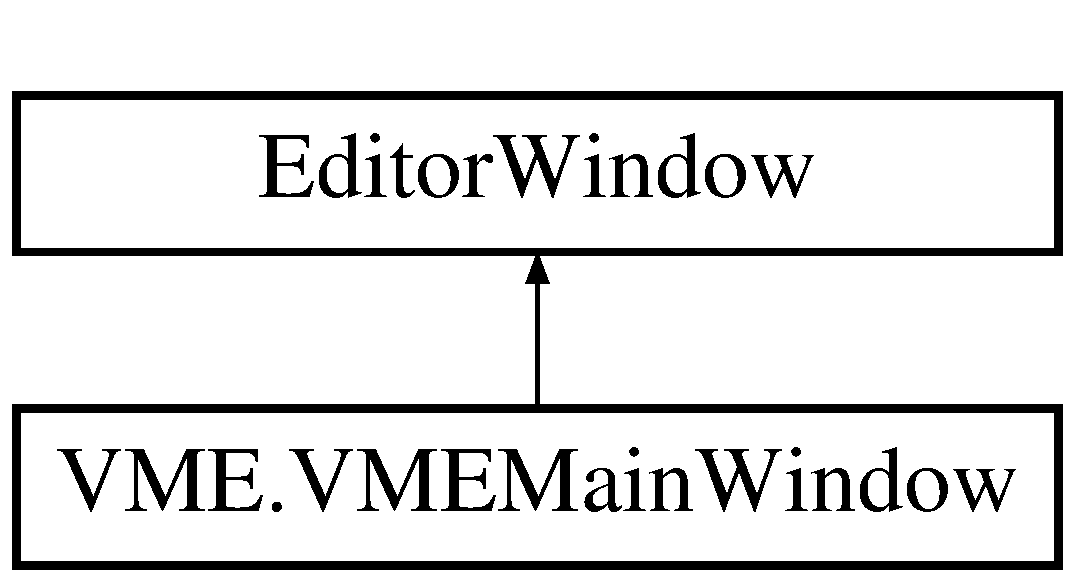
\includegraphics[height=2.000000cm]{class_v_m_e_1_1_v_m_e_main_window}
\end{center}
\end{figure}
\subsection*{Public Member Functions}
\begin{DoxyCompactItemize}
\item 
void \hyperlink{class_v_m_e_1_1_v_m_e_main_window_a066a36f1875066fb5ae745332222384c}{Update} ()
\begin{DoxyCompactList}\small\item\em For repainting the Window. \end{DoxyCompactList}\end{DoxyCompactItemize}
\subsection*{Public Attributes}
\begin{DoxyCompactItemize}
\item 
\hyperlink{class_v_m_e_tile_add_controls}{V\+M\+E\+Tile\+Add\+Controls} {\bfseries tile\+Add\+Controls}\hypertarget{class_v_m_e_1_1_v_m_e_main_window_a885b7fd4d66956f67e76766594280adf}{}\label{class_v_m_e_1_1_v_m_e_main_window_a885b7fd4d66956f67e76766594280adf}

\end{DoxyCompactItemize}
\subsection*{Static Public Attributes}
\begin{DoxyCompactItemize}
\item 
static \hyperlink{class_v_m_e_1_1_v_m_e_main_panel}{V\+M\+E\+Main\+Panel} {\bfseries main\+Panel}\hypertarget{class_v_m_e_1_1_v_m_e_main_window_a5a853a457bf6f7143c512b4805b39513}{}\label{class_v_m_e_1_1_v_m_e_main_window_a5a853a457bf6f7143c512b4805b39513}

\item 
static \hyperlink{class_v_m_e_1_1_v_m_e_selection_panel}{V\+M\+E\+Selection\+Panel} {\bfseries selection\+Panel}\hypertarget{class_v_m_e_1_1_v_m_e_main_window_a011d9d108ccf55ed948094be1f5841f7}{}\label{class_v_m_e_1_1_v_m_e_main_window_a011d9d108ccf55ed948094be1f5841f7}

\item 
static \hyperlink{class_v_m_e_1_1_v_m_e_voxel_swatch_panel}{V\+M\+E\+Voxel\+Swatch\+Panel} {\bfseries swatch\+Panel}\hypertarget{class_v_m_e_1_1_v_m_e_main_window_a1e940252cb466e5902e34a16daef3eaf}{}\label{class_v_m_e_1_1_v_m_e_main_window_a1e940252cb466e5902e34a16daef3eaf}

\item 
static \hyperlink{class_v_m_e_1_1_v_m_e_file_manager_panel}{V\+M\+E\+File\+Manager\+Panel} {\bfseries file\+Manager}\hypertarget{class_v_m_e_1_1_v_m_e_main_window_a68db00d53ad911e2d516c43a508b6d97}{}\label{class_v_m_e_1_1_v_m_e_main_window_a68db00d53ad911e2d516c43a508b6d97}

\item 
static \hyperlink{class_v_m_e_1_1_v_m_e_mode_panel}{V\+M\+E\+Mode\+Panel} {\bfseries mode\+Panel}\hypertarget{class_v_m_e_1_1_v_m_e_main_window_a5703dc44df6550b49e9f0f534828bddc}{}\label{class_v_m_e_1_1_v_m_e_main_window_a5703dc44df6550b49e9f0f534828bddc}

\item 
static \hyperlink{class_v_m_e_1_1_v_m_e_chunk_panel}{V\+M\+E\+Chunk\+Panel} {\bfseries chunk\+Panel}\hypertarget{class_v_m_e_1_1_v_m_e_main_window_aafe7502daf7d91d2dc40a1593ed782af}{}\label{class_v_m_e_1_1_v_m_e_main_window_aafe7502daf7d91d2dc40a1593ed782af}

\end{DoxyCompactItemize}
\subsection*{Properties}
\begin{DoxyCompactItemize}
\item 
static \hyperlink{class_v_m_e_1_1_v_m_e_main_window}{V\+M\+E\+Main\+Window} {\bfseries Instance}\hspace{0.3cm}{\ttfamily  \mbox{[}get\mbox{]}}\hypertarget{class_v_m_e_1_1_v_m_e_main_window_ae3d8c72e99a172c27ad5addfc810f903}{}\label{class_v_m_e_1_1_v_m_e_main_window_ae3d8c72e99a172c27ad5addfc810f903}

\end{DoxyCompactItemize}


\subsection{Detailed Description}
Voxel Map Main Editor window. 

Holds all the panels and other classes for the editor, Connects the functions used in panels ( ex. Editor Input / Editor Draw ) 

\subsection{Member Function Documentation}
\index{V\+M\+E\+::\+V\+M\+E\+Main\+Window@{V\+M\+E\+::\+V\+M\+E\+Main\+Window}!Update@{Update}}
\index{Update@{Update}!V\+M\+E\+::\+V\+M\+E\+Main\+Window@{V\+M\+E\+::\+V\+M\+E\+Main\+Window}}
\subsubsection[{\texorpdfstring{Update()}{Update()}}]{\setlength{\rightskip}{0pt plus 5cm}void V\+M\+E.\+V\+M\+E\+Main\+Window.\+Update (
\begin{DoxyParamCaption}
{}
\end{DoxyParamCaption}
)}\hypertarget{class_v_m_e_1_1_v_m_e_main_window_a066a36f1875066fb5ae745332222384c}{}\label{class_v_m_e_1_1_v_m_e_main_window_a066a36f1875066fb5ae745332222384c}


For repainting the Window. 



The documentation for this class was generated from the following file\+:\begin{DoxyCompactItemize}
\item 
C\+:/\+Users/\+Kevin Breurken/\+Documents/\+Projects/\+V\+M\+E/\+Assets/\+V\+M\+E/\+Editor/\+Voxel\+Map\+Editor/\+Windows/V\+M\+E\+Window.\+cs\end{DoxyCompactItemize}

\hypertarget{class_v_m_e_menu_item}{}\section{V\+M\+E\+Menu\+Item Class Reference}
\label{class_v_m_e_menu_item}\index{V\+M\+E\+Menu\+Item@{V\+M\+E\+Menu\+Item}}


Used for adding \hyperlink{namespace_v_m_e}{V\+ME} related Menu Items.  


Inheritance diagram for V\+M\+E\+Menu\+Item\+:\begin{figure}[H]
\begin{center}
\leavevmode
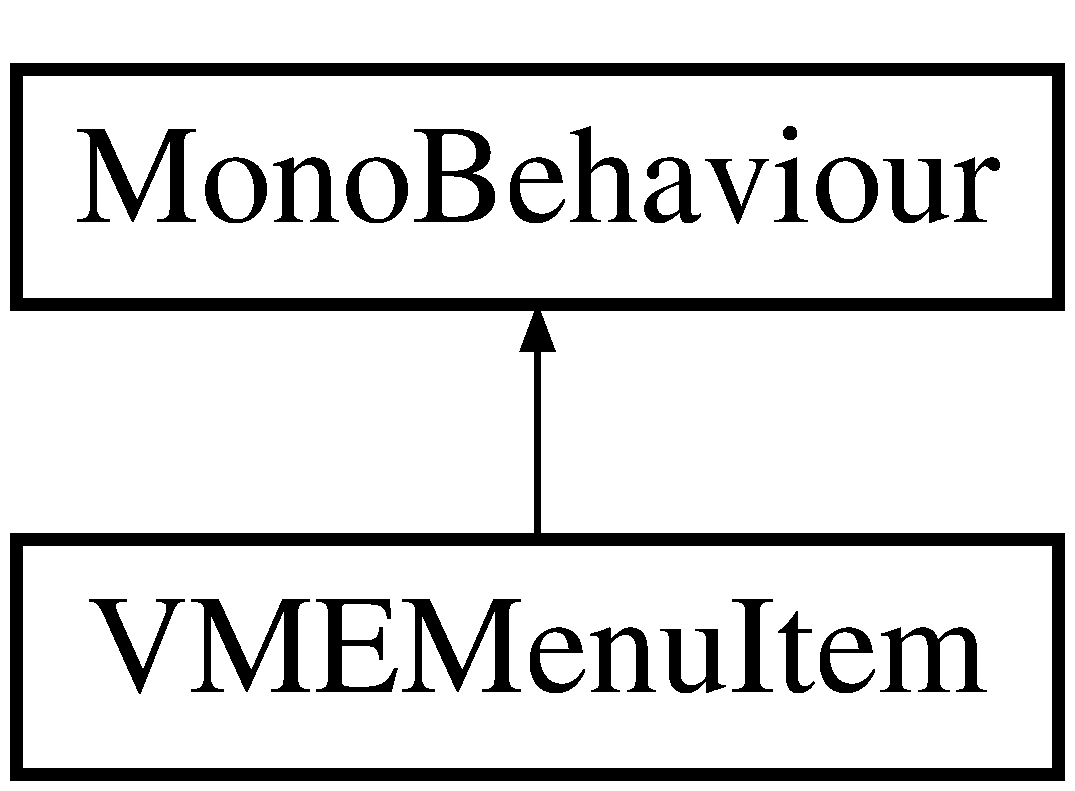
\includegraphics[height=2.000000cm]{class_v_m_e_menu_item}
\end{center}
\end{figure}


\subsection{Detailed Description}
Used for adding \hyperlink{namespace_v_m_e}{V\+ME} related Menu Items. 



The documentation for this class was generated from the following file\+:\begin{DoxyCompactItemize}
\item 
C\+:/\+Users/\+Kevin Breurken/\+Documents/\+Projects/\+V\+M\+E/\+Assets/\+V\+M\+E/\+Editor/\+Voxel\+Map\+Editor/V\+M\+E\+Menu\+Item.\+cs\end{DoxyCompactItemize}

\hypertarget{class_v_m_e_1_1_v_m_e_mode_panel}{}\section{V\+M\+E.\+V\+M\+E\+Mode\+Panel Class Reference}
\label{class_v_m_e_1_1_v_m_e_mode_panel}\index{V\+M\+E.\+V\+M\+E\+Mode\+Panel@{V\+M\+E.\+V\+M\+E\+Mode\+Panel}}
Inheritance diagram for V\+M\+E.\+V\+M\+E\+Mode\+Panel\+:\begin{figure}[H]
\begin{center}
\leavevmode
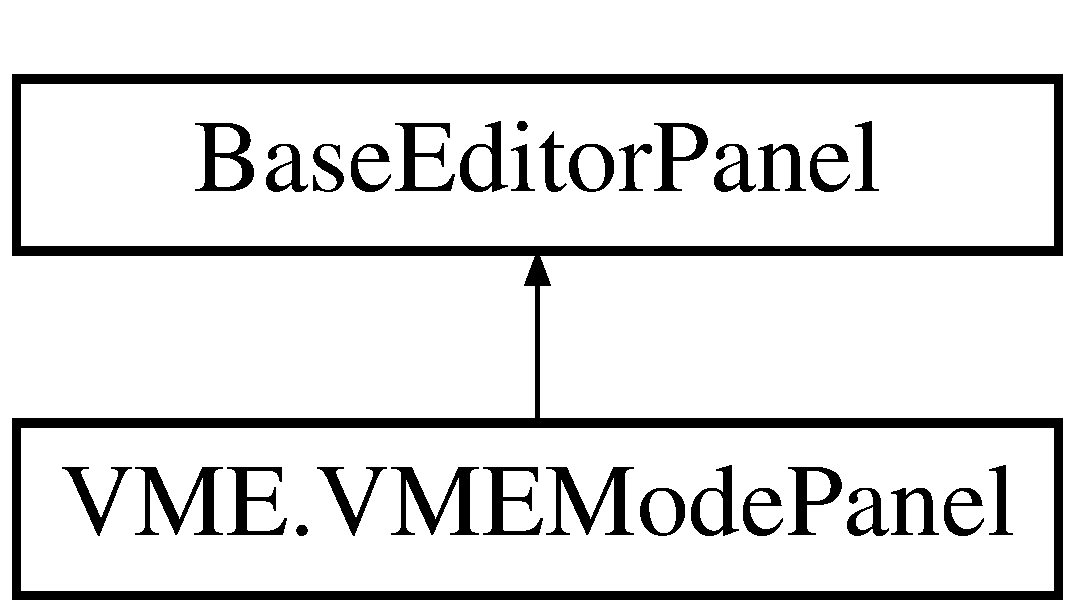
\includegraphics[height=2.000000cm]{class_v_m_e_1_1_v_m_e_mode_panel}
\end{center}
\end{figure}
\subsection*{Public Member Functions}
\begin{DoxyCompactItemize}
\item 
{\bfseries V\+M\+E\+Mode\+Panel} (Editor\+Window \+\_\+window, Key\+Code \+\_\+toggle\+Key, \hyperlink{class_v_m_e_1_1_v_m_e_voxel_swatch_panel}{V\+M\+E\+Voxel\+Swatch\+Panel} \+\_\+swatch\+Panel)\hypertarget{class_v_m_e_1_1_v_m_e_mode_panel_a6be58880200d43400636c18ff751c55d}{}\label{class_v_m_e_1_1_v_m_e_mode_panel_a6be58880200d43400636c18ff751c55d}

\item 
override void \hyperlink{class_v_m_e_1_1_v_m_e_mode_panel_ab60ed5d8ad208884843eb77a0633986d}{Draw\+Content} ()
\begin{DoxyCompactList}\small\item\em Draws the content of the panel. \end{DoxyCompactList}\item 
override void \hyperlink{class_v_m_e_1_1_v_m_e_mode_panel_adef41bb2208966390ef8557311fd576f}{Input} (Scene\+View scene\+View)
\begin{DoxyCompactList}\small\item\em Used for handling keyboard input. \end{DoxyCompactList}\item 
override void \hyperlink{class_v_m_e_1_1_v_m_e_mode_panel_a20fc99c3b9d0dc77b0b8bd72ed070177}{On\+Scene\+UI} (Scene\+View \+\_\+scene\+View)
\begin{DoxyCompactList}\small\item\em Used for drawing in the scene view. \end{DoxyCompactList}\end{DoxyCompactItemize}
\subsection*{Additional Inherited Members}


\subsection{Member Function Documentation}
\index{V\+M\+E\+::\+V\+M\+E\+Mode\+Panel@{V\+M\+E\+::\+V\+M\+E\+Mode\+Panel}!Draw\+Content@{Draw\+Content}}
\index{Draw\+Content@{Draw\+Content}!V\+M\+E\+::\+V\+M\+E\+Mode\+Panel@{V\+M\+E\+::\+V\+M\+E\+Mode\+Panel}}
\subsubsection[{\texorpdfstring{Draw\+Content()}{DrawContent()}}]{\setlength{\rightskip}{0pt plus 5cm}override void V\+M\+E.\+V\+M\+E\+Mode\+Panel.\+Draw\+Content (
\begin{DoxyParamCaption}
{}
\end{DoxyParamCaption}
)\hspace{0.3cm}{\ttfamily [virtual]}}\hypertarget{class_v_m_e_1_1_v_m_e_mode_panel_ab60ed5d8ad208884843eb77a0633986d}{}\label{class_v_m_e_1_1_v_m_e_mode_panel_ab60ed5d8ad208884843eb77a0633986d}


Draws the content of the panel. 



Reimplemented from \hyperlink{class_base_editor_panel_a96ea35bdda7a8e955baa1fd21635bffa}{Base\+Editor\+Panel}.

\index{V\+M\+E\+::\+V\+M\+E\+Mode\+Panel@{V\+M\+E\+::\+V\+M\+E\+Mode\+Panel}!Input@{Input}}
\index{Input@{Input}!V\+M\+E\+::\+V\+M\+E\+Mode\+Panel@{V\+M\+E\+::\+V\+M\+E\+Mode\+Panel}}
\subsubsection[{\texorpdfstring{Input(\+Scene\+View scene\+View)}{Input(SceneView sceneView)}}]{\setlength{\rightskip}{0pt plus 5cm}override void V\+M\+E.\+V\+M\+E\+Mode\+Panel.\+Input (
\begin{DoxyParamCaption}
\item[{Scene\+View}]{\+\_\+scene\+View}
\end{DoxyParamCaption}
)\hspace{0.3cm}{\ttfamily [virtual]}}\hypertarget{class_v_m_e_1_1_v_m_e_mode_panel_adef41bb2208966390ef8557311fd576f}{}\label{class_v_m_e_1_1_v_m_e_mode_panel_adef41bb2208966390ef8557311fd576f}


Used for handling keyboard input. 



Reimplemented from \hyperlink{class_base_editor_panel_a9bd01437be0e246418dc89209ef2125b}{Base\+Editor\+Panel}.

\index{V\+M\+E\+::\+V\+M\+E\+Mode\+Panel@{V\+M\+E\+::\+V\+M\+E\+Mode\+Panel}!On\+Scene\+UI@{On\+Scene\+UI}}
\index{On\+Scene\+UI@{On\+Scene\+UI}!V\+M\+E\+::\+V\+M\+E\+Mode\+Panel@{V\+M\+E\+::\+V\+M\+E\+Mode\+Panel}}
\subsubsection[{\texorpdfstring{On\+Scene\+U\+I(\+Scene\+View \+\_\+scene\+View)}{OnSceneUI(SceneView _sceneView)}}]{\setlength{\rightskip}{0pt plus 5cm}override void V\+M\+E.\+V\+M\+E\+Mode\+Panel.\+On\+Scene\+UI (
\begin{DoxyParamCaption}
\item[{Scene\+View}]{\+\_\+scene\+View}
\end{DoxyParamCaption}
)\hspace{0.3cm}{\ttfamily [virtual]}}\hypertarget{class_v_m_e_1_1_v_m_e_mode_panel_a20fc99c3b9d0dc77b0b8bd72ed070177}{}\label{class_v_m_e_1_1_v_m_e_mode_panel_a20fc99c3b9d0dc77b0b8bd72ed070177}


Used for drawing in the scene view. 



Reimplemented from \hyperlink{class_base_editor_panel_a720cd4b21ce5c74b52ba310d9978e6e3}{Base\+Editor\+Panel}.



The documentation for this class was generated from the following file\+:\begin{DoxyCompactItemize}
\item 
C\+:/\+Users/\+Kevin Breurken/\+Documents/\+Projects/\+V\+M\+E/\+Assets/\+V\+M\+E/\+Editor/\+Voxel\+Map\+Editor/\+Panels/\+Editor/V\+M\+E\+Mode\+Panel.\+cs\end{DoxyCompactItemize}

\hypertarget{class_v_m_e_1_1_v_m_e_paint_controls}{}\section{V\+M\+E.\+V\+M\+E\+Paint\+Controls Class Reference}
\label{class_v_m_e_1_1_v_m_e_paint_controls}\index{V\+M\+E.\+V\+M\+E\+Paint\+Controls@{V\+M\+E.\+V\+M\+E\+Paint\+Controls}}


Controls for painting a tile.  


\subsection*{Public Member Functions}
\begin{DoxyCompactItemize}
\item 
{\bfseries V\+M\+E\+Paint\+Controls} (\hyperlink{class_v_m_e_1_1_v_m_e_voxel_swatch_panel}{V\+M\+E\+Voxel\+Swatch\+Panel} \+\_\+voxelswatchpanel)\hypertarget{class_v_m_e_1_1_v_m_e_paint_controls_adf1c8518e7482f8c9dc60c3689522fcf}{}\label{class_v_m_e_1_1_v_m_e_paint_controls_adf1c8518e7482f8c9dc60c3689522fcf}

\item 
void \hyperlink{class_v_m_e_1_1_v_m_e_paint_controls_a2bca3f29d49888d2f347372cccca6c3e}{Input} (Scene\+View view)
\begin{DoxyCompactList}\small\item\em Handles input for the editor. \end{DoxyCompactList}\item 
void {\bfseries Paint\+At\+Hover\+Position} ()\hypertarget{class_v_m_e_1_1_v_m_e_paint_controls_ad6b6ad3272b64d521e87022ab2d8298f}{}\label{class_v_m_e_1_1_v_m_e_paint_controls_ad6b6ad3272b64d521e87022ab2d8298f}

\item 
void {\bfseries Paint\+All\+Inside\+Selection} ()\hypertarget{class_v_m_e_1_1_v_m_e_paint_controls_a4e93f94dc7530adb6864d47f99677507}{}\label{class_v_m_e_1_1_v_m_e_paint_controls_a4e93f94dc7530adb6864d47f99677507}

\end{DoxyCompactItemize}


\subsection{Detailed Description}
Controls for painting a tile. 



\subsection{Member Function Documentation}
\index{V\+M\+E\+::\+V\+M\+E\+Paint\+Controls@{V\+M\+E\+::\+V\+M\+E\+Paint\+Controls}!Input@{Input}}
\index{Input@{Input}!V\+M\+E\+::\+V\+M\+E\+Paint\+Controls@{V\+M\+E\+::\+V\+M\+E\+Paint\+Controls}}
\subsubsection[{\texorpdfstring{Input(\+Scene\+View view)}{Input(SceneView view)}}]{\setlength{\rightskip}{0pt plus 5cm}void V\+M\+E.\+V\+M\+E\+Paint\+Controls.\+Input (
\begin{DoxyParamCaption}
\item[{Scene\+View}]{view}
\end{DoxyParamCaption}
)}\hypertarget{class_v_m_e_1_1_v_m_e_paint_controls_a2bca3f29d49888d2f347372cccca6c3e}{}\label{class_v_m_e_1_1_v_m_e_paint_controls_a2bca3f29d49888d2f347372cccca6c3e}


Handles input for the editor. 



The documentation for this class was generated from the following file\+:\begin{DoxyCompactItemize}
\item 
C\+:/\+Users/\+Kevin Breurken/\+Documents/\+Projects/\+V\+M\+E/\+Assets/\+V\+M\+E/\+Editor/\+Voxel\+Map\+Editor/\+Controls/V\+M\+E\+Paint\+Controls.\+cs\end{DoxyCompactItemize}

\hypertarget{class_v_m_e_picker_controls}{}\section{V\+M\+E\+Picker\+Controls Class Reference}
\label{class_v_m_e_picker_controls}\index{V\+M\+E\+Picker\+Controls@{V\+M\+E\+Picker\+Controls}}
Inheritance diagram for V\+M\+E\+Picker\+Controls\+:\begin{figure}[H]
\begin{center}
\leavevmode
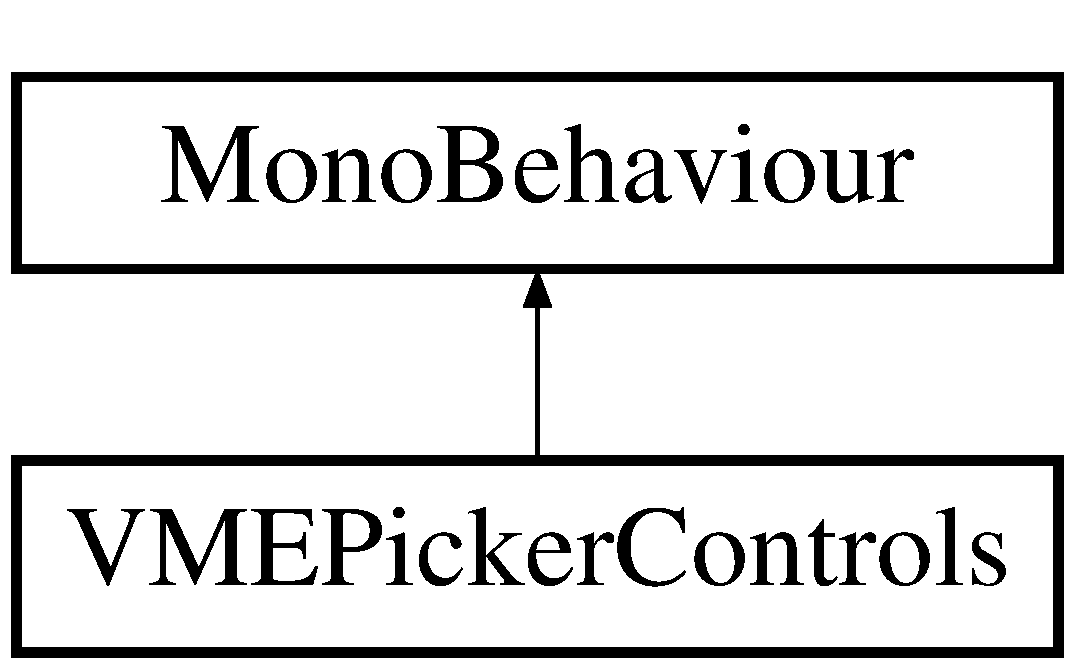
\includegraphics[height=2.000000cm]{class_v_m_e_picker_controls}
\end{center}
\end{figure}


The documentation for this class was generated from the following file\+:\begin{DoxyCompactItemize}
\item 
C\+:/\+Users/\+Kevin Breurken/\+Documents/\+Projects/\+V\+M\+E/\+Assets/\+V\+M\+E/\+Editor/\+Voxel\+Map\+Editor/\+Controls/V\+M\+E\+Picker\+Controls.\+cs\end{DoxyCompactItemize}

\hypertarget{class_v_m_e_1_1_v_m_e_selection_controls}{}\section{V\+M\+E.\+V\+M\+E\+Selection\+Controls Class Reference}
\label{class_v_m_e_1_1_v_m_e_selection_controls}\index{V\+M\+E.\+V\+M\+E\+Selection\+Controls@{V\+M\+E.\+V\+M\+E\+Selection\+Controls}}


Handles the controls for selecting tiles.  


\subsection*{Public Member Functions}
\begin{DoxyCompactItemize}
\item 
\hyperlink{class_v_m_e_1_1_v_m_e_selection_controls_a5013d2b1878c76245b7f939b24fdea41}{V\+M\+E\+Selection\+Controls} ()
\begin{DoxyCompactList}\small\item\em Constructor. \end{DoxyCompactList}\item 
void \hyperlink{class_v_m_e_1_1_v_m_e_selection_controls_a37bda8d1eb55a79327113feb01c1ff27}{Input} (Scene\+View view)
\begin{DoxyCompactList}\small\item\em Handles editor input. \end{DoxyCompactList}\end{DoxyCompactItemize}


\subsection{Detailed Description}
Handles the controls for selecting tiles. 



\subsection{Constructor \& Destructor Documentation}
\index{V\+M\+E\+::\+V\+M\+E\+Selection\+Controls@{V\+M\+E\+::\+V\+M\+E\+Selection\+Controls}!V\+M\+E\+Selection\+Controls@{V\+M\+E\+Selection\+Controls}}
\index{V\+M\+E\+Selection\+Controls@{V\+M\+E\+Selection\+Controls}!V\+M\+E\+::\+V\+M\+E\+Selection\+Controls@{V\+M\+E\+::\+V\+M\+E\+Selection\+Controls}}
\subsubsection[{\texorpdfstring{V\+M\+E\+Selection\+Controls()}{VMESelectionControls()}}]{\setlength{\rightskip}{0pt plus 5cm}V\+M\+E.\+V\+M\+E\+Selection\+Controls.\+V\+M\+E\+Selection\+Controls (
\begin{DoxyParamCaption}
{}
\end{DoxyParamCaption}
)}\hypertarget{class_v_m_e_1_1_v_m_e_selection_controls_a5013d2b1878c76245b7f939b24fdea41}{}\label{class_v_m_e_1_1_v_m_e_selection_controls_a5013d2b1878c76245b7f939b24fdea41}


Constructor. 



\subsection{Member Function Documentation}
\index{V\+M\+E\+::\+V\+M\+E\+Selection\+Controls@{V\+M\+E\+::\+V\+M\+E\+Selection\+Controls}!Input@{Input}}
\index{Input@{Input}!V\+M\+E\+::\+V\+M\+E\+Selection\+Controls@{V\+M\+E\+::\+V\+M\+E\+Selection\+Controls}}
\subsubsection[{\texorpdfstring{Input(\+Scene\+View view)}{Input(SceneView view)}}]{\setlength{\rightskip}{0pt plus 5cm}void V\+M\+E.\+V\+M\+E\+Selection\+Controls.\+Input (
\begin{DoxyParamCaption}
\item[{Scene\+View}]{view}
\end{DoxyParamCaption}
)}\hypertarget{class_v_m_e_1_1_v_m_e_selection_controls_a37bda8d1eb55a79327113feb01c1ff27}{}\label{class_v_m_e_1_1_v_m_e_selection_controls_a37bda8d1eb55a79327113feb01c1ff27}


Handles editor input. 



The documentation for this class was generated from the following file\+:\begin{DoxyCompactItemize}
\item 
C\+:/\+Users/\+Kevin Breurken/\+Documents/\+Projects/\+V\+M\+E/\+Assets/\+V\+M\+E/\+Editor/\+Voxel\+Map\+Editor/\+Controls/V\+M\+E\+Selection\+Controls.\+cs\end{DoxyCompactItemize}

\hypertarget{class_v_m_e_1_1_v_m_e_selection_panel}{}\section{V\+M\+E.\+V\+M\+E\+Selection\+Panel Class Reference}
\label{class_v_m_e_1_1_v_m_e_selection_panel}\index{V\+M\+E.\+V\+M\+E\+Selection\+Panel@{V\+M\+E.\+V\+M\+E\+Selection\+Panel}}


Shows info of current selection  


\subsection*{Public Member Functions}
\begin{DoxyCompactItemize}
\item 
void {\bfseries Draw} ()\hypertarget{class_v_m_e_1_1_v_m_e_selection_panel_ace194e8e28d5d546c24896bdc61386dc}{}\label{class_v_m_e_1_1_v_m_e_selection_panel_ace194e8e28d5d546c24896bdc61386dc}

\end{DoxyCompactItemize}


\subsection{Detailed Description}
Shows info of current selection 



The documentation for this class was generated from the following file\+:\begin{DoxyCompactItemize}
\item 
C\+:/\+Users/\+Kevin Breurken/\+Documents/\+Projects/\+V\+M\+E/\+Assets/\+V\+M\+E/\+Editor/\+Voxel\+Map\+Editor/\+Panels/V\+M\+E\+Selection\+Panel.\+cs\end{DoxyCompactItemize}

\hypertarget{class_v_m_e_1_1_settings_1_1_v_m_e_settings_key_panel}{}\section{V\+M\+E.\+Settings.\+V\+M\+E\+Settings\+Key\+Panel Class Reference}
\label{class_v_m_e_1_1_settings_1_1_v_m_e_settings_key_panel}\index{V\+M\+E.\+Settings.\+V\+M\+E\+Settings\+Key\+Panel@{V\+M\+E.\+Settings.\+V\+M\+E\+Settings\+Key\+Panel}}
Inheritance diagram for V\+M\+E.\+Settings.\+V\+M\+E\+Settings\+Key\+Panel\+:\begin{figure}[H]
\begin{center}
\leavevmode
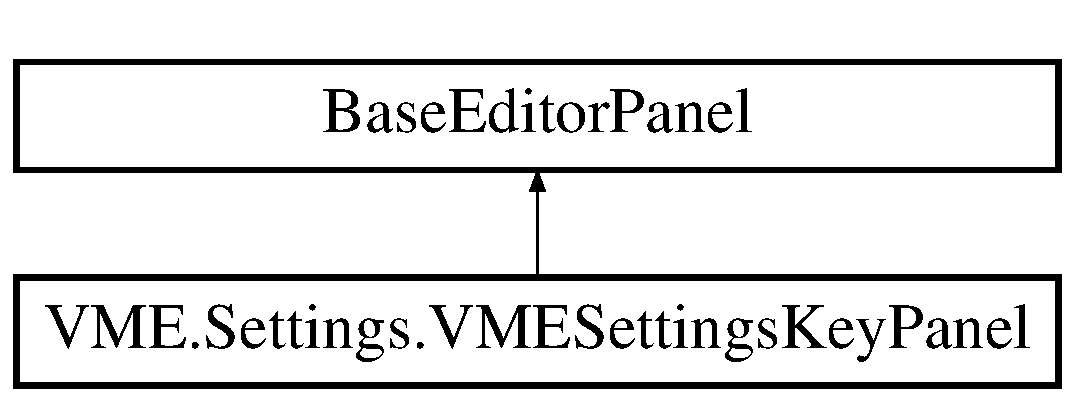
\includegraphics[height=2.000000cm]{class_v_m_e_1_1_settings_1_1_v_m_e_settings_key_panel}
\end{center}
\end{figure}
\subsection*{Public Member Functions}
\begin{DoxyCompactItemize}
\item 
{\bfseries V\+M\+E\+Settings\+Key\+Panel} (\hyperlink{class_v_m_e_settings_object}{V\+M\+E\+Settings\+Object} \+\_\+object)\hypertarget{class_v_m_e_1_1_settings_1_1_v_m_e_settings_key_panel_a28ab72df27950080ca08aa88af7f9b69}{}\label{class_v_m_e_1_1_settings_1_1_v_m_e_settings_key_panel_a28ab72df27950080ca08aa88af7f9b69}

\item 
override void \hyperlink{class_v_m_e_1_1_settings_1_1_v_m_e_settings_key_panel_a37a1629cea9d0dedcc887d52d54b036c}{Draw\+Content} ()
\begin{DoxyCompactList}\small\item\em Draws the content of the panel. \end{DoxyCompactList}\end{DoxyCompactItemize}
\subsection*{Additional Inherited Members}


\subsection{Member Function Documentation}
\index{V\+M\+E\+::\+Settings\+::\+V\+M\+E\+Settings\+Key\+Panel@{V\+M\+E\+::\+Settings\+::\+V\+M\+E\+Settings\+Key\+Panel}!Draw\+Content@{Draw\+Content}}
\index{Draw\+Content@{Draw\+Content}!V\+M\+E\+::\+Settings\+::\+V\+M\+E\+Settings\+Key\+Panel@{V\+M\+E\+::\+Settings\+::\+V\+M\+E\+Settings\+Key\+Panel}}
\subsubsection[{\texorpdfstring{Draw\+Content()}{DrawContent()}}]{\setlength{\rightskip}{0pt plus 5cm}override void V\+M\+E.\+Settings.\+V\+M\+E\+Settings\+Key\+Panel.\+Draw\+Content (
\begin{DoxyParamCaption}
{}
\end{DoxyParamCaption}
)\hspace{0.3cm}{\ttfamily [virtual]}}\hypertarget{class_v_m_e_1_1_settings_1_1_v_m_e_settings_key_panel_a37a1629cea9d0dedcc887d52d54b036c}{}\label{class_v_m_e_1_1_settings_1_1_v_m_e_settings_key_panel_a37a1629cea9d0dedcc887d52d54b036c}


Draws the content of the panel. 



Reimplemented from \hyperlink{class_base_editor_panel_a96ea35bdda7a8e955baa1fd21635bffa}{Base\+Editor\+Panel}.



The documentation for this class was generated from the following file\+:\begin{DoxyCompactItemize}
\item 
C\+:/\+Users/\+Kevin Breurken/\+Documents/\+Projects/\+V\+M\+E/\+Assets/\+V\+M\+E/\+Editor/\+Voxel\+Map\+Editor/\+Panels/\+Settings/V\+M\+E\+Settings\+Key\+Panel.\+cs\end{DoxyCompactItemize}

\hypertarget{class_v_m_e_settings_object}{}\section{V\+M\+E\+Settings\+Object Class Reference}
\label{class_v_m_e_settings_object}\index{V\+M\+E\+Settings\+Object@{V\+M\+E\+Settings\+Object}}


Holds all personal settings for the editor in a object inside the editor project.  


Inheritance diagram for V\+M\+E\+Settings\+Object\+:\begin{figure}[H]
\begin{center}
\leavevmode
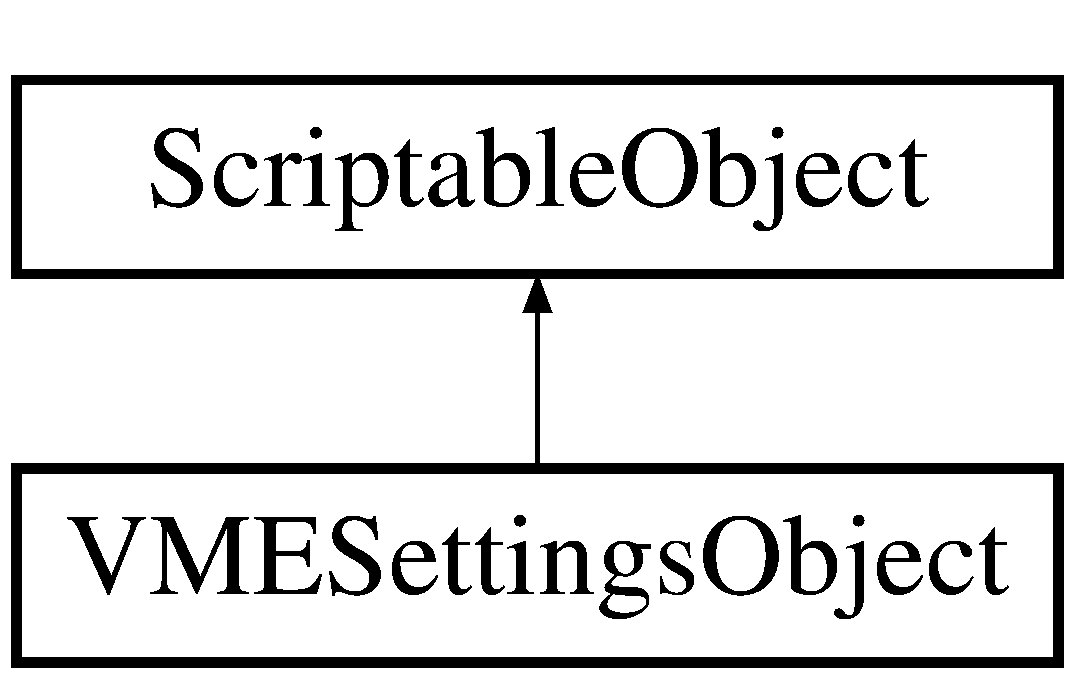
\includegraphics[height=2.000000cm]{class_v_m_e_settings_object}
\end{center}
\end{figure}
\subsection*{Public Member Functions}
\begin{DoxyCompactItemize}
\item 
void \hyperlink{class_v_m_e_settings_object_a8acba564b96c8d11c48119fa31ffa24b}{Restore\+To\+Factory\+Settings} ()
\begin{DoxyCompactList}\small\item\em Restores all settings to the default set by the creator. \end{DoxyCompactList}\end{DoxyCompactItemize}
\subsection*{Static Public Member Functions}
\begin{DoxyCompactItemize}
\item 
static \hyperlink{class_v_m_e_settings_object}{V\+M\+E\+Settings\+Object} \hyperlink{class_v_m_e_settings_object_a6e1b8fb3edc8c65774391cde2773cafa}{Load\+Scriptable\+Object} ()
\begin{DoxyCompactList}\small\item\em Gets the file located in the Project. \end{DoxyCompactList}\end{DoxyCompactItemize}
\subsection*{Public Attributes}
\begin{DoxyCompactItemize}
\item 
Key\+Code {\bfseries T\+O\+G\+G\+L\+E\+\_\+\+E\+D\+I\+T\+OR}\hypertarget{class_v_m_e_settings_object_af10d9ba9f0742bf067f191b605d29aae}{}\label{class_v_m_e_settings_object_af10d9ba9f0742bf067f191b605d29aae}

\item 
Key\+Code {\bfseries S\+H\+O\+W\+\_\+\+G\+R\+ID}\hypertarget{class_v_m_e_settings_object_ab66e84857309b514c3192e7a03bdc991}{}\label{class_v_m_e_settings_object_ab66e84857309b514c3192e7a03bdc991}

\item 
Key\+Code {\bfseries E\+N\+A\+B\+L\+E\+\_\+\+F\+I\+L\+E\+M\+A\+N\+A\+G\+ER}\hypertarget{class_v_m_e_settings_object_ad75067fc238b62e690ddf0841efab9c7}{}\label{class_v_m_e_settings_object_ad75067fc238b62e690ddf0841efab9c7}

\item 
Key\+Code {\bfseries E\+N\+A\+B\+L\+E\+\_\+\+S\+W\+A\+T\+CH}\hypertarget{class_v_m_e_settings_object_a0eae2f029a72b9d33127e680d4cc6e6c}{}\label{class_v_m_e_settings_object_a0eae2f029a72b9d33127e680d4cc6e6c}

\item 
Key\+Code {\bfseries E\+N\+A\+B\+L\+E\+\_\+\+S\+N\+AP}\hypertarget{class_v_m_e_settings_object_a12cfe16fd387974eb5879f76d3ecda2e}{}\label{class_v_m_e_settings_object_a12cfe16fd387974eb5879f76d3ecda2e}

\item 
Key\+Code {\bfseries E\+N\+A\+B\+L\+E\+\_\+\+M\+O\+DE}\hypertarget{class_v_m_e_settings_object_a2581343dea940a6516bafcd2a02333bf}{}\label{class_v_m_e_settings_object_a2581343dea940a6516bafcd2a02333bf}

\item 
Key\+Code {\bfseries E\+N\+A\+B\+L\+E\+\_\+\+C\+H\+U\+NK}\hypertarget{class_v_m_e_settings_object_a691a279a65ce047d9b939ab131c113ad}{}\label{class_v_m_e_settings_object_a691a279a65ce047d9b939ab131c113ad}

\item 
Key\+Code {\bfseries S\+E\+T\+\_\+\+M\+O\+D\+E\+\_\+\+T\+O\+\_\+\+S\+E\+L\+E\+CT}\hypertarget{class_v_m_e_settings_object_adc35cd06e0f07c5118ad57089e89d2ba}{}\label{class_v_m_e_settings_object_adc35cd06e0f07c5118ad57089e89d2ba}

\item 
Key\+Code {\bfseries S\+E\+T\+\_\+\+M\+O\+D\+E\+\_\+\+T\+O\+\_\+\+M\+O\+VE}\hypertarget{class_v_m_e_settings_object_aedaf25095866a6efb08b17c77c0f4a9b}{}\label{class_v_m_e_settings_object_aedaf25095866a6efb08b17c77c0f4a9b}

\item 
Key\+Code {\bfseries S\+E\+T\+\_\+\+M\+O\+D\+E\+\_\+\+T\+O\+\_\+\+P\+A\+I\+NT}\hypertarget{class_v_m_e_settings_object_a27f3b0427ad82d2c3dd23866e0b80dcf}{}\label{class_v_m_e_settings_object_a27f3b0427ad82d2c3dd23866e0b80dcf}

\item 
Key\+Code {\bfseries S\+E\+T\+\_\+\+M\+O\+D\+E\+\_\+\+T\+O\+\_\+\+E\+D\+IT}\hypertarget{class_v_m_e_settings_object_af58b6a95c4bc6f13f1faab0c70f3a378}{}\label{class_v_m_e_settings_object_af58b6a95c4bc6f13f1faab0c70f3a378}

\item 
Key\+Code {\bfseries S\+E\+T\+\_\+\+M\+O\+D\+E\+\_\+\+T\+O\+\_\+\+R\+E\+M\+O\+VE}\hypertarget{class_v_m_e_settings_object_a37cccb9978232ba4565d54e295bbd9a2}{}\label{class_v_m_e_settings_object_a37cccb9978232ba4565d54e295bbd9a2}

\item 
Key\+Code {\bfseries A\+P\+P\+L\+Y\+\_\+\+S\+I\+N\+G\+LE}\hypertarget{class_v_m_e_settings_object_a8417e9ce1f2ac45d4950af2e489954db}{}\label{class_v_m_e_settings_object_a8417e9ce1f2ac45d4950af2e489954db}

\item 
Key\+Code {\bfseries A\+P\+P\+L\+Y\+\_\+\+A\+LL}\hypertarget{class_v_m_e_settings_object_a8c445e98c2e89d302c37096b6d27da29}{}\label{class_v_m_e_settings_object_a8c445e98c2e89d302c37096b6d27da29}

\item 
Key\+Code {\bfseries R\+O\+T\+A\+T\+E\+\_\+\+T\+A\+R\+G\+ET}\hypertarget{class_v_m_e_settings_object_ae3ec868ef3bf1f4a03bc3a757282e245}{}\label{class_v_m_e_settings_object_ae3ec868ef3bf1f4a03bc3a757282e245}

\item 
Key\+Code {\bfseries C\+H\+A\+N\+G\+E\+B\+L\+O\+C\+K\+\_\+\+S\+T\+Y\+LE}\hypertarget{class_v_m_e_settings_object_a125387259cb3797d583175e9c3b4955e}{}\label{class_v_m_e_settings_object_a125387259cb3797d583175e9c3b4955e}

\item 
Key\+Code {\bfseries P\+I\+C\+K\+\_\+\+T\+I\+LE}\hypertarget{class_v_m_e_settings_object_a0e35743347f17acc1e2e49405b5c3682}{}\label{class_v_m_e_settings_object_a0e35743347f17acc1e2e49405b5c3682}

\item 
Key\+Code {\bfseries S\+W\+A\+T\+C\+H\+\_\+\+E\+N\+A\+B\+L\+E\+\_\+\+S\+E\+A\+R\+CH}\hypertarget{class_v_m_e_settings_object_a93b67ee22c6848b08ce3ccb7b7fc316a}{}\label{class_v_m_e_settings_object_a93b67ee22c6848b08ce3ccb7b7fc316a}

\item 
Key\+Code {\bfseries S\+W\+A\+T\+C\+H\+\_\+\+S\+E\+L\+E\+C\+T\+\_\+\+C\+A\+T\+E\+G\+O\+R\+Y\+\_\+\+D\+E\+C\+R\+E\+A\+SE}\hypertarget{class_v_m_e_settings_object_a088f34bd695050c42c973a2489ba365f}{}\label{class_v_m_e_settings_object_a088f34bd695050c42c973a2489ba365f}

\item 
Key\+Code {\bfseries S\+W\+A\+T\+C\+H\+\_\+\+S\+E\+L\+E\+C\+T\+\_\+\+C\+A\+T\+E\+G\+O\+R\+Y\+\_\+\+I\+N\+C\+R\+E\+A\+SE}\hypertarget{class_v_m_e_settings_object_aba6ca902d4ee04f41f9a1011b2e3ea25}{}\label{class_v_m_e_settings_object_aba6ca902d4ee04f41f9a1011b2e3ea25}

\item 
Key\+Code {\bfseries S\+W\+A\+T\+C\+H\+\_\+\+I\+T\+E\+M\+\_\+\+I\+N\+C\+R\+E\+A\+SE}\hypertarget{class_v_m_e_settings_object_afed7ef48b3c1f53ba995f637cf551a79}{}\label{class_v_m_e_settings_object_afed7ef48b3c1f53ba995f637cf551a79}

\item 
Key\+Code {\bfseries S\+W\+A\+T\+C\+H\+\_\+\+I\+T\+E\+M\+\_\+\+D\+E\+C\+R\+E\+A\+SE}\hypertarget{class_v_m_e_settings_object_a92488839f25effcc052a6b0ddedaade3}{}\label{class_v_m_e_settings_object_a92488839f25effcc052a6b0ddedaade3}

\end{DoxyCompactItemize}


\subsection{Detailed Description}
Holds all personal settings for the editor in a object inside the editor project. 



\subsection{Member Function Documentation}
\index{V\+M\+E\+Settings\+Object@{V\+M\+E\+Settings\+Object}!Load\+Scriptable\+Object@{Load\+Scriptable\+Object}}
\index{Load\+Scriptable\+Object@{Load\+Scriptable\+Object}!V\+M\+E\+Settings\+Object@{V\+M\+E\+Settings\+Object}}
\subsubsection[{\texorpdfstring{Load\+Scriptable\+Object()}{LoadScriptableObject()}}]{\setlength{\rightskip}{0pt plus 5cm}static {\bf V\+M\+E\+Settings\+Object} V\+M\+E\+Settings\+Object.\+Load\+Scriptable\+Object (
\begin{DoxyParamCaption}
{}
\end{DoxyParamCaption}
)\hspace{0.3cm}{\ttfamily [static]}}\hypertarget{class_v_m_e_settings_object_a6e1b8fb3edc8c65774391cde2773cafa}{}\label{class_v_m_e_settings_object_a6e1b8fb3edc8c65774391cde2773cafa}


Gets the file located in the Project. 

\begin{DoxyReturn}{Returns}
The Scriptable\+Object of type \hyperlink{class_v_m_e_settings_object}{V\+M\+E\+Settings\+Object}. 
\end{DoxyReturn}
\index{V\+M\+E\+Settings\+Object@{V\+M\+E\+Settings\+Object}!Restore\+To\+Factory\+Settings@{Restore\+To\+Factory\+Settings}}
\index{Restore\+To\+Factory\+Settings@{Restore\+To\+Factory\+Settings}!V\+M\+E\+Settings\+Object@{V\+M\+E\+Settings\+Object}}
\subsubsection[{\texorpdfstring{Restore\+To\+Factory\+Settings()}{RestoreToFactorySettings()}}]{\setlength{\rightskip}{0pt plus 5cm}void V\+M\+E\+Settings\+Object.\+Restore\+To\+Factory\+Settings (
\begin{DoxyParamCaption}
{}
\end{DoxyParamCaption}
)}\hypertarget{class_v_m_e_settings_object_a8acba564b96c8d11c48119fa31ffa24b}{}\label{class_v_m_e_settings_object_a8acba564b96c8d11c48119fa31ffa24b}


Restores all settings to the default set by the creator. 



The documentation for this class was generated from the following file\+:\begin{DoxyCompactItemize}
\item 
C\+:/\+Users/\+Kevin Breurken/\+Documents/\+Projects/\+V\+M\+E/\+Assets/\+V\+M\+E/\+Editor/\+Data/V\+M\+E\+Settings\+Object.\+cs\end{DoxyCompactItemize}

\hypertarget{class_v_m_e_1_1_settings_1_1_v_m_e_settings_window}{}\section{V\+M\+E.\+Settings.\+V\+M\+E\+Settings\+Window Class Reference}
\label{class_v_m_e_1_1_settings_1_1_v_m_e_settings_window}\index{V\+M\+E.\+Settings.\+V\+M\+E\+Settings\+Window@{V\+M\+E.\+Settings.\+V\+M\+E\+Settings\+Window}}
Inheritance diagram for V\+M\+E.\+Settings.\+V\+M\+E\+Settings\+Window\+:\begin{figure}[H]
\begin{center}
\leavevmode
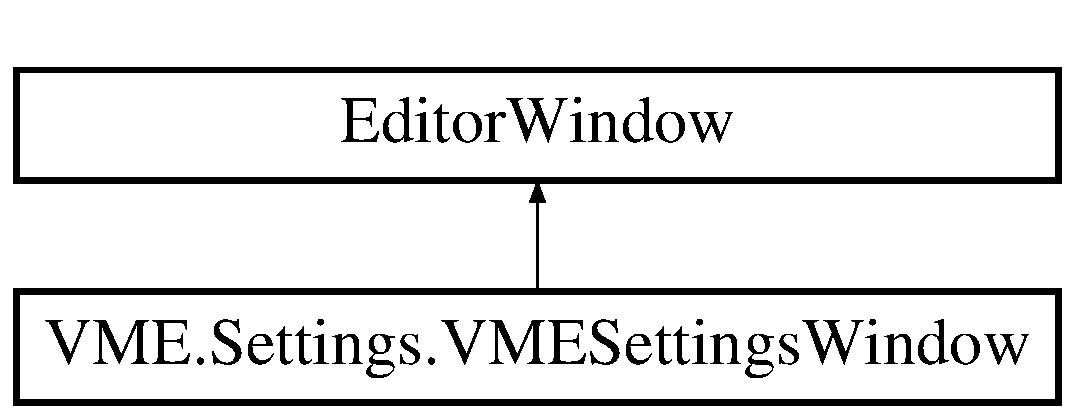
\includegraphics[height=2.000000cm]{class_v_m_e_1_1_settings_1_1_v_m_e_settings_window}
\end{center}
\end{figure}


The documentation for this class was generated from the following file\+:\begin{DoxyCompactItemize}
\item 
C\+:/\+Users/\+Kevin Breurken/\+Documents/\+Projects/\+V\+M\+E/\+Assets/\+V\+M\+E/\+Editor/\+Voxel\+Map\+Editor/\+Windows/V\+M\+E\+Settings\+Window.\+cs\end{DoxyCompactItemize}

\hypertarget{class_v_m_e_1_1_v_m_e_snap_panel}{}\section{V\+M\+E.\+V\+M\+E\+Snap\+Panel Class Reference}
\label{class_v_m_e_1_1_v_m_e_snap_panel}\index{V\+M\+E.\+V\+M\+E\+Snap\+Panel@{V\+M\+E.\+V\+M\+E\+Snap\+Panel}}


Voxel Map Snap Panel  


\subsection*{Public Member Functions}
\begin{DoxyCompactItemize}
\item 
void \hyperlink{class_v_m_e_1_1_v_m_e_snap_panel_ae1d34b15fee18534b9322de762345454}{Draw} ()
\begin{DoxyCompactList}\small\item\em Draws the snap panel. \end{DoxyCompactList}\item 
void \hyperlink{class_v_m_e_1_1_v_m_e_snap_panel_aa9fc552aea9e35017f48e53d38d9777b}{Input} ()
\begin{DoxyCompactList}\small\item\em Handles input for this \hyperlink{class_v_m_e_1_1_v_m_e_snap_panel}{V\+M\+E\+Snap\+Panel}. \end{DoxyCompactList}\end{DoxyCompactItemize}
\subsection*{Public Attributes}
\begin{DoxyCompactItemize}
\item 
bool \hyperlink{class_v_m_e_1_1_v_m_e_snap_panel_a8969f82f008fef4f0dfdc153f546330d}{position\+Snap\+Is\+Active}
\begin{DoxyCompactList}\small\item\em If position snap is enabled. \end{DoxyCompactList}\item 
bool \hyperlink{class_v_m_e_1_1_v_m_e_snap_panel_a77d0a41f559b90829555a64079f47ccf}{rotation\+Snap\+Is\+Active}
\begin{DoxyCompactList}\small\item\em If snap is enabled. \end{DoxyCompactList}\end{DoxyCompactItemize}


\subsection{Detailed Description}
Voxel Map Snap Panel 

Used for handling and drawing Snap related features. 

\subsection{Member Function Documentation}
\index{V\+M\+E\+::\+V\+M\+E\+Snap\+Panel@{V\+M\+E\+::\+V\+M\+E\+Snap\+Panel}!Draw@{Draw}}
\index{Draw@{Draw}!V\+M\+E\+::\+V\+M\+E\+Snap\+Panel@{V\+M\+E\+::\+V\+M\+E\+Snap\+Panel}}
\subsubsection[{\texorpdfstring{Draw()}{Draw()}}]{\setlength{\rightskip}{0pt plus 5cm}void V\+M\+E.\+V\+M\+E\+Snap\+Panel.\+Draw (
\begin{DoxyParamCaption}
{}
\end{DoxyParamCaption}
)}\hypertarget{class_v_m_e_1_1_v_m_e_snap_panel_ae1d34b15fee18534b9322de762345454}{}\label{class_v_m_e_1_1_v_m_e_snap_panel_ae1d34b15fee18534b9322de762345454}


Draws the snap panel. 

\index{V\+M\+E\+::\+V\+M\+E\+Snap\+Panel@{V\+M\+E\+::\+V\+M\+E\+Snap\+Panel}!Input@{Input}}
\index{Input@{Input}!V\+M\+E\+::\+V\+M\+E\+Snap\+Panel@{V\+M\+E\+::\+V\+M\+E\+Snap\+Panel}}
\subsubsection[{\texorpdfstring{Input()}{Input()}}]{\setlength{\rightskip}{0pt plus 5cm}void V\+M\+E.\+V\+M\+E\+Snap\+Panel.\+Input (
\begin{DoxyParamCaption}
{}
\end{DoxyParamCaption}
)}\hypertarget{class_v_m_e_1_1_v_m_e_snap_panel_aa9fc552aea9e35017f48e53d38d9777b}{}\label{class_v_m_e_1_1_v_m_e_snap_panel_aa9fc552aea9e35017f48e53d38d9777b}


Handles input for this \hyperlink{class_v_m_e_1_1_v_m_e_snap_panel}{V\+M\+E\+Snap\+Panel}. 



\subsection{Member Data Documentation}
\index{V\+M\+E\+::\+V\+M\+E\+Snap\+Panel@{V\+M\+E\+::\+V\+M\+E\+Snap\+Panel}!position\+Snap\+Is\+Active@{position\+Snap\+Is\+Active}}
\index{position\+Snap\+Is\+Active@{position\+Snap\+Is\+Active}!V\+M\+E\+::\+V\+M\+E\+Snap\+Panel@{V\+M\+E\+::\+V\+M\+E\+Snap\+Panel}}
\subsubsection[{\texorpdfstring{position\+Snap\+Is\+Active}{positionSnapIsActive}}]{\setlength{\rightskip}{0pt plus 5cm}bool V\+M\+E.\+V\+M\+E\+Snap\+Panel.\+position\+Snap\+Is\+Active}\hypertarget{class_v_m_e_1_1_v_m_e_snap_panel_a8969f82f008fef4f0dfdc153f546330d}{}\label{class_v_m_e_1_1_v_m_e_snap_panel_a8969f82f008fef4f0dfdc153f546330d}


If position snap is enabled. 

\index{V\+M\+E\+::\+V\+M\+E\+Snap\+Panel@{V\+M\+E\+::\+V\+M\+E\+Snap\+Panel}!rotation\+Snap\+Is\+Active@{rotation\+Snap\+Is\+Active}}
\index{rotation\+Snap\+Is\+Active@{rotation\+Snap\+Is\+Active}!V\+M\+E\+::\+V\+M\+E\+Snap\+Panel@{V\+M\+E\+::\+V\+M\+E\+Snap\+Panel}}
\subsubsection[{\texorpdfstring{rotation\+Snap\+Is\+Active}{rotationSnapIsActive}}]{\setlength{\rightskip}{0pt plus 5cm}bool V\+M\+E.\+V\+M\+E\+Snap\+Panel.\+rotation\+Snap\+Is\+Active}\hypertarget{class_v_m_e_1_1_v_m_e_snap_panel_a77d0a41f559b90829555a64079f47ccf}{}\label{class_v_m_e_1_1_v_m_e_snap_panel_a77d0a41f559b90829555a64079f47ccf}


If snap is enabled. 



The documentation for this class was generated from the following file\+:\begin{DoxyCompactItemize}
\item 
C\+:/\+Users/\+Kevin Breurken/\+Documents/\+Projects/\+V\+M\+E/\+Assets/\+V\+M\+E/\+Editor/\+Voxel\+Map\+Editor/\+Panels/\+Editor/V\+M\+E\+Snap\+Panel.\+cs\end{DoxyCompactItemize}

\hypertarget{class_v_m_e_tile_add_controls}{}\section{V\+M\+E\+Tile\+Add\+Controls Class Reference}
\label{class_v_m_e_tile_add_controls}\index{V\+M\+E\+Tile\+Add\+Controls@{V\+M\+E\+Tile\+Add\+Controls}}
\subsection*{Public Member Functions}
\begin{DoxyCompactItemize}
\item 
void \hyperlink{class_v_m_e_tile_add_controls_a4ad65e45e61a23bd9a39ef6a27097b6b}{Edit\+Tile} (Game\+Object \+\_\+tile\+To\+Create, Game\+Object \+\_\+tile\+To\+Remove)
\begin{DoxyCompactList}\small\item\em Edits a tile. \end{DoxyCompactList}\item 
void {\bfseries Paint\+T\+Ile} (Game\+Object \+\_\+tile\+To\+Create, Game\+Object \+\_\+hovered\+Tile, Vector3 \+\_\+position)\hypertarget{class_v_m_e_tile_add_controls_af302944f60e0b314a79e0ed8001e1434}{}\label{class_v_m_e_tile_add_controls_af302944f60e0b314a79e0ed8001e1434}

\end{DoxyCompactItemize}


\subsection{Member Function Documentation}
\index{V\+M\+E\+Tile\+Add\+Controls@{V\+M\+E\+Tile\+Add\+Controls}!Edit\+Tile@{Edit\+Tile}}
\index{Edit\+Tile@{Edit\+Tile}!V\+M\+E\+Tile\+Add\+Controls@{V\+M\+E\+Tile\+Add\+Controls}}
\subsubsection[{\texorpdfstring{Edit\+Tile(\+Game\+Object \+\_\+tile\+To\+Create, Game\+Object \+\_\+tile\+To\+Remove)}{EditTile(GameObject _tileToCreate, GameObject _tileToRemove)}}]{\setlength{\rightskip}{0pt plus 5cm}void V\+M\+E\+Tile\+Add\+Controls.\+Edit\+Tile (
\begin{DoxyParamCaption}
\item[{Game\+Object}]{\+\_\+tile\+To\+Create, }
\item[{Game\+Object}]{\+\_\+tile\+To\+Remove}
\end{DoxyParamCaption}
)}\hypertarget{class_v_m_e_tile_add_controls_a4ad65e45e61a23bd9a39ef6a27097b6b}{}\label{class_v_m_e_tile_add_controls_a4ad65e45e61a23bd9a39ef6a27097b6b}


Edits a tile. 


\begin{DoxyParams}{Parameters}
{\em \+\_\+tile\+To\+Create} & The tile that you want to create at selected position.\\
\hline
{\em \+\_\+tile\+To\+Remove} & The tile that you want to remove.\\
\hline
\end{DoxyParams}


The documentation for this class was generated from the following file\+:\begin{DoxyCompactItemize}
\item 
C\+:/\+Users/\+Kevin Breurken/\+Documents/\+Projects/\+V\+M\+E/\+Assets/\+V\+M\+E/\+Editor/\+Voxel\+Map\+Editor/\+Controls/V\+M\+E\+Tile\+Add\+Controls.\+cs\end{DoxyCompactItemize}

\hypertarget{class_v_m_e_1_1_v_m_e_voxel_swatch_panel}{}\section{V\+M\+E.\+V\+M\+E\+Voxel\+Swatch\+Panel Class Reference}
\label{class_v_m_e_1_1_v_m_e_voxel_swatch_panel}\index{V\+M\+E.\+V\+M\+E\+Voxel\+Swatch\+Panel@{V\+M\+E.\+V\+M\+E\+Voxel\+Swatch\+Panel}}
Inheritance diagram for V\+M\+E.\+V\+M\+E\+Voxel\+Swatch\+Panel\+:\begin{figure}[H]
\begin{center}
\leavevmode
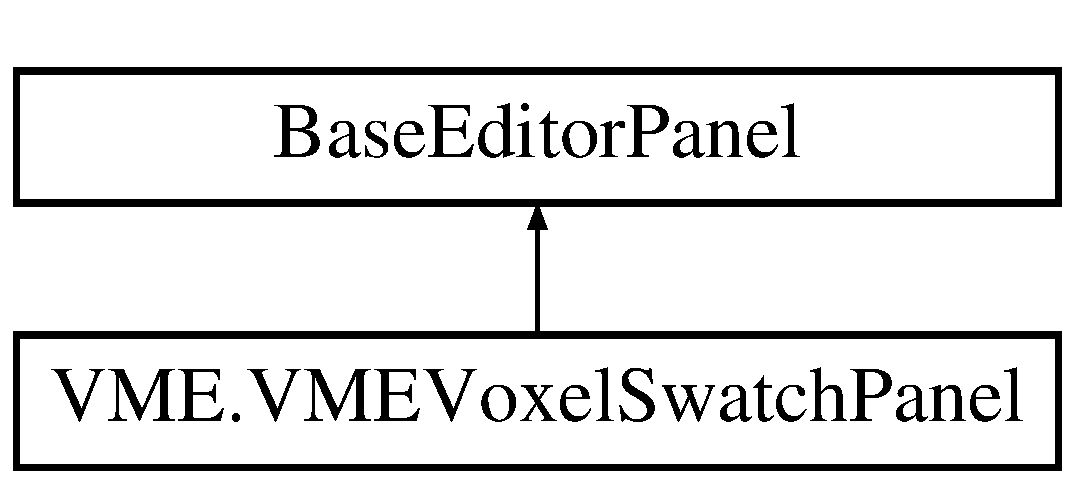
\includegraphics[height=2.000000cm]{class_v_m_e_1_1_v_m_e_voxel_swatch_panel}
\end{center}
\end{figure}
\subsection*{Public Member Functions}
\begin{DoxyCompactItemize}
\item 
{\bfseries V\+M\+E\+Voxel\+Swatch\+Panel} (Editor\+Window \+\_\+window, Key\+Code \+\_\+toggle\+Key)\hypertarget{class_v_m_e_1_1_v_m_e_voxel_swatch_panel_aa3783e3c8bcbc0336213ff4101f93996}{}\label{class_v_m_e_1_1_v_m_e_voxel_swatch_panel_aa3783e3c8bcbc0336213ff4101f93996}

\item 
override void \hyperlink{class_v_m_e_1_1_v_m_e_voxel_swatch_panel_a1756e7e5d376e59d966b26d21c9e9d3c}{On\+Opened} ()
\begin{DoxyCompactList}\small\item\em Called when the panel is opened. \end{DoxyCompactList}\item 
override void \hyperlink{class_v_m_e_1_1_v_m_e_voxel_swatch_panel_a663cd8478cdcb41c20fc9078f893c3a0}{Draw\+Content} ()
\begin{DoxyCompactList}\small\item\em Draws the content of the panel. \end{DoxyCompactList}\item 
override void \hyperlink{class_v_m_e_1_1_v_m_e_voxel_swatch_panel_a4c94c74221d96e48ed17ecb6b2a98ffb}{Input} (Scene\+View scene\+View)
\begin{DoxyCompactList}\small\item\em Used for handling keyboard input. \end{DoxyCompactList}\item 
void \hyperlink{class_v_m_e_1_1_v_m_e_voxel_swatch_panel_a19fcb070e3d6a3a61ce75602b9476bf6}{Set\+Voxel\+Swatch} (\hyperlink{class_voxel_swatch}{Voxel\+Swatch} \+\_\+swatch)
\begin{DoxyCompactList}\small\item\em Sets a new \hyperlink{class_voxel_swatch}{Voxel\+Swatch}. \end{DoxyCompactList}\item 
void {\bfseries Set\+Category} (int category\+Index)\hypertarget{class_v_m_e_1_1_v_m_e_voxel_swatch_panel_a975a8484811df2ac0c92f47156a4ccc4}{}\label{class_v_m_e_1_1_v_m_e_voxel_swatch_panel_a975a8484811df2ac0c92f47156a4ccc4}

\item 
string {\bfseries Get\+Category\+Name} ()\hypertarget{class_v_m_e_1_1_v_m_e_voxel_swatch_panel_af47fc820fffad77b296ff0b740073c44}{}\label{class_v_m_e_1_1_v_m_e_voxel_swatch_panel_af47fc820fffad77b296ff0b740073c44}

\item 
void {\bfseries Set\+Swatch\+Selection} (Game\+Object obj)\hypertarget{class_v_m_e_1_1_v_m_e_voxel_swatch_panel_aea081c7e7bcce5f838f249a1592a5af0}{}\label{class_v_m_e_1_1_v_m_e_voxel_swatch_panel_aea081c7e7bcce5f838f249a1592a5af0}

\item 
Game\+Object \hyperlink{class_v_m_e_1_1_v_m_e_voxel_swatch_panel_ac3934594ea3b321dcca43af6bf4a2422}{Get\+Selected\+Tile} ()
\begin{DoxyCompactList}\small\item\em Returns the item that is selected in this Swatch\+Panel. \end{DoxyCompactList}\item 
\hyperlink{class_voxel_swatch}{Voxel\+Swatch} {\bfseries Get\+Swatch} ()\hypertarget{class_v_m_e_1_1_v_m_e_voxel_swatch_panel_a80099d926458c52438e617ea7fb98618}{}\label{class_v_m_e_1_1_v_m_e_voxel_swatch_panel_a80099d926458c52438e617ea7fb98618}

\end{DoxyCompactItemize}
\subsection*{Additional Inherited Members}


\subsection{Member Function Documentation}
\index{V\+M\+E\+::\+V\+M\+E\+Voxel\+Swatch\+Panel@{V\+M\+E\+::\+V\+M\+E\+Voxel\+Swatch\+Panel}!Draw\+Content@{Draw\+Content}}
\index{Draw\+Content@{Draw\+Content}!V\+M\+E\+::\+V\+M\+E\+Voxel\+Swatch\+Panel@{V\+M\+E\+::\+V\+M\+E\+Voxel\+Swatch\+Panel}}
\subsubsection[{\texorpdfstring{Draw\+Content()}{DrawContent()}}]{\setlength{\rightskip}{0pt plus 5cm}override void V\+M\+E.\+V\+M\+E\+Voxel\+Swatch\+Panel.\+Draw\+Content (
\begin{DoxyParamCaption}
{}
\end{DoxyParamCaption}
)\hspace{0.3cm}{\ttfamily [virtual]}}\hypertarget{class_v_m_e_1_1_v_m_e_voxel_swatch_panel_a663cd8478cdcb41c20fc9078f893c3a0}{}\label{class_v_m_e_1_1_v_m_e_voxel_swatch_panel_a663cd8478cdcb41c20fc9078f893c3a0}


Draws the content of the panel. 



Reimplemented from \hyperlink{class_base_editor_panel_a96ea35bdda7a8e955baa1fd21635bffa}{Base\+Editor\+Panel}.

\index{V\+M\+E\+::\+V\+M\+E\+Voxel\+Swatch\+Panel@{V\+M\+E\+::\+V\+M\+E\+Voxel\+Swatch\+Panel}!Get\+Selected\+Tile@{Get\+Selected\+Tile}}
\index{Get\+Selected\+Tile@{Get\+Selected\+Tile}!V\+M\+E\+::\+V\+M\+E\+Voxel\+Swatch\+Panel@{V\+M\+E\+::\+V\+M\+E\+Voxel\+Swatch\+Panel}}
\subsubsection[{\texorpdfstring{Get\+Selected\+Tile()}{GetSelectedTile()}}]{\setlength{\rightskip}{0pt plus 5cm}Game\+Object V\+M\+E.\+V\+M\+E\+Voxel\+Swatch\+Panel.\+Get\+Selected\+Tile (
\begin{DoxyParamCaption}
{}
\end{DoxyParamCaption}
)}\hypertarget{class_v_m_e_1_1_v_m_e_voxel_swatch_panel_ac3934594ea3b321dcca43af6bf4a2422}{}\label{class_v_m_e_1_1_v_m_e_voxel_swatch_panel_ac3934594ea3b321dcca43af6bf4a2422}


Returns the item that is selected in this Swatch\+Panel. 

\begin{DoxyReturn}{Returns}
Item selected
\end{DoxyReturn}
\index{V\+M\+E\+::\+V\+M\+E\+Voxel\+Swatch\+Panel@{V\+M\+E\+::\+V\+M\+E\+Voxel\+Swatch\+Panel}!Input@{Input}}
\index{Input@{Input}!V\+M\+E\+::\+V\+M\+E\+Voxel\+Swatch\+Panel@{V\+M\+E\+::\+V\+M\+E\+Voxel\+Swatch\+Panel}}
\subsubsection[{\texorpdfstring{Input(\+Scene\+View scene\+View)}{Input(SceneView sceneView)}}]{\setlength{\rightskip}{0pt plus 5cm}override void V\+M\+E.\+V\+M\+E\+Voxel\+Swatch\+Panel.\+Input (
\begin{DoxyParamCaption}
\item[{Scene\+View}]{\+\_\+scene\+View}
\end{DoxyParamCaption}
)\hspace{0.3cm}{\ttfamily [virtual]}}\hypertarget{class_v_m_e_1_1_v_m_e_voxel_swatch_panel_a4c94c74221d96e48ed17ecb6b2a98ffb}{}\label{class_v_m_e_1_1_v_m_e_voxel_swatch_panel_a4c94c74221d96e48ed17ecb6b2a98ffb}


Used for handling keyboard input. 



Reimplemented from \hyperlink{class_base_editor_panel_a9bd01437be0e246418dc89209ef2125b}{Base\+Editor\+Panel}.

\index{V\+M\+E\+::\+V\+M\+E\+Voxel\+Swatch\+Panel@{V\+M\+E\+::\+V\+M\+E\+Voxel\+Swatch\+Panel}!On\+Opened@{On\+Opened}}
\index{On\+Opened@{On\+Opened}!V\+M\+E\+::\+V\+M\+E\+Voxel\+Swatch\+Panel@{V\+M\+E\+::\+V\+M\+E\+Voxel\+Swatch\+Panel}}
\subsubsection[{\texorpdfstring{On\+Opened()}{OnOpened()}}]{\setlength{\rightskip}{0pt plus 5cm}override void V\+M\+E.\+V\+M\+E\+Voxel\+Swatch\+Panel.\+On\+Opened (
\begin{DoxyParamCaption}
{}
\end{DoxyParamCaption}
)\hspace{0.3cm}{\ttfamily [virtual]}}\hypertarget{class_v_m_e_1_1_v_m_e_voxel_swatch_panel_a1756e7e5d376e59d966b26d21c9e9d3c}{}\label{class_v_m_e_1_1_v_m_e_voxel_swatch_panel_a1756e7e5d376e59d966b26d21c9e9d3c}


Called when the panel is opened. 



Reimplemented from \hyperlink{class_base_editor_panel_a3a8ccb88e5e34920880e9000a48fb862}{Base\+Editor\+Panel}.

\index{V\+M\+E\+::\+V\+M\+E\+Voxel\+Swatch\+Panel@{V\+M\+E\+::\+V\+M\+E\+Voxel\+Swatch\+Panel}!Set\+Voxel\+Swatch@{Set\+Voxel\+Swatch}}
\index{Set\+Voxel\+Swatch@{Set\+Voxel\+Swatch}!V\+M\+E\+::\+V\+M\+E\+Voxel\+Swatch\+Panel@{V\+M\+E\+::\+V\+M\+E\+Voxel\+Swatch\+Panel}}
\subsubsection[{\texorpdfstring{Set\+Voxel\+Swatch(\+Voxel\+Swatch \+\_\+swatch)}{SetVoxelSwatch(VoxelSwatch _swatch)}}]{\setlength{\rightskip}{0pt plus 5cm}void V\+M\+E.\+V\+M\+E\+Voxel\+Swatch\+Panel.\+Set\+Voxel\+Swatch (
\begin{DoxyParamCaption}
\item[{{\bf Voxel\+Swatch}}]{\+\_\+swatch}
\end{DoxyParamCaption}
)}\hypertarget{class_v_m_e_1_1_v_m_e_voxel_swatch_panel_a19fcb070e3d6a3a61ce75602b9476bf6}{}\label{class_v_m_e_1_1_v_m_e_voxel_swatch_panel_a19fcb070e3d6a3a61ce75602b9476bf6}


Sets a new \hyperlink{class_voxel_swatch}{Voxel\+Swatch}. 


\begin{DoxyParams}{Parameters}
{\em \+\_\+swatch} & The Swatch\\
\hline
\end{DoxyParams}


The documentation for this class was generated from the following file\+:\begin{DoxyCompactItemize}
\item 
C\+:/\+Users/\+Kevin Breurken/\+Documents/\+Projects/\+V\+M\+E/\+Assets/\+V\+M\+E/\+Editor/\+Voxel\+Map\+Editor/\+Panels/\+Editor/V\+M\+E\+Voxel\+Swatch\+Panel.\+cs\end{DoxyCompactItemize}

\hypertarget{class_voxel_map}{}\section{Voxel\+Map Class Reference}
\label{class_voxel_map}\index{Voxel\+Map@{Voxel\+Map}}
Inheritance diagram for Voxel\+Map\+:\begin{figure}[H]
\begin{center}
\leavevmode
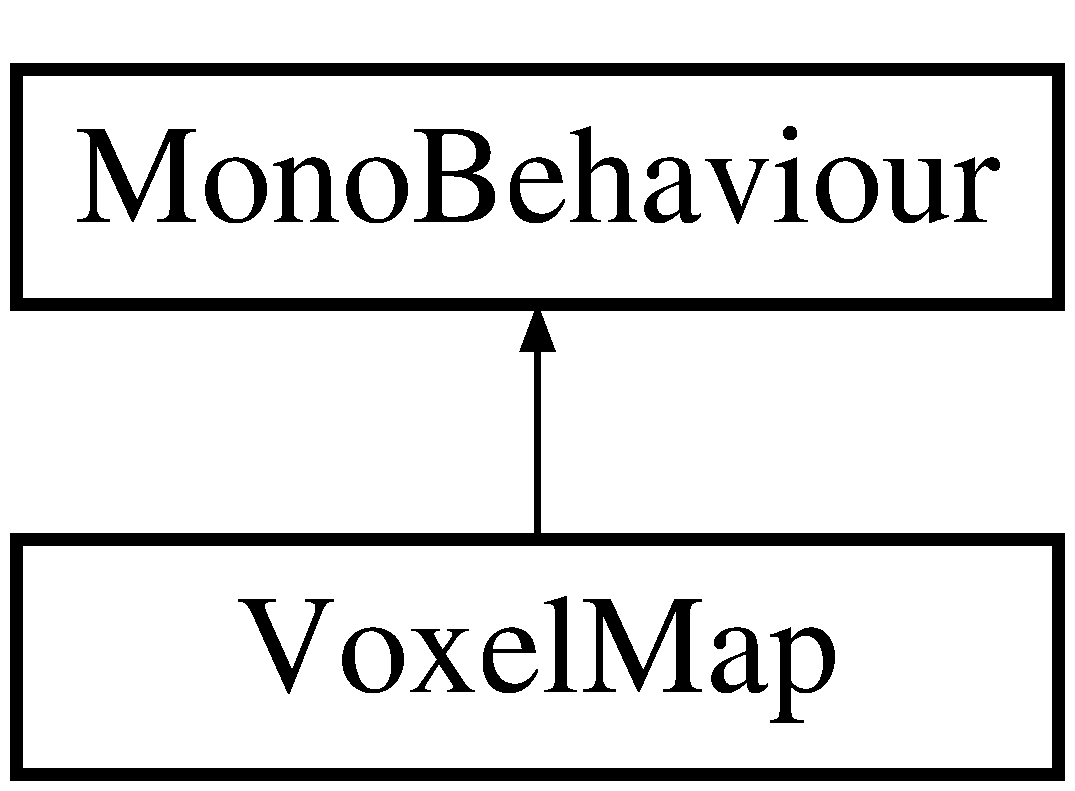
\includegraphics[height=2.000000cm]{class_voxel_map}
\end{center}
\end{figure}
\subsection*{Public Attributes}
\begin{DoxyCompactItemize}
\item 
\hyperlink{class_voxel_swatch}{Voxel\+Swatch} {\bfseries voxel\+Swatch}\hypertarget{class_voxel_map_a982b16765614119d196c7279bc8d35d6}{}\label{class_voxel_map_a982b16765614119d196c7279bc8d35d6}

\item 
\hyperlink{class_chunk_spawner}{Chunk\+Spawner}\mbox{[}$\,$\mbox{]} {\bfseries chunks}\hypertarget{class_voxel_map_a78645e12f52fb1fa2415b059165ca3f6}{}\label{class_voxel_map_a78645e12f52fb1fa2415b059165ca3f6}

\end{DoxyCompactItemize}


The documentation for this class was generated from the following file\+:\begin{DoxyCompactItemize}
\item 
C\+:/\+Users/\+Kevin Breurken/\+Documents/\+Projects/\+V\+M\+E/\+Assets/\+V\+M\+E/\+Scripts/Voxel\+Map.\+cs\end{DoxyCompactItemize}

\hypertarget{class_voxel_swatch}{}\section{Voxel\+Swatch Class Reference}
\label{class_voxel_swatch}\index{Voxel\+Swatch@{Voxel\+Swatch}}
Inheritance diagram for Voxel\+Swatch\+:\begin{figure}[H]
\begin{center}
\leavevmode
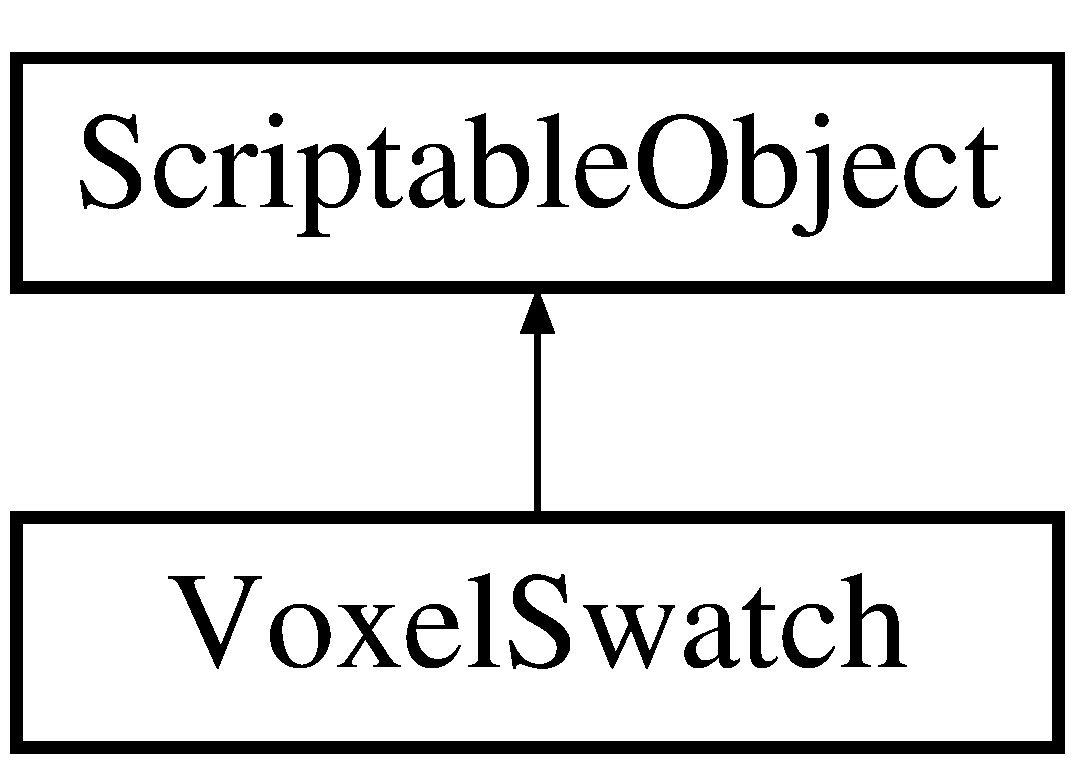
\includegraphics[height=2.000000cm]{class_voxel_swatch}
\end{center}
\end{figure}
\subsection*{Public Attributes}
\begin{DoxyCompactItemize}
\item 
List$<$ \hyperlink{class_v_s_category}{V\+S\+Category} $>$ {\bfseries categories}\hypertarget{class_voxel_swatch_a658229ce22f249508cf21ad66622d1ec}{}\label{class_voxel_swatch_a658229ce22f249508cf21ad66622d1ec}

\item 
List$<$ \hyperlink{class_quick_reference}{Quick\+Reference} $>$ {\bfseries references}\hypertarget{class_voxel_swatch_a3bdd5a603812d1cc8fb0f9c493b498e4}{}\label{class_voxel_swatch_a3bdd5a603812d1cc8fb0f9c493b498e4}

\end{DoxyCompactItemize}


The documentation for this class was generated from the following file\+:\begin{DoxyCompactItemize}
\item 
C\+:/\+Users/\+Kevin Breurken/\+Documents/\+Projects/\+V\+M\+E/\+Assets/\+V\+M\+E/\+Scripts/Voxel\+Swatch.\+cs\end{DoxyCompactItemize}

\hypertarget{class_v_s_category}{}\section{V\+S\+Category Class Reference}
\label{class_v_s_category}\index{V\+S\+Category@{V\+S\+Category}}
\subsection*{Public Member Functions}
\begin{DoxyCompactItemize}
\item 
{\bfseries V\+S\+Category} (string \+\_\+name)\hypertarget{class_v_s_category_a6db0268109430e32946e1b881e25fb1e}{}\label{class_v_s_category_a6db0268109430e32946e1b881e25fb1e}

\item 
void {\bfseries Add} (List$<$ \hyperlink{class_quick_reference}{Quick\+Reference} $>$ \+\_\+reference, Game\+Object \+\_\+object, string \+\_\+groupname, int \+\_\+index)\hypertarget{class_v_s_category_ab47fe555eaf0001bff285bc0742e97ec}{}\label{class_v_s_category_ab47fe555eaf0001bff285bc0742e97ec}

\end{DoxyCompactItemize}
\subsection*{Public Attributes}
\begin{DoxyCompactItemize}
\item 
string {\bfseries name}\hypertarget{class_v_s_category_a62c882e1acf517e40f95da21742b55ea}{}\label{class_v_s_category_a62c882e1acf517e40f95da21742b55ea}

\item 
List$<$ \hyperlink{class_v_s_item_group}{V\+S\+Item\+Group} $>$ {\bfseries tilegroups}\hypertarget{class_v_s_category_a007f1f04b040d03bf86e0c5a0c5d9cd2}{}\label{class_v_s_category_a007f1f04b040d03bf86e0c5a0c5d9cd2}

\end{DoxyCompactItemize}


The documentation for this class was generated from the following file\+:\begin{DoxyCompactItemize}
\item 
C\+:/\+Users/\+Kevin Breurken/\+Documents/\+Projects/\+V\+M\+E/\+Assets/\+V\+M\+E/\+Scripts/Voxel\+Swatch.\+cs\end{DoxyCompactItemize}

\hypertarget{class_v_s_e_header}{}\section{V\+S\+E\+Header Class Reference}
\label{class_v_s_e_header}\index{V\+S\+E\+Header@{V\+S\+E\+Header}}


Contains the Swatch input field and category selection buttons  


Inheritance diagram for V\+S\+E\+Header\+:\begin{figure}[H]
\begin{center}
\leavevmode
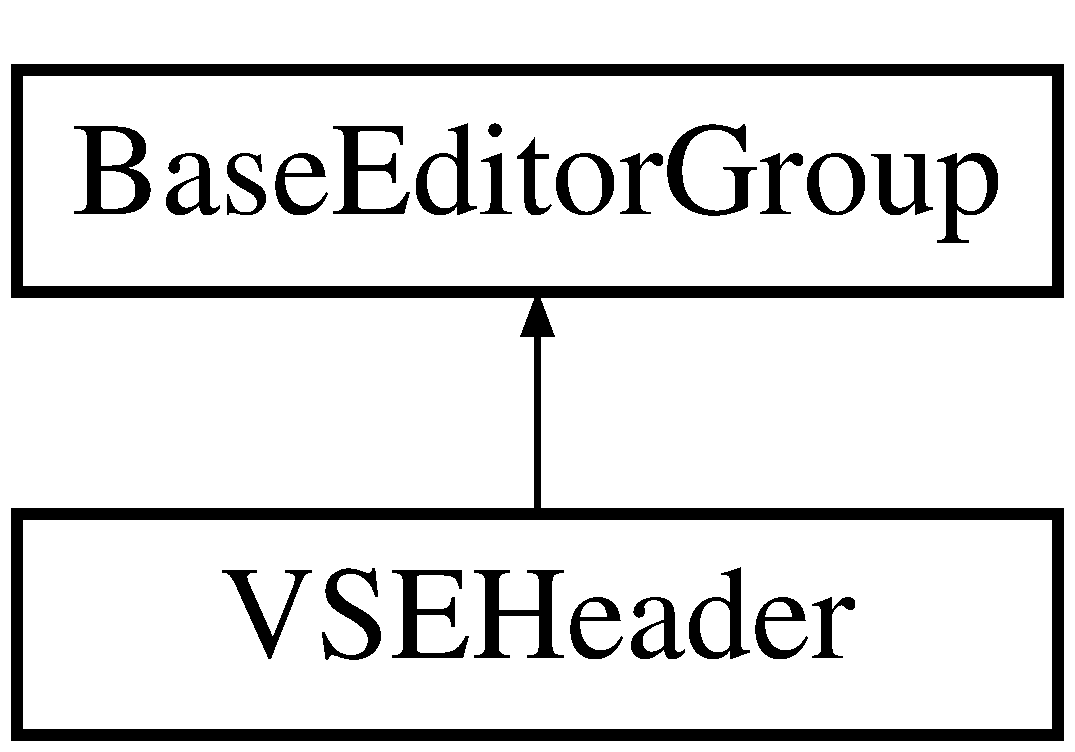
\includegraphics[height=2.000000cm]{class_v_s_e_header}
\end{center}
\end{figure}
\subsection*{Public Types}
\begin{DoxyCompactItemize}
\item 
enum {\bfseries Selected\+Category\+State} \{ \\*
{\bfseries No\+Swatch\+Selected}, 
{\bfseries None}, 
{\bfseries General}, 
{\bfseries Swatch}, 
\\*
{\bfseries Etc}
 \}\hypertarget{class_v_s_e_header_a2ed21466f35821439e8d8e2cca94381a}{}\label{class_v_s_e_header_a2ed21466f35821439e8d8e2cca94381a}

\end{DoxyCompactItemize}
\subsection*{Public Member Functions}
\begin{DoxyCompactItemize}
\item 
delegate void {\bfseries Voxel\+Swatch\+Action} (\hyperlink{class_voxel_swatch}{Voxel\+Swatch} \+\_\+swatch)\hypertarget{class_v_s_e_header_a7181bf17ebc70c90620ca9e4e7a679b5}{}\label{class_v_s_e_header_a7181bf17ebc70c90620ca9e4e7a679b5}

\item 
delegate void {\bfseries Category\+Switch\+Action} (Selected\+Category\+State \+\_\+state)\hypertarget{class_v_s_e_header_a701bc298aa2c2d6e552d33bfbd1cd495}{}\label{class_v_s_e_header_a701bc298aa2c2d6e552d33bfbd1cd495}

\item 
{\bfseries V\+S\+E\+Header} (Editor\+Window \+\_\+window)\hypertarget{class_v_s_e_header_ac43871f65cffd7378b7f92753f54d35d}{}\label{class_v_s_e_header_ac43871f65cffd7378b7f92753f54d35d}

\item 
override void \hyperlink{class_v_s_e_header_ac866415e77168e78f59965f3a61a0e64}{Draw\+Content} ()
\begin{DoxyCompactList}\small\item\em Draws the content of the panel. \end{DoxyCompactList}\end{DoxyCompactItemize}
\subsection*{Public Attributes}
\begin{DoxyCompactItemize}
\item 
Selected\+Category\+State {\bfseries current\+State} = Selected\+Category\+State.\+No\+Swatch\+Selected\hypertarget{class_v_s_e_header_ae6542a2ef5fba7ebd929bd8d0c9c7dac}{}\label{class_v_s_e_header_ae6542a2ef5fba7ebd929bd8d0c9c7dac}

\item 
\hyperlink{class_voxel_swatch}{Voxel\+Swatch} {\bfseries voxel\+Swatch}\hypertarget{class_v_s_e_header_a428ff88cfcafe14c61962451d4b0005b}{}\label{class_v_s_e_header_a428ff88cfcafe14c61962451d4b0005b}

\end{DoxyCompactItemize}
\subsection*{Events}
\begin{DoxyCompactItemize}
\item 
Voxel\+Swatch\+Action {\bfseries On\+Voxel\+Swatch\+Changed\+Event}\hypertarget{class_v_s_e_header_acb7a996a06c216320c487be34bff94a9}{}\label{class_v_s_e_header_acb7a996a06c216320c487be34bff94a9}

\item 
Category\+Switch\+Action {\bfseries On\+Header\+Category\+Switched}\hypertarget{class_v_s_e_header_ae699aa43d5904cb6bbe804ff9b9c0b69}{}\label{class_v_s_e_header_ae699aa43d5904cb6bbe804ff9b9c0b69}

\end{DoxyCompactItemize}


\subsection{Detailed Description}
Contains the Swatch input field and category selection buttons 



\subsection{Member Function Documentation}
\index{V\+S\+E\+Header@{V\+S\+E\+Header}!Draw\+Content@{Draw\+Content}}
\index{Draw\+Content@{Draw\+Content}!V\+S\+E\+Header@{V\+S\+E\+Header}}
\subsubsection[{\texorpdfstring{Draw\+Content()}{DrawContent()}}]{\setlength{\rightskip}{0pt plus 5cm}override void V\+S\+E\+Header.\+Draw\+Content (
\begin{DoxyParamCaption}
{}
\end{DoxyParamCaption}
)\hspace{0.3cm}{\ttfamily [virtual]}}\hypertarget{class_v_s_e_header_ac866415e77168e78f59965f3a61a0e64}{}\label{class_v_s_e_header_ac866415e77168e78f59965f3a61a0e64}


Draws the content of the panel. 



Reimplemented from \hyperlink{class_base_editor_group_a8a41e2753ba3c316a1c7fe35ef21897c}{Base\+Editor\+Group}.



The documentation for this class was generated from the following file\+:\begin{DoxyCompactItemize}
\item 
C\+:/\+Users/\+Kevin Breurken/\+Documents/\+Projects/\+V\+M\+E/\+Assets/\+V\+M\+E/\+Editor/\+Voxel\+Swatch\+Editor/\+Panels/V\+S\+E\+Header.\+cs\end{DoxyCompactItemize}

\hypertarget{class_v_s_e_1_1_v_s_e_window}{}\section{V\+S\+E.\+V\+S\+E\+Window Class Reference}
\label{class_v_s_e_1_1_v_s_e_window}\index{V\+S\+E.\+V\+S\+E\+Window@{V\+S\+E.\+V\+S\+E\+Window}}
Inheritance diagram for V\+S\+E.\+V\+S\+E\+Window\+:\begin{figure}[H]
\begin{center}
\leavevmode
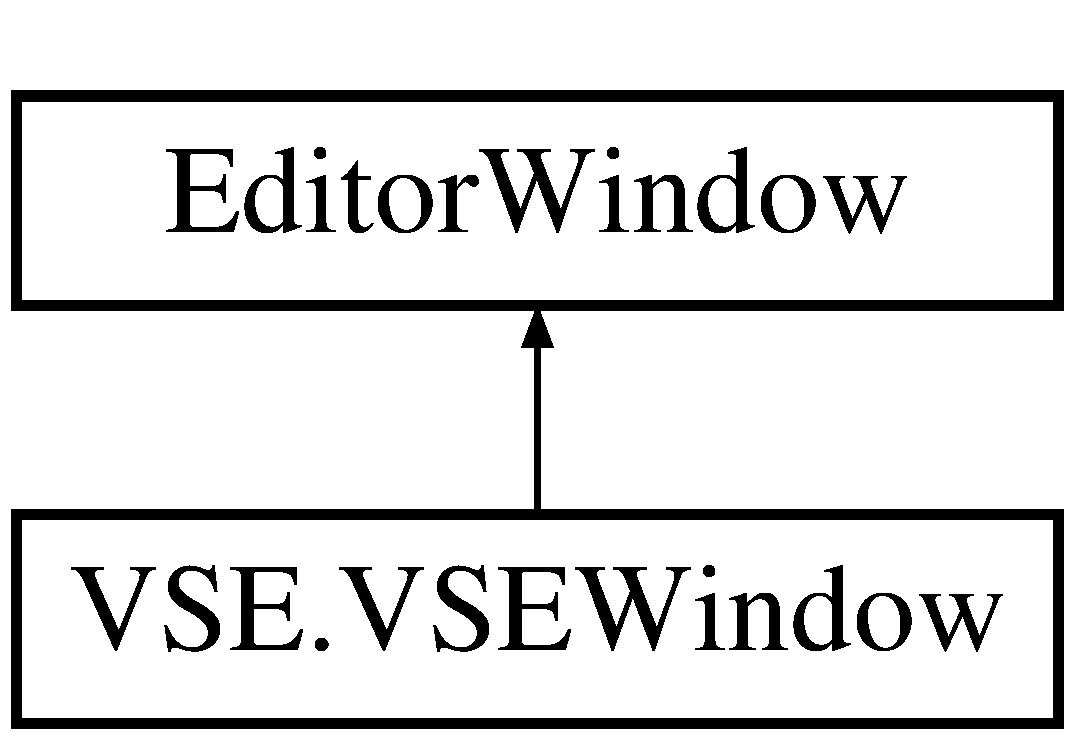
\includegraphics[height=2.000000cm]{class_v_s_e_1_1_v_s_e_window}
\end{center}
\end{figure}
\subsection*{Public Member Functions}
\begin{DoxyCompactItemize}
\item 
void \hyperlink{class_v_s_e_1_1_v_s_e_window_a3c82a480fd6c38b68caec54e7943a322}{Update} ()
\begin{DoxyCompactList}\small\item\em For repainting the Window. \end{DoxyCompactList}\end{DoxyCompactItemize}
\subsection*{Static Public Attributes}
\begin{DoxyCompactItemize}
\item 
static \hyperlink{class_v_s_e_header}{V\+S\+E\+Header} {\bfseries header}\hypertarget{class_v_s_e_1_1_v_s_e_window_a37871719cb2069fe48e772de7c5b4a4c}{}\label{class_v_s_e_1_1_v_s_e_window_a37871719cb2069fe48e772de7c5b4a4c}

\end{DoxyCompactItemize}
\subsection*{Properties}
\begin{DoxyCompactItemize}
\item 
static \hyperlink{class_v_s_e_1_1_v_s_e_window}{V\+S\+E\+Window} {\bfseries Instance}\hspace{0.3cm}{\ttfamily  \mbox{[}get\mbox{]}}\hypertarget{class_v_s_e_1_1_v_s_e_window_aa825c1d4f7eaf9ea047811d6a7ca4718}{}\label{class_v_s_e_1_1_v_s_e_window_aa825c1d4f7eaf9ea047811d6a7ca4718}

\end{DoxyCompactItemize}


\subsection{Member Function Documentation}
\index{V\+S\+E\+::\+V\+S\+E\+Window@{V\+S\+E\+::\+V\+S\+E\+Window}!Update@{Update}}
\index{Update@{Update}!V\+S\+E\+::\+V\+S\+E\+Window@{V\+S\+E\+::\+V\+S\+E\+Window}}
\subsubsection[{\texorpdfstring{Update()}{Update()}}]{\setlength{\rightskip}{0pt plus 5cm}void V\+S\+E.\+V\+S\+E\+Window.\+Update (
\begin{DoxyParamCaption}
{}
\end{DoxyParamCaption}
)}\hypertarget{class_v_s_e_1_1_v_s_e_window_a3c82a480fd6c38b68caec54e7943a322}{}\label{class_v_s_e_1_1_v_s_e_window_a3c82a480fd6c38b68caec54e7943a322}


For repainting the Window. 



The documentation for this class was generated from the following file\+:\begin{DoxyCompactItemize}
\item 
C\+:/\+Users/\+Kevin Breurken/\+Documents/\+Projects/\+V\+M\+E/\+Assets/\+V\+M\+E/\+Editor/\+Voxel\+Swatch\+Editor/\+Window/V\+S\+E\+Window.\+cs\end{DoxyCompactItemize}

\hypertarget{class_v_s_item_group}{}\section{V\+S\+Item\+Group Class Reference}
\label{class_v_s_item_group}\index{V\+S\+Item\+Group@{V\+S\+Item\+Group}}
\subsection*{Public Member Functions}
\begin{DoxyCompactItemize}
\item 
{\bfseries V\+S\+Item\+Group} (string \+\_\+name, string \+\_\+category\+Name)\hypertarget{class_v_s_item_group_ae1fdef37c6094bacb9cc725684520d3f}{}\label{class_v_s_item_group_ae1fdef37c6094bacb9cc725684520d3f}

\item 
void {\bfseries Add} (List$<$ \hyperlink{class_quick_reference}{Quick\+Reference} $>$ \+\_\+reference, Game\+Object \+\_\+object, string \+\_\+category\+Name, int \+\_\+name)\hypertarget{class_v_s_item_group_a02bafc4f989b0ecc0939ddafdee6fddb}{}\label{class_v_s_item_group_a02bafc4f989b0ecc0939ddafdee6fddb}

\end{DoxyCompactItemize}
\subsection*{Public Attributes}
\begin{DoxyCompactItemize}
\item 
string {\bfseries name}\hypertarget{class_v_s_item_group_a15d7a20bec635daf71c616eb4ecf0feb}{}\label{class_v_s_item_group_a15d7a20bec635daf71c616eb4ecf0feb}

\item 
string {\bfseries category\+Name}\hypertarget{class_v_s_item_group_ad30fcd95dcb4cdbea4a1cd875be014f4}{}\label{class_v_s_item_group_ad30fcd95dcb4cdbea4a1cd875be014f4}

\item 
List$<$ Game\+Object $>$ {\bfseries tiles}\hypertarget{class_v_s_item_group_a4c800fffecc7fb129255e8f9f95375a7}{}\label{class_v_s_item_group_a4c800fffecc7fb129255e8f9f95375a7}

\end{DoxyCompactItemize}


The documentation for this class was generated from the following file\+:\begin{DoxyCompactItemize}
\item 
C\+:/\+Users/\+Kevin Breurken/\+Documents/\+Projects/\+V\+M\+E/\+Assets/\+V\+M\+E/\+Scripts/Voxel\+Swatch.\+cs\end{DoxyCompactItemize}

%--- End generated contents ---

% Index
\backmatter
\newpage
\phantomsection
\clearemptydoublepage
\addcontentsline{toc}{chapter}{Index}
\printindex

\end{document}
